\documentclass[oneside, italian]{book}
%%%%%%%%%%%%%%%%%%%%%%%%%%%%%%%%%
% PACKAGE IMPORTS
%%%%%%%%%%%%%%%%%%%%%%%%%%%%%%%%%


\usepackage[tmargin=2cm,rmargin=1.5in,lmargin=1.5in,margin=0.85in,bmargin=2cm,footskip=.2in, a4paper]{geometry}
\usepackage{bookmark}
\usepackage{libertinus}
\usepackage{amsmath,amsfonts,amsthm,amssymb,mathtools}
\usepackage[varbb]{newpxmath}
%\usepackage[libertine]{newtxmath}
\usepackage{chemfig}
\usepackage{xfrac}
\usepackage{mhchem}
\usepackage[italian]{babel}
\usepackage[Sonny]{fncychap}
\usepackage[makeroom]{cancel}
\usepackage{mathtools}
\usepackage{listing}
\usepackage{enumitem}
\usepackage{hyperref,theoremref}
\hypersetup{
	pdftitle={Appunti di Complementi di Analisi Matematica 2},
	colorlinks=true, linkcolor=doc!90,
	bookmarksnumbered=true,
	bookmarksopen=true,
	pdftitle={\@title},
	pdfauthor={\@author}
}
\usepackage[most,many,breakable]{tcolorbox}
\usepackage{xcolor}
\usepackage{varwidth}
\usepackage{varwidth}
\usepackage{etoolbox}
%\usepackage{authblk}
\usepackage{nameref}
\usepackage{multicol,array}
\usepackage{tikz}
\usepackage{tikz-cd}
\usepackage{tikz-3dplot}
\usepackage{tikz}
\usetikzlibrary{3d,decorations.pathmorphing}
\usepackage[ruled,vlined,linesnumbered]{algorithm2e}
\usepackage{import}
\usepackage{xifthen}
\usepackage{pdfpages}
\usepackage{transparent}

\newcommand\mycommfont[1]{\footnotesize\ttfamily\textcolor{blue}{#1}}
\SetCommentSty{mycommfont}
\newcommand{\incfig}[1]{%
    \def\svgwidth{\columnwidth}
    \import{./figures/}{#1.pdf_tex}
}

\usepackage{tikzsymbols}
\usepackage{float}
\usepackage[toc, page]{appendix}
\renewcommand\qedsymbol{$\square$}
\usepackage{hyperref}
\usepackage{mwe}
\usepackage{fancyhdr}
\usepackage{pgfplots}
\usepackage{bm}
%\usepackage{import}
%\usepackage{xifthen}
%\usepackage{pdfpages}
%\usepackage{transparent}
\definecolor{doc}{RGB}{0,0,0}
\theoremstyle{definition}
\newtheorem{definition}{Definizione}[chapter]

\theoremstyle{definition}
\newtheorem{theorem}{Teorema}[chapter]
\theoremstyle{definition}
\newtheorem{cor}{Corollario}[theorem]
\theoremstyle{definition}
\newtheorem{lemma}{Lemma}[theorem]
\theoremstyle{plain}
\newtheorem{exercise}{Esercizio}[chapter]
\theoremstyle{definition}
\newtheorem{prop}{Proposizione}[chapter]

\theoremstyle{definition}
\newtheorem{example}{Esempio}[chapter]

\theoremstyle{remark}
\newtheorem*{remark}{Oss:}

\newcommand*\circled[1]{\tikz[baseline=(char.base)]{
		\node[shape=circle,draw,inner sep=1pt] (char) {#1};}}
\newcommand{\innerprod}[2]{\langle #1, #2 \rangle}
\renewcommand\appendixpagename{Appendici}
\renewcommand\appendixtocname{Appendici}
\setcounter{localmathalphabets}{0}
\input{h_preamble/letterfonts}
\input{h_preamble/macros}
\usepackage{fancyhdr}
\usepackage{titlesec}  % Opzionale, per controllo avanzato sui titoli
\externaldocument{capitoli/spazi_euclidei}
\externaldocument{capitoli/successioni_funzioni_continue}
\externaldocument{capitoli/calcolo_differenziale}
\externaldocument{capitoli/curve_superfici_regolari}
\externaldocument{capitoli/integrali_curvilinei_potenziali}
\externaldocument{capitoli/cenni_misura_lebesgue}
\setlength{\parindent}{0pt}
\pagestyle{fancy}

% Definizione dell'intestazione per pagine dispari (Odd)
\fancyhead[LO]{\textbf{\thepage}}  % Numero di pagina in grassetto a sinistra
\fancyhead[RO]{\rightmark}         % Capitolo e sezione a destra

% Definizione dell'intestazione per pagine pari (Even)
\fancyhead[LE]{\leftmark}          % Capitolo e sezione a sinistra
\fancyhead[RE]{\textbf{\thepage}}  % Numero di pagina in grassetto a destra

% Cancella il footer
\fancyfoot{}

% Personalizzazione della linea orizzontale
\renewcommand{\headrulewidth}{0.4pt}
\renewcommand{\footrulewidth}{0pt}

% Personalizza il comando per segnare il capitolo
\renewcommand{\chaptermark}[1]{%
  \ifthenelse{\equal{#1}{INDICE}}
    {\markboth{indice}{}}
    {\markboth{\thechapter.\ #1}{}}
}

% Personalizza il comando per segnare la sezione (include il capitolo)
\renewcommand{\sectionmark}[1]{%
  \ifthenelse{\equal{#1}{INDICE}}%
    {\markright{Indice}}% Se la sezione è "INDICE", usa "Indice"
    {\markright{\thesection\ #1}}% Altrimenti, usa la numerazione e il nome della sezione
}
\pgfplotsset{compat=newest}
\title{Appunti di Complementi di Analisi Matematica 2}
\author{Francesco Sermi}
\date{\today}
\pgfplotsset{
	compat = newest,
	colormap/violet % se si vuole cambiare il colormap utilizzato per generare i grafici, tuttavia la copertina ha un colormap a
					% parte che va modificato qua sotto. Se si stampa non a colori consiglio blackwhite come colormap
	}
\renewcommand{\appendixpage}{}
\begin{document}
	\begin{titlepage}
	\centering
	\vspace*{3cm}
	{\huge\bfseries Appunti di Complementi di AM 2 \par}
	\vspace{2cm}
	{\Large\itshape Francesco Sermi\par}
	\vfill
	\begin{figure}[H]
		\centering
		\includegraphics[scale=0.040]{immagini/burning_ship.png}
	\end{figure}
    	%\begin{tikzpicture}
	% Definisco lo stile dei vettori
    	%\tikzset{vector/.style={-stealth, thick, color=black}}

    % Parametri per il punto di contatto
    	%\def\xo{1}
    	%\def\yo{2}
    	%\def\zo{5} % Calcola z0 = f(x0, y0)

    % Derivate parziali della funzione f(x, y) = x^2 + y^2 nel punto (x0, y0)
    	%\def\fx{2*\xo} % = 2
    	%\def\fy{2*\yo} % = 4

    % Disegno la superficie
    	%\begin{axis}[
    	%    width=12cm,
    	%    view={60}{30}, % Angolazione impostata
    	%    axis lines=middle,
    	%    zlabel={$f(x,y)$},
    	%    clip=false,
    	%    domain=-5:5,
    	%    y domain=-5:5,
    	%    samples=30,
    	%    colormap/viridis,
    	%    z buffer=sort
    	%]

    % Grafico della superficie con colore visibile
    	%\addplot3[surf, opacity=0.8, shader=interp]
    	%    {x^2 - y^2}; % Superficie f(x, y) = x^2 + y^2
    	%\end{axis}
	%\end{tikzpicture}
	\vfill	
	{\large \hfill Pisa, \today \par}
	\end{titlepage}
	\chapter*{Introduzione}
	Queste note sono pensate come un riferimento per lo studio del corso di \emph{Complementi di Analisi Matematica} tenuto dal professore
	Valentino Magnani. Esse fanno per lo più riferimento al programma seguito dal professore durante il primo semestre dell'anno 2023/2024,
	pertanto non garantisco che queste note riescano a coprire gli anni successivi. \\
	In ogni caso, all'interno del documento sono riportate molte dimostrazioni non fatte dal professore che ho preso da altre fonti, mentre
	la soluzione proposta per la soluzione degli esercizi è $100$\% fatta da me. Nel capitolo sulla misura di Lebesgue, tuttavia, ho riportato tutte le (poche) dimostrazioni fatte dal professore e ne ho aggiunte alcune, tuttavia molte 
	proposizioni e teoremi sono volutamente sprovvisti di dimostrazioni poiché abbastanza lunghe e complesse, tuttavia in futuro potrei pensare di integrarle al massimo nelle appendici come approfondimento. \\
	Nella parte finale del documento (che si può riconoscere dalla presenza di una grafica che ho inserito sulla $\Gamma$) sono presenti delle appendici in cui affronto degli argomenti che il professore non è riuscito a "toccare" durante il corso,
	ma che mi sono risultate utili per comprendere altri corsi (nel momento in cui scrivevo queste note stavo seguendo il corso di \emph{Analisi complessa e teoria delle superfici} in cui si faceva uso di qualche argomento presente nelle appendici) oppure interessanti. \\
	Prima di augurarvi il meglio, vorrei spendere qualche parola per ringraziare tutti coloro che sono intervenuti nella correzione di questo documento. In particolar modo ringrazio Francesco Fabiano Angelo Antonacci per l'aiuto prestatomi nel correggere certe dimostrazioni, Stefano Nordio e Davide Geria per avermi aiutato nell'individuare alcuni errori di scrittura e/o mie dimenticanze. \\
	Una menzione d'onore va a Beatrice, la mia ragazza, che mi ha dovuto sostenere e sopportare durante la stesura di questo documento che mi ha occupato un bel po' della mia esistenza e ai miei coinquilini Matteo, Anna e Alessandro che mi sopportano durante le mie farneticazioni fra spazi vettoriali. \\
	Per segnalarmi eventuali errori nel documento (siano essi di typo oppure formali), contattatemi presso
	\begin{center}
		francesco291104 (\textbf{dot}) gmail.com
	\end{center}
	Buono studio!
	\vfill
	Le grafiche presenti in questo libro sono disponibili nel repository di questo documento e sono tutte fatte da me, dunque, se utilizzate, mi farebbe estremamente piacere riceverne il merito (in pratica ve le fornisco senza problemi sotto una forma di licenza \emph{Creative Commons} "morale").
	\chapter*{Notazioni}
	Riporto all'inizio del libro le notazioni adottate all'interno di questo documento:
	\begin{itemize}[label=\hspace{-0.5em}]
		\item $\lim$ limite		
		\item $\frac{\partial f}{\partial x_i}, \partial_{e_i} f, \partial_{x_i} f, f_{x_i}$ derivata parziale rispetto a $x_i$
		\item $\frac{\partial f}{\partial v}, \partial_v f$ derivata direzionale rispetto a $v$
		\item $\nabla$ gradiente
		\item $\nabla \cdot A$ divergenza del campo vettoriale $A$
		\item $\nabla \times A$ rotore del campo vettoriale $A$
		\item $\underline{v}$ vettore (alcune volte senza il trattino)
		\item $||\cdot||, |\cdot|$ norma
		\item $\innerprod{\cdot}{\cdot}$ prodotto scalare/hermitiano
		\item $a \times b, a \wedge b$ prodotto vettoriale
		\item $\text{Int}(A)$ parte interna di A
		\item $\bar{A}$ chiusura di A
		\item $\partial A$ derivato di A
		\item $B(x_0, r)$ palla aperta di raggio $r$ centrata in $x_0$
		\item $\mathbb{B}(x_0, r)$ palla chiusa di raggio $r$ centrata in $x_0$
		\item $|| A ||$ norma di Hilbert-Schmidt
		\item $o(f)$ o-piccolo di $f$
		\item $O(f)$ O-grande di $f$
		\item $\sum_{n}$ gruppo (rispetto all'operazione di composizione di funzioni) delle permutazioni $\sigma: \{1, \ldots n \} \to \{1, \ldots n \}$ bigettive.
		\item $\iota_+$ segnatura positiva di un prodotto scalare/hermitiano
		\item $\iota_-$ segnatura negativa di un prodotto scalare/hermitiano
		\item $\iota_0$ segnatura nulla di un prodotto scalare/hermitiano
		\item $(\iota_+, \iota_-, \iota_0)$ segnatura di un prodotto scalare/hermitiano
		\item $I(x_0, \delta) = (x_0 - \delta, x_0 + \delta) = B(x_0, \delta) \subset \mathbb{R}$ con $x_0 \in \mathbb{R}, \delta > 0$ intervallo centrato in $x_0$ di ampiezza $2\delta$
		\item $m_n$ misura di Lebesgue
		\item $\mathfrak{M}(X)$ classe degli insiemi misurabili per Lebesgue
		\item $\mathcal{P}(X)$ insieme delle parti di $X$
		\item $\varprod\limits_i$ prodotto cartesiano multiplo
		\item $\sum\limits_i$ sommatoria
		\item $\sim$ relazione d'equivalenza
		\item $\sfrac{X}{\sim}$ insieme quoziente di $X$ rispetto alla relazione d'equivalenza 
	\end{itemize}
	\tableofcontents
	\chapter{Spazi euclidei}
	\pagestyle{plain}
	\thispagestyle{empty}
	\pagestyle{fancy}	
	In questo capitolo, ci soffermeremo su alcuni risultati che possono essere ottenuti considerando uno spazio euclideo e sullo studio della sua topologia, siccome molti concetti dell'Analisi 1 devono essere concettualmente rivisti per poter essere generalizzati a spazi di dimensione diversa da 1. \\
	Nell'utilizzo a dimensioni maggiore di $1$ siamo quasi "obbligati" a fare riferimento ad alcuni strumenti presi dal corso di Geometria per sviluppare correttamente la teoria, pertanto per una trattazione più accurata rimando ai libri più celebri riguardo a Geometria come \cite{lang} oppure \cite{sernesi}.
	
	\section{Spazio euclideo e prodotto scalare}
	Partiamo ricordando al lettore la definizione di prodotto scalare/hermitiano e di \textbf{spazio euclideo}:
	\begin{definition}[prodotto scalare/hermitiano]
	dato $V$ spazio vettoriale sul campo $\mathbb{R}$ ($\mathbb{C}$) si definisce prodotto scalare (hermitiano) un'applicazione $\varphi: V \times V \to \mathbb{R}$ ($\varphi: V \times V \to \mathbb{C}$) che gode delle seguenti proprietà:
	\begin{enumerate}[label=\protect\circled{\arabic*}]
		\item lineare nella prima componente, ovvero
		$$
		\forall \underline{v}, \underline{w}, \underline{z}, \forall \alpha, \beta \in \mathbb{R}, \varphi(\alpha \underline{v} + \beta \underline{w}, \underline{z}) = \alpha \varphi(\underline{v}, \underline{z}) + \beta \varphi(\underline{w}, \underline{z})
		$$
		\item lineare nella seconda componente, ovvero
		$$
		\forall \underline{v}, \underline{w}, \underline{z}, \forall \alpha \beta \in \mathbb{R}, \varphi(\underline{v}, \alpha \underline{w} + \beta \underline{z}) = \alpha \varphi(\underline{v}, \underline{w}) + \beta \varphi(\underline{v}, \underline{z})
		$$
		\item simmetrica, ovvero
		$$
		\forall \underline{v}, \underline{w} \in V \, \, , \varphi(\underline{v}, \underline{w}) = \varphi(\underline{w}, \underline{v})
		$$
	\end{enumerate}
	(sostituendo $\mathbb{C}$ al posto di $\mathbb{R}$ si ottengono le proprietà che rendono identificano un prodotto hermitiano)
	\end{definition}
	\begin{definition}[spazio euclideo]
		uno spazio vettoriale $V$ munito di un prodotto scalare $\varphi: V \times V \to \mathbb{R}$ (analogamente nel caso di un prodotto hermitiano) definito positivo ($\forall \underline{v} \neq \underline{0}, \varphi(\underline{v}, \underline{v}) > 0$) si dice \textbf{spazio euclideo}
	\end{definition}
	\begin{remark}
	Quando un prodotto scalare/hermitiano è definito positivo, diciamo che è \textbf{coercivo}. Durante questo documento capiterà spesso di riferirci a questa proprietà con questo termine
	\end{remark}
	\noindent Introduciamo qualche notazione a noi utile:
	\begin{itemize}
		\item $E_n$: spazio affine euclideo di dimensione finita $n$;
		\item $\mathbb{E}_n$: spazio vettoriale euclideo, ottenuto fissando un'origine in $E_n$;
	\end{itemize}
	Sappiamo, dal corso di Geometria, che, fissando una base $\mathcal{B}$ di $\mathbb{E}_n$, le coordinate di un generico vettore $\underline{x} \in \mathbb{E}_n$ sono univoche: possiamo definire l'applicazione lineare $\varphi: \mathbb{E}_n \to \mathbb{R}^n$ tale che $\underline{x} \in \mathbb{E}_n \mapsto [\underline{x}]_{\mathcal{B}}$, dove con $[\underline{x}]_{\mathcal{B}}$ indichiamo il vettore delle coordinate del vettore $\underline{x}$ rispetto alla base $\mathcal{B}$ nello spazio $\mathbb{E}_n$. \\
Per comodità, noi vorremmo che questa base fosse anche ortonormale per semplificare la trattazione (l'esistenza è garantita, ovviamente, dal teorema di Lagrange). 
\begin{definition}[base ortonormale]
	sia $\mathcal{B} = \{ \underline{v}_1, \ldots \underline{v}_n \}$ una base di uno spazio euclideo, diciamo che essa è una base ortonormale se
	$$
	\innerprod {\underline{v}_i} {\underline{v}_j} = \delta_{ij} = \begin{cases} 1 & i = j \\ 0 & i \neq j \end{cases}	
	$$
\end{definition}
\begin{remark}
	Se con la norma indotta dal prodotto scalare lo spazio è completo, allora $\mathbb{E}_n$ è uno spazio di Hilbert.
\end{remark}
\noindent Indichiamo adesso fissata la base ortonormale $(\underline{e}_1, \ldots \underline{e}_n)$. Osserviamo che, dati $\underline{v}, \underline{w}$, allora
$$
\innerprod {\underline{v}}{\underline{w}} = \innerprod{\sum_{j=1}^n x_j \underline{v}_j}{\sum_{i=1}^n y_i \underline{v}_i} = \sum_{j=1}^n \sum_{i=1}^n x_j y_i \innerprod{\underline{v}_j}{\underline{v}_i} = \sum_{j=1}^n \sum_{i=1}^n x_i y_i \delta_{ij} = \sum_{i=1}^n x_i y_i
$$
\begin{definition}[norma]
	Sia $V$ uno spazio vettoriale reale (o complesso). Si definisce norma un'applicazione $| \cdot |: V \to \mathbb{R}$ che verifica le seguenti condizioni:
	\begin{enumerate}[label=\protect\circled{\arabic*}]
		\item $|\underline{v}| \geq 0 \, \, \forall \underline{v} \in V$
		\item $| \underline{v} | = 0 \iff \underline{v} = \underline{0}$
		\item $| \lambda \underline{v} | = | \lambda | | \underline{v} | \, \, \forall \lambda \in \mathbb{R}, \forall \underline{v} \in V$
		\item $| \underline{v} + \underline{w} | \leq | \underline{v} | + | \underline{w} | \, \, \forall \underline{v}, \underline{w} \in V$
	\end{enumerate}
	(analogamente per uno spazio definito su $\mathbb{C}$ sostituendo $\mathbb{C}$ a $\mathbb{R}$)
\end{definition}
\noindent \textbf{Notazione}: la norma di un vettore verrà indicata all'interno di questo documento, per comodità, sia con $|\cdot|$ e sia con $||\cdot||$
\begin{remark}
Osserviamo che se $(V, \varphi)$ è uno spazio euclideo allora $| \cdot | = \sqrt{\varphi(\cdot, \cdot)}$ è una norma: il prodotto scalare \emph{induce} una norma su $V$. Mostreremo più avanti il punto $\circled{4}$ (ovvero la proprietà \emph{meno} banale fra quelle) usando la norma indotta dal prodotto scalare
\end{remark}
\noindent Sapendo che $\mathbb{E}_n \simeq \mathbb{R}^n$(quando quest'ultimo è munito di un prodotto scalare definito positivo naturalmente) possiamo effettuare tutte le dimostrazioni in $\mathbb{R}^n$ e queste saranno naturalmente valide in tutti gli spazi euclidei di dimensione finita $n$. 
\begin{theorem} Sia $(V, \varphi)$ uno spazio euclideo. Allora $$\forall \underline{v}, \underline{w} \in V, \innerprod{\underline{v}}{\underline{w}} = |\underline{v}| \, | \underline{w} | \cos{\hat{\theta}}$$
dove $\hat{\theta}$ è l'angolo convesso fra i due vettori $\underline{v}$ e $\underline{w}$
\end{theorem}
\begin{proof}
consideriamo due vettori $\underline{v} \in \mathbb{E}_2$ con $| \underline{v} | = | \underline{w} | = 1$. Prendiamo per semplicità $\underline{v} = \underline{e}_1$ e si osserva che
$$
\innerprod{\underline{e}_1}{\underline{w}} = \cos{\hat{\theta}}
$$
Questo segue banalmente dall'interpretazione geometrica del prodotto scalare canonico. \\
Per estendere la validità di questo risultato a tutti i $\underline{v} \neq \underline{e}_1$ si osserva che $\exists R \in \text{SO}(\mathbb{E}_2): R\underline{e}_1 = \underline{v}$ e dunque, considerando $R^{-1}(\underline{w})$ (l'esistenza di un'inversa è garantita dal fatto che $R \in \text{SO}(2)$) e sappiamo che:
$$
\innerprod{\underline{v}}{\text{Id}(\underline{w})} = \innerprod{R \underline{e}_1}{(R \circ R^{-1})\underline{w}} \stackrel{R\text{ è isometria}}{=} \innerprod{\underline{e}_1}{R^{-1}(\underline{w})} =  \cos{\hat{\theta}}
$$
A questo punto, dati due vettori qualunque $\underline{v}$ e $\underline{w}$ non di norma unitaria, possiamo utilizzare il ragionamento procedente osservando che:
$$
\innerprod{\frac{\underline{v}}{|\underline{v}|}} {\frac{\underline{w}}{|\underline{w}|}} = \cos{\hat{\theta}}
$$
ma allora, si osserva che:
$$
\frac{1}{|\underline{v}|} \cdot \frac{1}{|\underline{w}|} \innerprod{\underline{v}} {\underline{w}} = \cos{\hat{\theta}} \implies \innerprod{\underline{v}}{ \underline{w}} = |\underline{v}| |\underline{w}| \cos{\hat{\theta}}
$$
dunque la tesi (in $\mathbb{E}_2$). Per generalizzare questo concetto a qualunque spazio, noi sappiamo che possiamo considerare il piano $\pi = \text{Span}(\underline{v}, \underline{w})$ e considerare il loro angolo $\hat{\theta}$ convesso giacente in questo piano.
\end{proof}
\begin{prop}[Disuguaglianza di Cauchy-Schwarz]
$$\forall \underline{v}, \underline{w} \in \mathbb{E}_n, \, | \innerprod{\underline{v}}{\underline{w}} | \leq |\underline{v}| \, |\underline{w}|$$
\label{prop:dis_cs}
\end{prop}
\begin{proof}
Consideriamo $\lambda \in \mathbb{R}$ e sappiamo che, per coercività del prodotto scalare, che:
$$
\forall \underline{v}, \underline{w} \in \mathbb{E}_n, \, \innerprod {\underline{v} + \lambda \underline{w}} {\underline{v} + \lambda \underline{w}} > 0
$$
ma per bilinearità del prodotto scalare abbiamo che
$$
\innerprod {\underline{v} + \lambda \underline{w}} {\underline{v} + \lambda \underline{w}} = \innerprod{\underline{v}}{\underline{v}} + 2\lambda \innerprod{\underline{v}} {\underline{w}} + \lambda^2 \innerprod{\underline{w}}{\underline{w}}> 0
$$
dunque l'equazione in $\lambda$
$$
\innerprod{\underline{v}}{\underline{v}} + 2\lambda \innerprod{\underline{v}} {\underline{w}} + \lambda^2 \innerprod{\underline{w}}{\underline{w}} = 0
$$
non deve avere soluzione, il che implica che
$$
\Delta = 4\innerprod{\underline{v}}{\underline{w}}^2 - 4 \innerprod{\underline{v}}{\underline{v}} \innerprod{\underline{w}}{\underline{w}} < 0 \implies \innerprod{\underline{v}}{\underline{w}}^2 < \innerprod{\underline{v}}{\underline{v}} \innerprod{\underline{w}}{\underline{w}} \implies |\innerprod{\underline{v}}{\underline{w}}| < |\underline{v}| \, |\underline{w}|
$$
\end{proof}
\begin{prop}[Disuguaglianza triangolare] $\forall \underline{v}, \underline{w} \in \mathbb{E}_n, $
\begin{enumerate}[label=\protect\circled{\arabic*}]
	\item $|\underline{v} + \underline{w}| \leq |\underline{v}| + |\underline{w}|$
	\item $| \, |\underline{v}| - |\underline{w}| \, | \leq |\underline{v} - \underline{w}|$
\end{enumerate}
\label{prop:dis_triang}
\end{prop}
\begin{proof}
osserviamo che
\begin{align*}
|\underline{v} + \underline{w}|^2 = \innerprod{\underline{v} + \underline{w}}{\underline{v} + \underline{w}} = \innerprod{\underline{v}}{\underline{v}} + 2\innerprod{\underline{v}}{\underline{w}} + \innerprod{\underline{w}}{\underline{w}} = |\underline{v}|^2 + 2 \innerprod{\underline{v}}{\underline{w}} + |\underline{w}|^2
\end{align*}
Osserviamo che possiamo utilizzare la disuguaglianza di Cauchy-Schwarz per minorare l'ultima espressione ottenuta, da cui si deduce che
\begin{align*}
|\underline{v} + \underline{w}|^2 \leq |\underline{v}|^2 + 2|\underline{v}| \, |\underline{w}| + |\underline{w}|^2
\end{align*}
in cui riconosciamo che $|\underline{v}|^2 + 2 |\underline{v}| \, |\underline{w}| + |\underline{w}|^2 = (|\underline{v}| + |\underline{w}|)^2$, dunque
$$
|\underline{v} + \underline{w}|^2 \leq (|\underline{v}| + |\underline{w}|)^2 \implies |\underline{v} + \underline{w}| \leq |\underline{v}| + |\underline{w}|
$$
e si ottiene la tesi del punto $\circled{1}$. \\
Il punto $\circled{2}$ si ottiene come corollario del primo punto osservando che
$$
|\underline{v}| = |\underline{v} + \underline{w} - \underline{w}| \leq |\underline{v} - \underline{w}| + |\underline{w}| \implies |\underline{v}| - |\underline{w}| \leq |\underline{v} - \underline{w}| 
$$
ma ragionando in maniera identica sul vettore $\underline{w}$ si osserva che
$$
|\underline{w}| = |\underline{w} - \underline{v} + \underline{v}| \leq |\underline{w} - \underline{v}| + |\underline{v}| \implies |\underline{w}| - |\underline{v}| \leq |\underline{w} - \underline{v}|= |\underline{v} - \underline{w}|
$$
dunque possiamo concludere che
$$
||\underline{v}| - |\underline{w}|| \leq |\underline{v} - \underline{w}|
$$
ottenendo la tesi
\end{proof}
\begin{remark}
Come avevo detto in una osservazione, ogni prodotto scalare definito positivo induce sempre una norma. La dimostrazione qua sopra non fa uso di nessuna proprietà specifiche del prodotto scalare canonico di $\mathbb{R}^n$, dunque può essere usata per ogni norma indotta dal prodotto scalare definito positivo di qualunque spazio euclideo
\end{remark}
\section{Il prodotto vettoriale}
\noindent In $\mathbb{R}^3$ (ma in generale in qualunque spazio euclideo di dimensione $3$) è anche possibile definire l'operazione di prodotto vettoriale, molto utile per trattare (come vedremo più avanti) l'orientazione delle superfici. \\
Fissando una base ortonormale $\{\underline{e_1}, \underline{e_2}, \underline{e_3} \}$ di $\mathbb{E}_3$, definendo questa operazione $\times: V \times V \to V$ assegnando i prodotti elementari secondo l'invarianza per permutazioni cicliche, ponendo che
$$
\underline{e_1} \times \underline{e_2} = \underline{e_3}
$$
e, per invarianza per permutazioni cicliche, dovremo avere che
\begin{align*}
&\underline{e_3} \times  \underline{e_1} = \underline{e_2} \\
&\underline{e_2} \times \underline{e_3} = \underline{e_1}
\end{align*}
Le permutazioni non cicliche invece fanno variare il segno dunque avremo, per il vettore $\underline{e_1}$
\begin{align}
	\begin{cases}
		\underline{e_1} \times \underline{e_2} = \underline{e_3} \\
		\underline{e_1} \times \underline{e_3} = - \underline{e_2} \\
		\underline{e_2} \times \underline{e_3} = \underline{e_1}
	\end{cases}
\end{align}
Le regole che abbiamo visto possono essere anche facilmente ottenute tramite la cosiddetta \emph{regola della mano destra}: indicando la direzione del primo vettore con il pollice (in questo caso $\underline{e_1}$) e con l'indice il secondo vettore (in questo caso $\underline{e_2}$), ottenendo sul pollice la direzione del terzo vettore. \\
Vogliamo inoltre che questo prodotto vettoriale sia \emph{bilineare}. \\
Dati adesso due vettori $\underline{v}$ e $\underline{w} \in E_3$ abbiamo che $\underline{v}, \underline{w} \in \text{Span}(\underline{e_1}, \underline{e_2}, \underline{e_3})$ dunque avremo che:
\begin{align*}
&\underline{v} = x_1 \underline{e_1} + x_2 \underline{e_2} + x_3 \underline{e_3} &
&\underline{w} = y_1 \underline{e_1} + y_2 \underline{e_2} + y_3 \underline{e_3}
\end{align*}
e studiamo quali saranno le coordinate del prodotto vettoriale fra questi due:
\begin{align*}
&\underline{v} \times \underline{w} =  (x_1 \underline{e_1} + x_2 \underline{e_2} + x_3 \underline{e_3}) \times (y_1 \underline{e_1} + y_2 \underline{e_2} + y_3 \underline{e_3}) = \\
	&= (x_1 y_2 - x_2 y_1)( \underline{e_1} \times \underline{e_2}) + (x_1 y_3 - x_3 y_1) (\underline{e_1} \times \underline{e_3}) + (x_2 y_3 - x_3 y_2) (\underline{e_2} \times \underline{e_3})
\end{align*}
dunque definiamo una matrice $C$ di questa forma:
\begin{align}
C = \begin{pmatrix}
	x_1 & y_1 \\
	x_2 & y_2 \\
	x_3 & y_3 
\end{pmatrix}
\end{align}
e ne consideriamo i minori:
\begin{align}
M_{ij}(C) = \text{det}\begin{pmatrix}
	x_i & y_i \\
	x_j & y_j
\end{pmatrix} = x_i y_j - x_j y_i
\end{align}
dunque otteniamo una nuova formula:
$$
\underline{v} \times \underline{w} = M_{12}(C)(\underline{e_1} \times \underline{e_2}) + M_{23}(C) (\underline{e_2} \times \underline{e_3}) + M_{13}(C) (\underline{e_1} \times \underline{e_3}) = M_{12}(C)\underline{e_3} + M_{23}(C)\underline{e_1} - M_{13}(C) \underline{e_2}
$$
usando le proprietà del determinante, sappiamo che $M_{13}(C) = -M_{31}(C)$ dunque
$$
\underline{v} \times \underline{w} = M_{12}(C) \underline{e_3} + M_{23}(C) \underline{e_1} + M_{31} \underline{e_2}
$$
abbiamo dunque dimostrato la seguente proposizione
\begin{prop} dati i vettori $\underline{v}, \underline{w} \in \mathbb{E}_3$ allora $\exists x_1, \ldots, x_3, y_1, \ldots y_3 \in \mathbb{R}$ tali che $\underline{v} = x_1 \underline{e_1} + x_2 \underline{e_2} + x_2 \underline{e_3}$ e $\underline{w} = y_1 \underline{e_1} + y_2 \underline{e_2} + y_3 \underline{e_3}$. Posta la matrice $C$ tale che
$$
C = \begin{pmatrix}
	x_1 & y_1 \\
	x_2 & y_2 \\
	x_3 & y_3
\end{pmatrix}
$$
allora
	\begin{equation}
\underline{v} \times \underline{w} = M_{23}(C)\underline{e_1} + M_{31}(C)\underline{e_2} + M_{12}(C)\underline{e_3}
\end{equation}
\end{prop}
\begin{remark}
si noti come i numeri siano tutti disposti secondo permutazioni cicliche: questo può essere un buon trucco per ricordarsela.
\end{remark}
\begin{cor}[matrice del prodotto vettoriale] siano $\underline{v}, \underline{w} \in \mathbb{E}_3$ e siano $x_1, \ldots x_3$ e $y_1, \ldots y_3$ le rispettive coordinate rispetto alla base ortonormale $\mathcal{B} = \{ \underline{e_1}, \underline{e_2}, \underline{e_3}\}$ di $\mathbb{E}_3$. Allora
\begin{equation}
\underline{v} \times \underline{w} = \text{det}\begin{pmatrix}
	x_1 & y_1 & \underline{e_1} \\
	x_2 & y_2 & \underline{e_2} \\
	x_3 & y_3 & \underline{e_3}
\end{pmatrix}
\end{equation}
\label{cor:pr_vett_det}
\end{cor}
\begin{proof}
si osservi che, procedendo con uno sviluppo di Laplace lungo la terza colonna abbiamo che:
$$
\text{det}\begin{pmatrix}
x_1 & y_1 & \underline{e_1} \\
	x_2 & y_2 & \underline{e_2} \\
	x_3 & y_3 & \underline{e_3}
\end{pmatrix} = \underline{e_1} M_{23}(C) - \underline{e_2}M_{13}(C) + \underline{e_3} M_{12}(C) = M_{23}(C) \underline{e_1} + M_{31}(C) \underline{e_2} + M_{12}(C) \underline{e_3}
$$
\end{proof}
\begin{prop}[matrice del prodotto misto]
siano dati i vettori $\underline{v}=x_1 \underline{e_1} + x_2 \underline{e_2} + x_3 \underline{e_3}$ e $\underline{w} = y_1 \underline{e_1} + y_2 \underline{e_2} + y_3 \underline{e_3}$ e $\underline{z} = \xi_1 \underline{e_1} + \xi_2 \underline{e_2} + \xi_3 \underline{z_3}$. Allora
\begin{equation}
\innerprod{\underline{v} \times \underline{w}}{\underline{z}} = \text{det}\begin{pmatrix}
	x_1 & y_1 & \xi_1 \\
	x_2 & y_2 & \xi_2 \\
	x_3 & y_3 & \xi_3
\end{pmatrix}
\end{equation}
\label{prop:prod_mist}
\end{prop}
\begin{proof}
	sappiamo che $\underline{v} \times \underline{w} = M_{23}(C)\underline{e_1} + M_{31}(C) \underline{e_2} + M_{12}(C) \underline{e_3}$ dunque $\innerprod{\underline{v} \times \underline{w}}{\underline{z}} = M_{23}(C)\xi_1 + M_{31}(C)\xi_2 + M_{12}(C)\xi_3$. D'altra parte definendo la matrice 
	$$M=\begin{pmatrix}
		x_1 & y_1 & \xi_1 \\
		x_2 & y_2 & \xi_2 \\
		x_3 & y_3 & \xi_3
	\end{pmatrix} 
$$
allora si osserva che
$$
\innerprod{\underline{v} \times \underline{w}}{\underline{z}} = \text{cof}_{13}(M)\xi_1 + \text{cof}_{23}(M)\xi_2 + \text{cof}_{33}(M) \xi_3 = \text{det}(M)
$$
dunque la tesi.
\end{proof}
\begin{cor}[$\underline{v} \times \underline{w} \perp \text{Span}(\underline{v}, \underline{w})$]
Dati due vettori $\underline{v}, \underline{w} \in \mathbb{E}_3$ allora
$$
\underline{v} \times \underline{w} \, \perp \text{Span}(\underline{v}, \underline{w})
$$
\end{cor}
\begin{proof}
dalla proposizione \ref{prop:prod_mist} sappiamo che
$$
\innerprod{\underline{v} \times \underline{w}}{\underline{v}} = \text{det}\begin{pmatrix}
	x_1 & y_1 & x_1 \\
	x_2 & y_2 & x_2 \\
	x_3 & y_3 & x_3
\end{pmatrix} = 0
$$
per proprietà del determinante. Similmente per il vettore $\underline{w}$. Dunque abbiamo che $\underline{v} \times \underline{w} \perp \underline{v}$ e $\underline{v} \times \underline{w} \perp \underline{w}$ che implica che $\underline{v} \times \underline{w}$ è perpendicolare a qualunque combinazione lineare dei vettori $\underline{v}$ e $\underline{w}$, quindi $\underline{v} \times \underline{w} \perp \text{Span}(\underline{v}, \underline{w})$ ovvero la tesi.
\end{proof}
\begin{cor}[norma del prodotto vettoriale]
Siano $\underline{v}, \underline{w} \in \mathbb{E}_3$ con $\underline{v} = x_1 \underline{e_1} + x_2 \underline{e_2} + x_3 \underline{e_3}$ e $\underline{w} = y_1 \underline{e_1} + y_2 \underline{e_2} + y_3 \underline{e_3}$. Allora, ponendo
$$
C = \begin{pmatrix}
	x_1 & y_1 \\
	x_2 & y_2 \\
	x_3 & y_3 
\end{pmatrix}
$$
allora
$$
|\underline{v} \times \underline{w}| = \sqrt{M_{23}(C)^2 + M_{12}(C)^2 + M_{31}(C)^2} 
$$
\label{cor:norm_cross_prod}
\end{cor}
\begin{proof}
Osserviamo, per la proposizione \ref{prop:prod_mist}, che
\begin{align*}
&\innerprod{\underline{v} \times \underline{w}}{\underline{v} \times \underline{w}} = \text{det}\begin{pmatrix}
\underline{v} & \underline{w} & \underline{v} \times \underline{w}
\end{pmatrix} = M_{23}(C) (\underline{v} \times \underline{w})_1 + M_{31}(C) (\underline{v} \times \underline{w})_2 + M_{12}(C) (\underline{v} \times \underline{w})_3 = \\
&= M_{23}(C)^2 + M_{31}(C)^2 + M_{12}(C)^2
\end{align*}
\noindent dunque $|\underline{v} \times \underline{w}| = \sqrt{M_{23}(C)^2 + M_{31}(C)^2 + M_{12}(C)^2}$
\end{proof}
\begin{prop}
Sia $R \in \text{SO}(3)$ e siano dati $\underline{v}, \underline{w} \in \mathbb{E}_3$. Allora
\begin{equation}
R(\underline{v} \times \underline{w}) = R\underline{v} \times R\underline{w}
\end{equation}
\end{prop}
\begin{proof}
Sia $\underline{u} \in \mathbb{E}_3$ e consideriamo il seguente prodotto scalare:
\begin{align*}
\innerprod{R\underline{v} \times R\underline{w}}{R\underline{u}} &= \text{det}\begin{pmatrix}
R\underline{v} & R\underline{w} & R\underline{u}
\end{pmatrix} \\
&= \text{det}\left(R \begin{pmatrix}
\underline{v} & \underline{w} & \underline{u} 
\end{pmatrix}\right)
\end{align*}
Usando il teorema di Binet abbiamo che
$$
\innerprod{R\underline{v} \times R\underline{w}}{R\underline{u}} = \text{det}\left(R \begin{pmatrix}
\underline{v} & \underline{w} & \underline{u} 
\end{pmatrix}\right) = \text{det}(R)\text{det}\begin{pmatrix}
\underline{v} & \underline{w} & \underline{u} 
\end{pmatrix} = \text{det}\begin{pmatrix}
	\underline{v} & \underline{w} & \underline{u}
\end{pmatrix}
$$
dove abbiamo usato l'ipotesi che $R \in \text{SO}(3)$ dunque $\text{det}(R) = 1$ e siccome sappiamo che $R$ è un'isometria allora
$$
\innerprod{R\underline{v} \times R\underline{w}}{R\underline{u}} = \text{det}\begin{pmatrix} \underline{v} & \underline{w} & \underline{u} \end{pmatrix} = \innerprod{\underline{v} \times \underline{w}}{\underline{u}} = \innerprod{R(\underline{v} \times \underline{w})}{R\underline{u}}
$$
ma allora $\innerprod{R\underline{v} \times R\underline{w}}{R\underline{u}} = \innerprod{R(\underline{v} \times \underline{w})}{R\underline{u}} \implies \innerprod{R(\underline{v} \times \underline{w}) - (R\underline{v} \times R\underline{w})}{R\underline{u}} = 0$. Ma allora, per la coercività del prodotto scalare, abbiamo necessariamente che
$$
R(\underline{v} \times \underline{w}) = R\underline{v} \times R\underline{w}
$$
\end{proof}
\begin{prop}
Se $\underline{v}, \underline{w} \in \mathbb{R}^3, \underline{v} \perp \underline{w}$ e $|\underline{v}| = |\underline{w}| = 1$ allora
$$
|\underline{v} \times \underline{w}| = 1
$$
\label{prop:norm_unit_cross_prod}
\end{prop}
\begin{proof}
Dati $\underline{v}$ e $\underline{w}$ con $\underline{v} \perp \underline{w}$, allora $\{\underline{v}, \underline{w}, \underline{v} \times \underline{w} \}$ è una base. Siccome appartengono a $\mathbb{R}^3$ e sono perpendicolari, allora sappiamo che $\exists R \in \text{SO}(3): R\underline{v} = \underline{e_1}$, $R\underline{w} = \underline{e_2}$ e $R(\underline{v} \times \underline{w}) = \underline{e_3}$ dunque
$$
|\underline{v} \times \underline{w}| = 1 = |R\underline{e_1} \times R\underline{e_2}|= |R(\underline{e_1} \times \underline{e_2})| = |\underline{v} \times \underline{w}| \implies |\underline{v} \times \underline{w}| = 1
$$
\end{proof}
\begin{cor}[modulo del prodotto vettoriale di vettori perpendicolari]
siano $\underline{v}, \underline{w} \in \mathbb{E}_3$ e $\underline{v} \perp \underline{w}$ allora:
$$
	|\underline{v} \times \underline{w}| = |\underline{v}| \, |\underline{w}|
$$
\end{cor}
\begin{proof}
siccome $\underline{v} \perp \underline{w}$ allora $\frac{\underline{v}}{|\underline{v}|} \perp \frac{\underline{w}}{|\underline{w}|}$. Ma allora possiamo applicare a questi due vettori la proposizione precedente, dunque:
$$
\Big|\frac{\underline{v}}{|\underline{v}|} \times \frac{\underline{w}}{|\underline{w}|} \Big| = 1 = \frac{1}{|\underline{v}| \, |\underline{w}|} |\underline{v} \times \underline{w}| \implies |\underline{v} \times \underline{w}| = |\underline{v}| \, |\underline{w}|
$$
\end{proof}
\begin{prop}[area del parallelogramma]
Siano $\underline{v}, \underline{w} \in \mathbb{E}_3$. Allora $$|\underline{v} \times \underline{w}| = |\underline{v}| \, |\underline{w}| \sin{\hat{\theta}}$$
dove $\hat{\theta}$ è l'angolo convesso fra i due vettori
\end{prop}
\begin{proof}
possiamo "ortogonalizzare" il vettore $\underline{v}$ usando il procedimento di Grand-Schmit, dunque
\begin{align*}|\underline{v} \times \underline{w}|^2 = \Bigg| &\left( \underline{v} - \frac{\innerprod{\underline{v}}{\underline{w}}}{|\underline{w}|^2} \underline{w} \right) \times \underline{w} \Bigg|^2 = \Bigg| \underline{v} - \frac{\innerprod{\underline{v}}{\underline{w}}}{|\underline{w}|^2} \underline{w} \Bigg|^2 |\underline{w}|^2 = \innerprod{\underline{v} - \frac{\innerprod{\underline{v}}{\underline{w}}}{|\underline{w}|^2} \underline{w}}{\underline{v} - \frac{\innerprod{\underline{v}}{\underline{w}}}{|\underline{w}|^2} \underline{w}} |\underline{w}|^2 = \\
&= |\underline{w}|^2 \left( \innerprod{\underline{v}}{\underline{v}} - 2 \innerprod{\underline{v}}{\frac{\innerprod{\underline{v}}{\underline{w}}}{|\underline{w}|^2} \underline{w}} + \frac{(\innerprod{\underline{v}}{\underline{w}})^2}{|\underline{w}|^2} \innerprod{\underline{w}}{\underline{w}} \right) = \\
&= |\underline{w}|^2 \left( \innerprod{\underline{v}}{\underline{v}} - 2 \frac{\innerprod{\underline{v}}{\underline{w}}}{|\underline{w}|^2} \innerprod{\underline{v}}{\underline{w}} + \frac{(\innerprod{\underline{v}}{\underline{w}})^2}{|\underline{w}|^2} \innerprod{\underline{w}}{\underline{w}} \right) = \\
&= |\underline{w}|^2 \left( \innerprod{\underline{v}}{\underline{v}} - \frac{(\innerprod{\underline{v}}{\underline{w}})^2}{|\underline{w}|^2} \right)
\end{align*}
Sappiamo adesso che $\innerprod{\underline{v}}{\underline{w}} = |\underline{v}| \, |\underline{w}|\cos{\hat{\theta}}$, dunque
$$
|\underline{w}|^2 \left(|\underline{v}|^2 - |\underline{v}^2|\cos^2{\hat{\theta}} \right) = |\underline{v}|^2 |\underline{w}|^2 (1-\cos^2{\hat{\theta}}) = |\underline{v}|^2 |\underline{w}|^2 \sin^2{\hat{\theta}}
$$
ma allora se ne conclude che
$$
|\underline{v} \times \underline{w}|^2 = |\underline{v}|^2 |\underline{w}|^2 \sin^2{\hat{\theta}} \implies |\underline{v} \times \underline{w}| = |\underline{v}| \, |\underline{w}|\sin{\hat{\theta}}
$$
e questo conclude la dimostrazione.
\end{proof}
\begin{remark}
Unendo quest'ultima proposizione con il corollario \ref{cor:norm_cross_prod} possiamo facilmente vedere che
$$
|\underline{v} \times \underline{w}| = |\underline{v}| \, |\underline{w}| \sin{\hat{\theta}} = \sqrt{M_{23}(C)^2 + M_{12}(C)^2 + M_{31}(C)^2}
$$
\end{remark}
\begin{definition}[base positivamente orientata]
diremo che tre vettori $\underline{v}, \underline{w}, \underline{z} \in \mathbb{E}_3$ linearmente indipendenti sono una base positivamente orientata se
$$
\text{det}\begin{pmatrix}
	\underline{v} & \underline{w} & \underline{z}
\end{pmatrix} > 0
$$
\end{definition}
\begin{remark}
La base canonica di $\mathbb{R}^3$ è positivamente orientata, siccome
$$
\text{det}\begin{pmatrix}
	1 & 0 & 0 \\
	0 & 1 & 0 \\
	0 & 0 & 1
\end{pmatrix} = \text{det}(I) = 1
$$
\end{remark}
\begin{prop}
	Se $\underline{v}, \underline{w} \in \mathbb{R}^3$ sono linearmente indipendenti, allora l'insieme $\mathcal{B} = \{\underline{v}, \underline{w}, \underline{v} \times \underline{w} \}$ è una base positivamente orientata
\label{prop:base_pos_orient}
\end{prop}
\begin{proof}
banalmente
$$
\text{det}\begin{pmatrix}
	\underline{v} & \underline{w} & \underline{v} \times \underline{w} \end{pmatrix} = \innerprod{\underline{v} \times \underline{w}}{\underline{v} \times \underline{w}} = |\underline{v} \times \underline{w}|^2 >  0
$$
\end{proof}
\begin{remark}
Una base positivamente orientata si può sempre rappresentare con la regola della mano destra: il vettore $\underline{v}$ è rappresentato dall'indice, il vettore $\underline{w}$ è rappresentato dal dito medio e il pollice invece rappresenta $\underline{v} \times \underline{w}$.
\end{remark}
\noindent Infine, per concludere per adesso la lista dei teoremi sul prodotto vettoriale, abbiamo che:
\begin{prop}
Una base ortonormale $\{ \underline{v} , \underline{w} , \underline{v} \times \underline{w} \}$ è positivamente orientata se e solo se $\underline{z} = \underline{v} \times \underline{w}$
\end{prop}
\begin{proof} \hfill \\
$\boxed{\Leftarrow} \,$: già mostrato per la proposizione \ref{prop:base_pos_orient} \\
$\boxed{\Rightarrow} \,$: supponiamo di avere la seguente base ortonormale positivamente orientata $\{\underline{i}, \underline{j}, \underline{k} \}$, allora abbiamo che questa segue la regola della mano destra, dunque $\underline{i} \times \underline{j} = \alpha \underline{k}$ con $k \in \mathbb{R}$. Ma allora, per la proposizione \ref{prop:norm_unit_cross_prod}, abbiamo che $|\alpha \underline{k}|=1$ (siccome $\underline{v} \perp \underline{w}$) dunque $\underline{i} \times \underline{j} = \underline{k}$. 	
\end{proof}
\section{Topologia di $\mathbb{R}^n$}
Come visto dal corso di Analisi Matematica del primo anno, possiamo pensare $\mathbb{R}^n$ come uno spazio metrico se consideriamo la distanza indotta dal prodotto scalare. Non introdurremo in questa sezione "tutta" la topologia necessaria per l'Analisi siccome sarebbe, secondo la mia opinione, troppo dispersivo siccome rallenterebbe lo studio; dunque mi sono focalizzato nel mostrare una buona parte delle definizioni e nel fornire degli esercizi per impratichirsi. In ogni caso, per coloro che sono interessati
ad una trattazione più specifica nella materia (pur conservando un approccio rivolto verso l'applicazione all'Analisi matematica) consiglio di sfogliare l'eccellente capitolo presente in \cite{rudin} o nel \cite{ambrosio} oppure un buon libro di Topologia, di cui consiglio \cite{manetti} oppure \cite{munkres}. \\
Possiamo dunque andare a definire le \textbf{palle}:
\begin{definition}[palle aperte e chiuse]
Sia $x \in \mathbb{R}^n$ e fissiamo $r > 0$. Allora definiamo la palla aperta di raggio $r$ nella seguente maniera
$$
B(x, r) = \{ z \in \mathbb{R}^n: |z-x| < r \}
$$
e la palla chiusa di raggio $r$ nella seguente maniera
$$
\mathbb{B}(x, r) = \{ z \in \mathbb{R}^n: |z - x| \leq r \}
$$
con centro $x$ e raggio $r$.
\end{definition}
\noindent Ma cosa vuol dire palla aperta? In generale possiamo definire la nozione di insieme aperto nella seguente maniera:
\begin{definition}[insieme aperto]
$A \subset \mathbb{R}^n$ è un insieme aperto se $\forall y \in A \exists r > 0: B(y, r_y) \subset A$
\end{definition}
\begin{exercise}
Mostrare che $B(x, r)$ è un aperto $\forall x \, \forall r$
\end{exercise}
\begin{proof}[Svolgimento]
Sia $x \in \mathbb{R}^n$ e sia fissato $r > 0$. Allora scelto $y \in B(x, r)$ sappiamo che preso $\varepsilon = r - |x - y| > 0$ allora 
possiamo definire la palla $B(y, \varepsilon)$ e prendere $z \in B(y, \varepsilon)$ e osservare che
$$
|z-x| \leq |z-y| + |y-x| < r - |x-y| + |x-y| = r
$$
dunque $|z-x| < r$ il che implica che $B(y, \varepsilon) \subset B(x, r)$
\end{proof}
\begin{exercise}
Siano $\{A_j: j \in J \}$ una famiglia di aperti (non necessariamente numerabile), allora $\bigcup\limits_{j \in J} A_j$ è un insieme aperto.
\label{exercise:union_open_set_is_open}
\end{exercise}
\begin{proof}[Svolgimento]
si osserva che, siccome $A_j$ è un insieme aperto $\forall j$, allora $\forall a \in A_j \exists r > 0: B(a, r) \subset A_j$, ma allora $B(a, r) \subset \bigcup\limits_{j \in J} A_j$, dunque $\forall a \in \bigcup\limits_{j \in J} A_j \exists r > 0: B(a, r) \subset \bigcup\limits_{j \in J} A_j$
\end{proof}
\begin{exercise}
Mostrare che presi $A_1, \ldots A_k \subseteq \mathbb{R}^n$ insieme aperti, allora $\bigcap\limits_i^k A_i$ è un aperto
\label{exercise:intersec_open_set_is_open}
\end{exercise}
\begin{proof}[Svolgimento]
Sia $x \in \bigcap\limits_{i}^k A_i \implies \, \, \forall i \in \{1, \ldots, n \}, x \in A_i$ e, siccome per ipotesi sono aperti, avremo che $\forall i \, \, \exists r_i(x) : B(x, r_i(x)) \subseteq A_i$, dunque preso $r=\min\limits_i{ \{ r_i(x) : i \in \{1, \ldots, k \} \} }$ avremo che $\forall i \in \{1, \ldots, k \}, B(x, r) \subseteq A_i \implies B(x, r) \subseteq \bigcup\limits_i^k A_i$,
dunque $\forall x \in \bigcap\limits_{i}^k A_i \, \, \exists r > 0 : B(x, r) \subseteq \bigcap\limits_i^k A_i$, dunque è aperto per definizione.
\end{proof}
\begin{exercise}
Sia $A=\{(x, y) \in \mathbb{R}^2 : 1 < x^2 + y^2 < 4 \} = B(0, 2) \setminus \mathbb{B}(0,1)$, provare che $A$ è aperto
\end{exercise}
\begin{proof}[Svolgimento]
	Fissiamo $x \in A$ e prendiamo come $r=\min{ \{ 4-|x|, |x|-1 \} }$ avremo che
	$$
	|y| \leq |y-x+x| \leq |y-x| + |x| < |x| + r \stackrel{r \leq 4 - |x|^2}{\leq} |x| + 4 - |x| = 4
	$$
	A questo punto osserviamo che:
	$$
	|y| \geq -|x-y| + |x| \geq |x| - r > 1
	$$
	dunque in conclusione abbiamo che $\forall y \in B(x, r), 1 < |y| < 4$. Avremo quindi che $A$ è aperto.
\end{proof}
\begin{exercise}
Provare che $A = \{(x, y, z) : -1 < x < 2 \} = (-1, 2) \times \mathbb{R}^2$ ed è un insieme aperto in $\mathbb{R}^3$
\end{exercise}
\begin{proof}[Svolgimento] \hspace{1cm} \\
	Mostriamo che $A \subseteq (-1, 2) \times \mathbb{R}^2$: osserviamo che, per definizione di $A$, $-1<x<2$ e, non essendoci altri vincoli, $y$, $z \in \mathbb{R}^2$; pertanto $A \subseteq (-1, 2) \times \mathbb{R}^2$. \\
	Mostriamo che $(-1, 2) \times \mathbb{R}^2 \subseteq A$: osserviamo che, per definizione di prodotto cartesiano, preso $(x, y, z) \in \mathbb{R}^3$ allora $x \in (-1, 2) \implies -1 < x < 2$ dunque $(-1, 2) \times \mathbb{R}^2 \subseteq A$. \\
	Dimostriamo che è aperto: preso $x'=(x, y, z) \in A$ allora possiamo considerare $r = \min{ \{x+1, 2-x \} }$ avremo che preso $y \in B(x', r)$ allora, posto $y=(y_x, y_y, y_z)$ e $x'=(x, x'_y, x'_z)$, avremo che
	$$
	|x - y_x| \leq |x'-y|^2 < r \implies |y_x - x| < r \implies y_x \in (x - r, x + r) 
	$$
	ma $x + r \leq x + 2 - x = 2 \implies x + r \leq 2$ e $x - r \geq x - x + 1 = 1$, dunque $y_x \in (-1, 2)$.
\end{proof}
\begin{exercise}
	Provare che $\mathbb{R}^n$ è aperto
\end{exercise}
\begin{proof}[Svolgimento]
	Sia $x \in \mathbb{R}^n$, allora preso $r > 0$ e la palla $B(x, r)$ avremo che, per definizione, $\forall y \in B(x, r), y \in \mathbb{R}^n \implies B(x, r) \subseteq \mathbb{R}^n$.
\end{proof}

Un concetto chiave sono i cosidetti \emph{punti di frontiera}, definiti come
\begin{definition}
	Sia $x \in \mathbb{R}^n$ e sia $A \subseteq \mathbb{R}^n$, diremo che $x$ è un punto di frontiera per $A$ se $\forall r > 0, B(x, r) \cap A \neq \emptyset$ e $B(x, r) \cap A^c \neq \emptyset$. \\
	Definiamo
	$$
	\text{Fr}(A)=\{x \in \mathbb{R}^n : x \text{di frontiera} \}
	$$
\end{definition}
\begin{exercise}
	Provare che $\text{Fr} \, B(x, r) = \{y \in \mathbb{R}^n : |x-y| = r \}$ e $\text{Fr} \, \mathbb{B}(x, r) = \{y \in \mathbb{R}^n : |x-y| = r \}$
\end{exercise}
\begin{proof}[Svolgimento]
	Mostriamo che $\text{Fr} \, B(x, r) = \{y \in \mathbb{R}^n : |x-y| = r \}$: %sia $y \in \text{Fr} \, B(x, r)$ allora avremo che $\forall r > 0: B(y, r) \cap B(x, r) \neq \emptyset$ e $B(y, r) \cap (B(x, r))^c \neq \emptyset$. \\
	%Possiamo dunque una successione $r_k = \frac{1}{k}$ e dovremo avere che $B(y, r_k) \cap B(x, r) \neq \emptyset$ e $B(y, r_k) \cap (B(x, r))^c \neq \emptyset$ per quanto detto prima, 
	possiamo osservare che $\forall z \in \{y \in \mathbb{R}^n : |x-y| = r \}, B(z, \varepsilon) \cap B(x, r) \neq \emptyset$, infatti possiamo considerare innanzitutto il segmento che congiunge il punto $y$ e $x$
	$$
	y = z + t(x-z), t \in [0, 1] \implies |x-y| = |(1-t)(x-z)| \implies |x-y| = |1-t|r
	$$
	la condizione che $|x-y|<r$ si ottiene ponendo che $|x-y| < r$, ovvero $|1-t| r < r \implies |1-t| < 1$. Considerando a questo punto il segmento che congiunge $z$ con $y$, avremo che
	$$
	|z-y| < \varepsilon \implies |z-y| = |z-(z+t(x-z))| = |t(x-z)| = t|x-z| = tr < \varepsilon \implies t < \frac{\varepsilon}{r} 
	$$
	pertanto, rimettendo insieme le condizioni trovate, dobbiamo risolvere il seguente sistema di disequazioni:
	\begin{equation*}
		\begin{cases}
			&|1-t| < 1 \implies 0 < t < 2 \\
			&t < \frac{\varepsilon}{r}
		\end{cases}
	\end{equation*}
	che è sempre vero $\forall t \in (0, \frac{\varepsilon}{r})$. Possiamo fare lo stesso per mostrare che $B(z, \varepsilon) \cap (B(x, r))^c$, dunque $\{y \in \mathbb{R}^n: |x-y| = r \} \subseteq \text{Fr} \, B(x, r)$. Mostriamo adesso che vale il viceversa mostrando che 
	se $z \not\in \{y \in \mathbb{R}^n : |x-y| = r \} \implies x \not\in \text{Fr} \, B(x, r)$ (il che equivale a mostrare che $\text{Fr} \, B(x,r) \subseteq \{y \in \mathbb{R}^n : |x-y| = r \}$), siccome sono possibili due casi:
	\begin{itemize}
		\item $|x-z| < r \implies z \in B(x, r)$;
		\item $|x-z| > r \implies z \in (B(x, r))^c$
	\end{itemize}
	e non è possibile che $z \in \text{Fr} \, B(x, r)$ siccome se per assurdo $\forall r' > 0, B(z, r') \cap B(x, r) \neq \emptyset \wedge B(z, r') \cap (B(x, r))^c$ sappiamo che, dall'apertura di $B(x, r)$, $\exists r'' > 0: B(z, r'') \subseteq A$ ma allora
	$$
	(B(x, r))^c \cap B(z, r'') \subseteq B(x, r)
	$$
	il che è un assurdo siccome $(B(x,r))^c \cap B(x, r) = \emptyset$. \\
	Per la sfera chiusa è analoga.
\end{proof}
\begin{definition}[punti di aderenza]
	Sia $A \neq \emptyset$ e $A \subseteq \mathbb{R}^n$, diremo che $x \in \mathbb{R}^n$ è un punto di aderenza o di chiusura di $A$ se $\forall r > 0, B(x, r) \cap A \neq \emptyset$. \\
	Inoltre indicheremo con $\bar{A}$ l'insieme dei punti di aderenza di $A$.
\end{definition}
\begin{remark}
	Naturalmente $A \subseteq \bar{A}$, siccome $\forall r > 0: B(x, r) \cap A \supseteq \{ x \} \neq \emptyset$
\end{remark}
\begin{definition}[insieme chiuso]
	Un insieme $F$ è chiuso se contiene tutti i suoi punti di aderenza, ovvero $F = \bar{F}$.
\end{definition}
\begin{exercise}
	Provare che $\text{Fr} \, A = \bar{A} \cap \bar{A^c}$
	\label{exercise:frontiera_intersec}
\end{exercise}
\begin{proof}[Svolgimento]
	Sia $x \in \text{Fr} \, A \implies \forall r > 0, B(x, r) \cap A \neq \emptyset \wedge B(x, r) \cap A^c \neq \emptyset$, ma allora $\forall r > 0, B(x, r) \cap A \neq \emptyset \implies x$ è un punto di aderenza di $A$, dunque $x \in \bar{A}$, e $\forall r > 0, B(x, r) \cap A^c \neq \emptyset \implies x$ è un punto
	di aderenza di $A^c$, pertanto $x \in \bar{A} \cap \bar{A^c}$. Sia $x \in \bar{A} \cap \bar{A^c}$, allora, per definizione, avremo che $\forall r > 0: B(x, r) \cap A \neq \emptyset$ e $\forall r > 0: B(x, r) \cap A^c \neq \emptyset$, dunque $x \in \text{Fr} \, A$.
\end{proof}
\begin{exercise}
	$A \subseteq \mathbb{R}^n$ è chiuso $\iff \text{Fr} \, A \subseteq A$
\end{exercise}
\begin{proof}[Svolgimento] \hspace{1cm} \\
	$\boxed{\Rightarrow}$: osserviamo che se $A$ è chiuso, allora $A = \bar{A}$, pertanto siccome $\text{Fr} \, A \subseteq \bar{A} \implies \text{Fr} \, A \subseteq A$. Si ha necessariamente che $\text{Fr} \, A \subseteq \bar{A}$ siccome $\text{Fr} \, A = \bar{A} \cap \bar{A^c}$. \\
	$\boxed{\Leftarrow}$: se $\text{Fr} \, A \subseteq A$ allora preso $x \in \bar{A}$ avremo due possibilità:
	\begin{itemize}
		\item $x \in A$;
		\item $x \in \text{Fr} \, A \subseteq A \implies x \in A$
	\end{itemize}
	dunque $\bar{A} \subseteq A \implies A = \bar{A}$.
\end{proof}
\begin{exercise}
	Provare che $\bar{A} = A \cup \text{Fr} \, A$
\end{exercise}
\begin{proof}[Svolgimento] \hspace{1cm} \\
	Mostriamo che vale $\bar{A} \supseteq A \cup \text{Fr} \, A$: è banale vedere che $A \subseteq \bar{A}$ e, in virtù di quanto visto in un esercizio precedente, siccome $\text{Fr} \, A = \bar{A} \cap \bar{A^c} \implies \text{Fr} \, A \subseteq \bar{A} \implies A \cup \text{Fr} \, A \subseteq \bar{A}$. \\
	L'inclusione opposta si ottiene prendendo $x \in \bar{A}$ e ragionando come sopra.
\end{proof}
\begin{definition}[punti interni]
	Sia $A \subseteq \mathbb{R}^n$, diremo che $x$ è un punto interno di $A$ se $\exists r > 0: B(x, r) \subseteq A$
\end{definition}
\begin{remark}
$A$ aperto $\iff A = \text{Int} \, A$
\end{remark}
\begin{prop}
$F$ è chiuso $\iff F^c$ è aperto
\label{prop:set_closed_iff_compl_open}
\end{prop}
\begin{proof} \hspace{1cm} \\
	$\boxed{\Rightarrow}$: se $F$ è chiuso e $z \in F^c \implies z \in \text{Int} \, (F^c)$. Se per assurdo $z \not\in \text{Int} \, (F^c)$ allora $\forall r > 0: B(z, r) \not\subseteq F^c \implies B(z, r) \cap F \neq \emptyset \implies z \in \bar{F} = F \implies z \in F$, che contraddice l'ipotesi iniziale. \\
	$\boxed{\Leftarrow}$: se $F^c$ è aperto, allora preso $z \in \bar{F}$ se, per assurdo, avessimo che $z \not\in F \implies z \in F^c$ allora $\exists \varepsilon > 0: B(z, \varepsilon) \subseteq F^c$ (per l'ipotesi di apertura), pertanto $B(z, \varepsilon) \cap F = \emptyset \implies z \not\in \bar{F}$, il che contraddice l'ipotesi iniziale. 
\end{proof}

	\chapter{Successioni e funzioni continue}
In questo capitolo andremo a definire il concetto di successione e vedere il forte collegamento presente fra esse e il concetto di continuità in più variabili. \\
Ricordiamo al lettore che una successione a valori in un insieme $A$ è una funzione $x_k: \mathbb{N} \to A$. Vediamo adesso come si definisce il concetto di \emph{successione convergente} in più variabili
\begin{definition}[convergenza di una successione]
diremo che $\{x_k \} \subset \mathbb{R}^n$ è una successione convergente a $z \in \mathbb{R}^n$ se $\lim\limits_{k \to +\infty} |x_k - z| = 0$.
\end{definition}
\begin{remark}
Naturalmente se $\underline{x_k} = (x_{k_1}, x_{k_2}, \ldots x_{k_n}) \in \mathbb{R}^n$ converge a $\underline{z} = (z_1, z_2, \ldots z_n) \iff \lim\limits_{k \to \infty} x_{k_i} = z_i \, \forall i \in 1, \ldots n$
\end{remark}
\begin{example}
Consideriamo la successione $\underline{x_k} = (e^{-k} + 1,(-1)^k)$. Per il precedente teorema questa successione è convergente.
\end{example}
\begin{prop}[Unicità del limite]
Il limite di una successione è unico. 
Se $\underline{x_k} \in \mathbb{R}^n \, \, \forall k$ converge a $\underline{z} \in \mathbb{R}^n$ allora $z$ è unico.
\end{prop}
\begin{proof}
Supponiamo per assurdo che $\underline{x_k}$ converga a $\underline{z}$ e $\underline{y}$ con $\underline{z} \neq \underline{y}$. Allora
$$
|\underline{z} - \underline{y}| \leq |\underline{x_k} - \underline{z}| + |\underline{x_k} - \underline{y}| \stackrel{k \to +\infty}{\to} 0 \implies z = y
$$
\end{proof}

\begin{prop}
Se $\underline{x_k} \to \underline{x}$ allora $|\underline{x_k}| \to |\underline{x}|$
\end{prop}
\begin{proof}
si osserva che, dalla proposizione~\ref{prop:dis_triang}, si ha che
$$
|\underline{x_k}| - |\underline{x}| \leq |\underline{x_k} - \underline{x}| \stackrel{k \to +\infty}{\to} 0
$$
\end{proof}
\noindent Mostriamo adesso una banale proposizione, le cui conseguenze non sono così "scontate".
\begin{prop}[spazio vettoriale delle successioni convergenti]
Se $\underline{x_k} \to \underline{x}$ e $\underline{y_k} \to \underline{y}$ allora $\forall \lambda, \mu \in \mathbb{R}, \, \lambda \underline{x_k} + \mu \underline{y_k} \to \lambda \underline{x} + \mu \underline{y}$ 
\end{prop}
\begin{proof}
osserviamo che
$$
|\lambda \underline{x_k} + \mu \underline{y_k} - \lambda \underline{x} - \mu \underline{y}| = |\lambda (\underline{x_k} - \underline{x}) + \mu (\underline{y_k} - \underline{y})|
$$
Per la proposizione~\ref{prop:dis_triang} abbiamo che
$$
|\lambda (\underline{x_k} - \underline{x}) + \mu (\underline{y_k} - \underline{y})| \leq |\lambda| |\underline{x_k} - \underline{x}| + |\mu| |\underline{y_k} - \underline{y}| \stackrel{k \to +\infty}{\to} 0
$$
dunque la tesi
\end{proof}
\begin{remark}
l'importanza di questa dimostrazione sta nel fatto che questo teorema dimostra che l'insieme delle successioni convergenti in $\mathbb{R}^n$ forma uno spazio vettoriale che è chiuso rispetto all'addizione $+_{\mathbb{R}}$ e prendendo come prodotto per scalare $*_\mathbb{R}$
\end{remark}
\noindent Adesso andiamo a mostrare una proprietà che segue direttamente dalla topologia di $\mathbb{R}^n$ (in spazi topologici qualunque non è sempre valido)
\begin{prop}[caratterizzazione degli insiemi chiusi]
	Un insieme $A \subset \mathbb{R}^n$ è chiuso se e solo se $\forall \underline{x_k} \to \underline{z}, \underline{x_k} \in A \, \forall k$ allora $z \in A$. Formalmente
	$$
	(A \subset \mathbb{R}^n \text{è chiuso}) \iff (\forall \underline{x_k} \to \underline{z}, \underline{x_k} \in A \, \forall k \implies z \in A) 
	$$
	\label{prop:caratt_chiusi}
\end{prop}
\begin{proof} \hspace{1em} \newline
$\boxed{\Rightarrow}$: Se $A$ è chiuso, considerando una generica $\underline{x_k} \to \underline{z}, \underline{x_k} \in A \, \forall k$, allora $\forall r > 0$ dato che $|\underline{x_k} - \underline{z}| \to 0 \, \exists k_r \in \mathbb{N}$ tale che $|\underline{x_k} - \underline{z}| < r \, \forall k \geq k_r \implies \underline{x_k} \in B(z, r) \implies B(z, r) \cap A \neq \emptyset \implies z \in \bar{A}$. Siccome A è chiuso allora $\bar{A} = A$ dunque $z \in A$. \\
$\boxed{\Leftarrow}$: Sia $\underline{w} \in \bar{A} \implies B(\underline{w}, \frac{1}{k}) \cap A \neq \emptyset \, \forall k \geq 1$ quindi esiste una successione $\underline{x_k}$ (potremmo prendere per esempio $\underline{w-\frac{1}{k}}$). Ma allora $|\underline{x_k} - \underline{w}| < \frac{1}{k} \implies \underline{x_k} = \underline{w} \implies \underline{w} \in A$ per la seconda proprietà, ma allora $\bar{A} \subset A \implies \bar{A} = A$ e dunque $A$ è chiuso per definizione. 
\end{proof}
\noindent Questa proprietà è molto importante, siccome garantisce l'equivalenza fra \textbf{chiusura sequenziale} e \textbf{chiusura} (che negli spazi topologici non è generalmente garantito) in $\mathbb{R}^n$. \\
In $\mathbb{R}^n$, dato un insieme $A \subset \mathbb{R}^n$, se vogliamo verificare che sia chiuso sarà dunque necessario verificare che ogni successione $\underline{x_k}$ tali che $\forall k, \underline{x_k} \in A$ avremo che $\underline{x_k} \to \underline{x} \in A$, ovvero che ogni successione convergente in $A$ converga ad un punto che appartiene ad $A$.
\section{Funzioni continue}
\begin{definition}[funzioni continue]
Una funzione $f: A \to \mathbb{R}$ con $A \subset \mathbb{R}^m$ si dice continua in $\underline{z} \in A$ se $$\forall \underline{x_k} \in A, \underline{x_k} \to \underline{z}, \, \lim\limits_{k \to +\infty} f(\underline{x_k}) = f(\underline{z})$$
\end{definition}
\begin{remark}
Diremo che $f: A \to \mathbb{R}$ con $A \subset \mathbb{R}^n$ è continua in $A$ se è continua $\forall \underline{x} \in A$.
\end{remark}
\noindent Andiamo a ricordare un concetto molto importante:
\begin{definition}[apertura relativa]
Fissato $A \subset \mathbb{R}^n$ diremo che $S \subset A$ è aperto in $A$ se $\exists \Omega \subset \mathbb{R}^n$ aperto tale che $$S = A \cap \Omega$$
\end{definition}
Dopo questa definizione siamo pronti per enunciare una serie di teoremi sulle funzioni continue che le caratterizzano in $\mathbb{R}^n$.
\begin{theorem}[teorema C1]
Sia $f: A \to \mathbb{R}^m$ con $A \subset \mathbb{R}^n$. Allora $f$ è continua $\iff \forall U \subset \mathbb{R}^m$ aperto $f^{-1}(U)$ è aperto in $A$
\label{thm:theo_c1}
\end{theorem}
\begin{proof} \hspace{1em} \newline
$\boxed{\Rightarrow}$: se $f$ è continua, supponiamo per assurdo che esista $U \subset \mathbb{R}^m$ aperto tale che $f^{-1}(U)$ non è aperto in $A$. Allora $\exists z \in f^{-1}(U)$ tale che $\forall k \geq 1, B(\underline{z}, \frac{1}{k}) \not\subset f^{-1}(U)$. Ma questo implica che $\exists \underline{x_k} \in A \cap B(\underline{z}, \frac{1}{k})$ tale che $\underline{x_k} \not\in f^{-1}(U)$. Ma allora 
$$
|\underline{x_k} - \underline{w}| < \frac{1}{k} \to 0 \implies f(\underline{x_k}) \to f(\underline{z})
$$
ma allora $f(x_k) \in U^c$ (se appartenesse a $U$ allora $\underline{x_k} \in f^{-1}(U)$ il che contraddice come abbiamo definito la successione). \\ Il fatto che $f(z) \not\in U$ (siccome $U^c$ è chiuso abbiamo che, per la proposizione~\ref{prop:caratt_chiusi}, ogni successione a valori in $U^c$ converge ad un punto appartenente in $U^c$) e ciò contraddice l'ipotesi iniziale che $z \in f^{-1}(U)$. \\
$\boxed{\Leftarrow}$: sappiamo che la preimmagine di aperti è aperta in $A$ allora sia $\underline{x_k} \to \underline{z}$ con $\underline{x_k} \in A$ e $\underline{z} \in A$: se supponiamo, per assurdo, $f(\underline{x_k}) \not\to f(\underline{z})$ allora $\exists \alpha: \mathbb{N} \to \mathbb{N}$ tale che $\alpha(k) \stackrel{k \to +\infty}{\to} +\infty$ ed esiste $\sigma > 0: |f(\underline{x}_{\alpha(k)} - f(\underline{z})| \geq \sigma$. D'altra parte $f^{-1}(B(f(z), \sigma)$ è aperto in $A$ (siccome preimmagine di una balla, che è aperta), dunque esiste $\delta > 0$ tale che $A \cap B(z, \delta) \subset f^{-1}(B(f(z), \sigma)$ ed esiste $k_0 \geq 1$ tale che $x_k \in A \cap B(z, \delta) \subseteq f^{-1}(B(f(z), \sigma) \, \forall k \geq k_0 \implies |f(\underline{x_k}) - f(\underline{z})| \leq \sigma$ e questo contraddice la precedente disequazione $|f(\underline{x}_{\alpha(k)}-f(\underline{z})| \geq \sigma$ per $k$ sufficientemente grande.
\end{proof}
\begin{theorem}[teorema della permanenza del segno]
Sia $f: A \to \mathbb{R}$ continua in $z \in A$. Se $f(z) > 0$ allora $\exists \delta > 0$ tale che $\forall x \in A \cap B(z, \delta), f(x) > 0$
\end{theorem}
\begin{proof}
Se neghiamo la tesi allora otteniamo che $\forall \delta > 0, \exists x \in A \cap B(z, \delta): f(x) < 0$. Ma allora deduciamo che $\exists \underline{x_k} \in A \cap B(z, \frac{1}{k}): f(x_k) <0$, ma $\underline{x_k} \to z$ e $f(x_k) \to f(z) \leq 0$ che rappresenta una contraddizione.
\end{proof}
\begin{theorem}[teorema C2]
Siano $A \subset \mathbb{R}^n$, $f, g: A \to \mathbb{R}^m$ e $h: B \to \mathbb{R}^k$ con $f(A) \subset B \subset \mathbb{R}^m$. Se $f$ e $g$ sono continue in $z \in A$ e $h$ è continua in $f(z) \in B$ allora valgono le seguenti proprietà:
\begin{enumerate}[label=\protect\circled{\arabic*}]
	\item $\forall \lambda, \mu \in \mathbb{R}$ abbiamo che $\lambda f + \mu g$ è continua in $z \in A$;
	\item Se $m = 1$, allora $fg$ è continua in $z$;
	\item Se $m=1$ e $g(z) \neq 0$ allora $\exists \delta > 0$ per cui $f/g$ è ben definita su $A \cap B(z, \delta)$ ed è continua in $z$;
	 \item la composizione $h \circ f$ è continua in $z$
\end{enumerate}
\end{theorem}
\begin{proof}
Per mostrare la $\circled{1}$ osserviamo che, prendendo $x_k \to z$, abbiamo che
$$
\lambda f(x_k) + \mu g(x_k) \to \lambda f(z) + \mu g(z)
$$
Per mostrare la $\circled{2}$ osserviamo che
$$
x_k \to z \implies f(x_k)g(x_k) \to f(z)g(z)
$$
Per mostrare la $\circled{3}$ si osserva che possiamo supporre che $g(z) > 0$ senza perdita di generalità da cui segue che
$$
\exists \delta > 0: \forall x \in A \cap B(z, \delta), g(x) > 0 \implies \frac{f}{g}: B(z, \delta) \to \mathbb{R}
$$
che ci permette di concludere che $\frac{f}{g}$ sia ben definita e $\lim\limits_{k \to +\infty} \frac{f(x_k)}{g(x_k)} = \frac{f(z)}{g(z)}$ con $x_k \to z$. \\
La $\circled{4}$ segue banalmente dal fatto che presa $x_k \in A, x_k \to z$ allora
$$
\lim_{k \to +\infty} h(f(x_k)) = h(\lim_{k \to +\infty} f(x_k)) = h(f(z))
$$
per la continuità di $h$ in $f(z) \in f(A)$ e di $f$ in $z \in A$.
\end{proof}
\begin{prop}
Sia $f: A \to \mathbb{R}^m$, dove $f(x) = (f_1(x), f_2(x), \ldots f_m(x))$ e $f_j(x): A \to \mathbb{R} \, \forall j \in \{1, \ldots m\}$ con $A \subset \mathbb{R}^n$. Allora abbiamo che
	$$f \text{ è continua in } p \in A \iff f_j \text{ è continua in p} \in A \, \forall j \in \{1, \ldots m\}$$
\end{prop}
\begin{proof}
Basta osservare che $f(x_k) \to f(z) \iff f_j(x_k) \to f_j(z) \, \forall j \in \{1, \ldots m \}$
\end{proof}
\begin{remark}
$f$ è continua in $A \iff f_j$ è continua in $A \, \forall j \in \{1, \ldots m \}$.
\end{remark}
\noindent A questo punto ricordiamo la definizione di massimo e minimo locale o globale
\begin{definition}[massimo globale]
Sia $A \subseteq \mathbb{R}^n$ e sia $f: A \to \mathbb{R}$. Diremo che $z \in A$ è un punto di massimo assoluto, o globale, su $A$ se$$\forall x \in A, f(z) \geq f(x)$$.
\end{definition}
\noindent La definizione di minimo globale è analoga (basta sostituire il $\geq$ con $\leq$). \\
Diamo adesso la definizione di massimo e minimo locale:
\begin{definition}[massimo locale]
Sia $A \subseteq \mathbb{R}^n$ e sia $f: A \to \mathbb{R}$. Diremo che $z \in A$ è un punto di massimo locale su $A$ se
$$
\exists \delta > 0: \forall x \in A \cap B(z, \delta), f(z) \geq f(x)
$$
\end{definition}
\noindent analogamente si ottiene la definizione di minimo locale. \\ Data una funzione $f:A \to \mathbb{R}$ con $A \subset \mathbb{R}^n$, introdurremo la seguente notazione 
\begin{align*}
&\max_A{f} & &\min_A{f} 
\end{align*}
per indicare, rispettivamente, il massimo e il minimo assoluto. \\
Enunciamo il seguente teorema, valido in $\mathbb{R}^n$, che garantisce l'esistenza del massimo e del minimo di una funzione continua quando mappa un insieme compatto ad un altro. \\
\begin{theorem}[teorema di Weierstrass]
Sia $A \subset \mathbb{R}^n$ un insieme compatto e sia $f: A \to \mathbb{R}$ una funzione continua su $A$. Allora $\exists \max\limits_A{f}, \min\limits_A{f}$. 
\label{thm:weierstrass}
\end{theorem}
\begin{proof}
Per caratterizzazione del $\sup_A{f}$ sappiamo che esiste una successione $\lim y_k$ dove $y_k \in f(A) \, \forall k \geq 1$ che vi ci tende. Siccome $y_k \in f(A)$ allora $\exists x_k \in A: f(x_k) = y_k \, \forall k \geq 1$. Ma allora noi sappiamo che, per al compattezza di $A$, che esiste una sottosuccessione $x_{\alpha (k)}$ tale che $x_{\alpha(k)} \to z \in A$, da cui si deduce che
$$
f(z) = \lim_{k \to +\infty} f(x_{\alpha(k)}) = \lim_{k \to +\infty} y_{\alpha(k)} = \sup_A{f}
$$
dove la prima uguaglianza segue dalla continuità di $f$ e la terza uguaglianza segue dal fatto che $y_{\alpha(k)}$ è una sottosuccessione estratta di $y_k$, ma siccome $y_k$ converge al $\sup\limits_A{f}$ allora anche $y_{\alpha(k)}$ vi convergerà.
\end{proof}
\noindent Tramite il seguente teorema viene mostrato che la continuità preserva anche la connessione per archi di un insieme:
\begin{theorem}[teorema C4]
	Sia $f: C \to \mathbb{R}^m$ continua e sia $C$ connesso per archi. Allora $f(C) \subset R^m$ è connesso per archi
\end{theorem}
\begin{proof}
Siano $y, z \in f(C) \implies \exists x, u \in C$ tali che $f(x) = y$ e $f(u) = z$, pertanto $\exists \gamma : [0,1] \to C$ grazie alla connettività per archi di $C$ per cui $\gamma(0) = x$ e $\gamma(1) = u$. Ma allora la curva $f \circ \gamma: [0,1] \to f(C)$ è continua (siccome composizione di funzioni continue) e $(f \circ \gamma)(0) = y$ e $(f \circ \gamma)(1) = z$, dunque $f(C)$ è connesso per archi.
\end{proof}
\begin{cor}
$f: C \to \mathbb{R}$ continua, $C$ è connesso per archi $\implies f(C) \subset \mathbb{R}$ è un intervallo. 
\end{cor}
\begin{proof}
Dal precedente teorema segue, naturalmente, che $f(C)$ è connesso per archi. Mostriamo che è un intervallo: dati $t, s \in f(C), \exists \Gamma: [0,1] \to f(C) \subset \mathbb{R}$ continua tale che $\Gamma(0) = t$ e $\Gamma(1) = s$. Dunque $[t,s] \subseteq \Gamma([0, 1]) \subseteq f(C) \implies f(C)$ è un intervallo
\end{proof}
\noindent Da questo corollario è anche possibile anche dimostrare la seguente proposizione
\begin{prop}
Sia $A$ connesso per archi e sia $f: A \to \mathbb{R}$ continua. Allora
\begin{enumerate}[label=\protect\circled{\arabic*}]
	\item Se $\exists \max\limits_{A} f, \min\limits_{A} f$ allora $f(A) = [\min\limits_{A} f, \max\limits_{A} f]$
	\item Se $\not\exists \max\limits_{A} f, \exists \min\limits_{A} f$ allora $f(A)=[\min\limits_{A} f, \sup\limits_{A} f)$
\end{enumerate}
\end{prop}
\begin{exercise}
Mostrare la proposizione precedente
\end{exercise}
\begin{proof}
Per il corollario sappiamo che $f(A)$ è un intervallo. \\
Se il minimo e il massimo della funzione sono ben definiti, allora l'immagine è banalmente contenuta fra il minimo e il massimo la cui esistenza è garantita dal teorema di Weierstrass. \\
Per quanto riguarda il secondo caso, possiamo supporre, senza perdere di generalità, che $\not\exists \max\limits_{A} f$. Naturalmente, per caratterizzazione del $\sup$ abbiamo che $\forall \varepsilon > 0, \sup\limits_{A}{f} - \varepsilon \in f(A)$, dunque $\exists x \in A: f(x) = \sup\limits_{A}{f}$, dunque $[\min\limits_{A} f, f(x)] \subseteq [\min\limits_A{f}, \sup\limits_{A}{f})$, dunque $f(C)$ è ancora un intervallo.
\end{proof}
\section{Accenni ai limiti in più variabili}
\begin{definition}[definizione di limite]
Sia data $f: A \to \mathbb{R}^k, A \subseteq \mathbb{R}^n$ e sia $x_0 \in \partial A$. Allora diciamo che $f$ tende a $v \in \mathbb{R}^k$ per $x$ che tende a $x_0$ e scriviamo che
$$
\lim_{x \to x_0} f(x) = v \iff \forall \varepsilon > 0 \exists \delta > 0 : \forall x \in B(x_0, \delta) \cap A \setminus \{ x_0 \}, |f(x) - v| < \varepsilon
$$
\end{definition}
\noindent Diamo adesso la definizione di limite di $f(x)$ che tende all'infinito:
\begin{definition}
Sia data $f: A \to \mathbb{R}^k, A \subseteq \mathbb{R}^n$ illimitato. Diremo che $f$ tende all'infinito per $x$ che tende all'infinito e scriveremo che
$$
\lim_{|x| \to \infty} f(x) = \infty \iff \forall M > 0, \exists N > 0: \forall x \in A, |x| > N, |f(x)| > M
$$
\end{definition}
\begin{remark}
In generale tutte queste definizioni che stiamo dando funzionano in qualunque spazio metrico $(X,d)$ sostituendo al posto dell'usuale distanza euclidea definita in $\mathbb{R}^n$ la distanza $d$.
\end{remark}
\noindent Potremo scrivere anche le definizioni per gli altri due casi che ci restano, ma è banale e lo lasciamo come semplice esercizio teorico al lettore. \\
\begin{theorem}[caratterizzazione del limite per successioni]
Sia $f: A \to \mathbb{R}^m, A \subseteq \mathbb{R}^n, q \in \partial A, v \in \mathbb{R}^m$. Abbiamo che
$$
\lim_{x \to q} f(x) = v \iff (\forall \{ p_k \} \subseteq A \setminus \{ q \}, p_k \to q) \implies \lim_{k \to +\infty} f(p_k) = v
$$
\end{theorem}
\begin{proof} \hspace{1em} \newline
$\boxed{\Rightarrow}$: si osserva che, presa una qualunque successione $p_k$ che soddisfa le ipotesi della proposizione sulla destra, avremo che il limite $\lim_{k \to +\infty} f(p_k)$ è un limite dove avviene la composizione della successione $p_k$ con la funzione $f$ e sono verificate tutte le ipotesi riguardo al cambio di variabile nel limite, dunque $\lim_{k \to +\infty} f(p_k) = \lim_{x \to q} f(x) = v$. \\
$\boxed{\Leftarrow}$: osserviamo che se procedessimo per assurdo, negando la definizione di limite, avremo che $\exists \varepsilon: \forall \delta > 0, \exists x \in B(q, \delta) \cap A \setminus \{ q \}: |f(x) - v| \geq \varepsilon$. Ma allora, restringendosi a degli intorni di $q$ via via sempre più piccoli, come $V_k = (q-\frac{1}{k}, q + \frac{1}{k})$ esisterebbe $x_k \in A \cap V_k : |f(x_k) - v| > \varepsilon$. Ma questo è un assurdo, siccome $x_k \to q$ e ma $f(x_k) \not\to v$ contraddicendo la nostra ipotesi iniziale.
\end{proof}
\noindent Da questo teorema importantissimo segue questo semplice corollario (la cui dimostrazione è omessa siccome è banale)
\begin{theorem}[teorema del confronto]
Siano $h, g, f: A \to \mathbb{R}, x_0 \in \partial A, l \in \mathbb{R}$ e supponiamo che $\exists \delta > 0$ con
\begin{align*}
h(x) \leq f(x) \leq g(x) \, \, \forall x \in A \cap B(x_0, \delta) \setminus \{ x_0 \}
\end{align*} \\
Se 
$$\lim\limits_{x \to x_0} h(x) = \lim\limits_{x \to x_0} g(x) = l \implies \lim_{x \to x_0} f(x) = l$$
\end{theorem}
\begin{proof}
La dimostrazione è analoga a quella di Analisi 1 con qualche accorgimento sugli insiemi di definizione
\end{proof}
\noindent Prima di procedere sulla parte del calcolo differenziale, diamo una breve introduzione ai simboli di Landau (i cosiddetti o-piccoli e O-grandi) che semplificano notevolmente il calcolo in più variabili:
\begin{definition}[o-piccolo]
Siano $x_0 \in \partial A, A \subseteq \mathbb{R}^n$ e $f: A \to \mathbb{R}^m$ e $g: A \to \mathbb{R}^k$. Diremo che $f$ è un o-piccolo di $g$ per $x$ che tende a $x_0$, in simboli
$$
f = o(g) \text{ per } x \to x_0
$$
se $$\forall \varepsilon > 0 \, \exists \delta > 0 : |f(x)| \leq \varepsilon |g(x)| \, \forall x \in A \cap B(x_0, \delta) \setminus \{ x_0 \}$$
\end{definition}
\begin{definition}[O-grande]
Siano $x_0 \in \partial A, A \subseteq \mathbb{R}^n$ e $f: A \to \mathbb{R}^m$ e $g: A \to \mathbb{R}^k$. Diremo che $f$ è un O-grande di $g$ per $x$ che tende a $x_0$, in simboli
$$
f = O(g) \text{ per } x \to x_0
$$
se $$\exists M > 0, \delta > 0 : |f(x)| \leq M|g(x)| \, \forall x \in A \cap B(x_0, \delta) \setminus \{ x_0 \} $$
\end{definition}
\begin{exercise}
Se $f$ è un o-piccolo di $g$ allora $f$ è O-grande di $g$
\end{exercise}
\begin{proof}
Segue direttamente dalla definizione, siccome se $f = o(g)$ allora $\forall \varepsilon > 0 \exists \delta > 0: |f(x)| \leq \varepsilon |g(x)| \forall x \in A \cap B(x_0, \delta) \setminus \{ x_0 \}$, dunque fissando $M = \varepsilon > 0$ allora sappiamo che esiste un $\delta(\varepsilon)$ per cui
$$
|f(x)| \leq M |g(x)| \forall x \in A \cap B(x_0, \delta) \setminus \{ x_0 \}
$$ 
dunque risulta che $f$ è un O-grande di $g$, ovvero la tesi.
\end{proof}
\begin{prop}
Siano $A \subseteq \mathbb{R}^n, x_0 \in  A$ e $f: A \to \mathbb{R}^m$ e $\alpha > 0$. Allora abbiamo
$$
f(x) = o(|x-x_0|^\alpha) \text{ per } \, x \to x_0 \iff \lim_{x \to x_0} \frac{f(x)}{|x-x_0|^\alpha} = 0
$$
\end{prop}
\begin{proof}
la dimostrazione è banale, siccome 
\begin{align*}
&\forall \varepsilon > 0 \exists \delta > 0: |f(x)| \leq \varepsilon |x-x_0|^\alpha \, \forall x \in A \cap B(x_0, \delta) \setminus \{ x_0 \} \iff \forall \varepsilon > 0 \exists \delta > 0: \frac{|f(x)|}{|x-x_0|^\alpha} \leq \varepsilon \, \forall x \in A \cap B(x_0, \delta) \setminus \{ x_0 \} \\ &\iff \lim_{x \to x_0} \frac{f(x)}{|x-x_0|^\alpha} = 0
\end{align*}
\end{proof}
\begin{prop}
Siano $A \subseteq \mathbb{R}^n, x_0 \in A, f: A \to \mathbb{R}$ e $\alpha > 0$. Allora abbiamo che $$f(x) = O(|x-x_0|^\alpha) \text{ per } x \to x_0 \iff \exists M, \delta > 0: \frac{f(x)}{|x-x_0|^\alpha} \leq M \, \forall x \in A \cap B(x_0, \delta) \setminus \{ x_0 \}$$
\end{prop}
\begin{proof}
Analoga alla dimostrazione fatta sopra
\end{proof}
\noindent L'ultima proposizione si può anche riscrivere dicendo che se $f=O(|x-x_0|^\alpha)$ allora abbiamo necessariamente, per $x \to x_0$, che $\sup\limits_{A \cap B(x_0, \delta) \setminus \{ x_0 \}} \Bigg| \frac{f(x)}{|x-x_0|^{\alpha}} \Bigg| < +\infty$. \\
Osserviamo che
$$
\lim_{x \to x_0} f(x) = l \iff f(x) = l + o(1) \text{ per } x \to x_0
$$
e quindi potremmo (con tanta buona volontà) andare a riscrivere tutta la teoria appena fatta sui limiti in più variabili tramite i simboli di Landau. Ciò non verrà fatto, ma li useremo per introdurre, come avevo accennato, il calcolo differenziale.
	\chapter{Calcolo differenziale}

In questo capitolo andremo a generalizzare il concetto di derivata  alle funzioni vettoriali (sia nell'insieme di definizione che nell'insieme di arrivo). Tutto ciò avverrà passando, naturalmente, per la definizione di funzione differenziabile e, successivamente, andando ad enunciare i teoremi riguardo all'esistenza e l'unicità del differenziale, soffermandosi in particolare modo nell'individuare delle espressioni per il differenziale, il gradiente e la matrice jacobiana e, per poi passare, alle derivate seconde, necessarie per lo studio dei massimi e dei minimi tramite lo studio della matrice hessiana. 

\section{Funzione differenziabile}

\begin{definition}[funzione differenziabile in un punto e matrice jacobiana]
Sia $\Omega \subseteq \mathbb{R}^n$ aperto e $x_0 \in \Omega$. Diremo che $f: \Omega \to \mathbb{R}^m$ è differenziabile in $x_0$ se $\exists L: \mathbb{R}^n \to \mathbb{R}^m$ lineare tale che
$$
\frac{f(x_0 + h)-f(x) - L(h)}{|h|} \stackrel{h \to 0}{\to} 0
$$
dove l'applicazione $L = df(x_0): \mathbb{R}^n \to \mathbb{R}^m$ è detto il differenziale di $f$ in $x_0$. La matrice $Df(x_0) \in \mathbb{R}^{m \times n}$ che rappresenta $df(x_0)$ rispetto alla base canonica è detta \textbf{matrice jacobiana} di $f$ in $x_0$.
\end{definition}

\begin{figure}[htbp]
\centering
\begin{tikzpicture}
    % Definisco lo stile dei vettori
    \tikzset{vector/.style={-stealth, thick, color=black}}

    % Parametri per il punto di contatto
    \def\xo{1}
    \def\yo{2}
    \def\zo{5} % Calcola z0 = f(x0, y0)

    % Derivate parziali della funzione f(x, y) = x^2 + y^2 nel punto (x0, y0)
    \def\fx{2*\xo} % = 2
    \def\fy{2*\yo} % = 4

    % Disegno la superficie
    \begin{axis}[
        width=12cm,
        view={40}{10}, % Angolazione impostata
        axis lines=middle,
        zlabel={$f(x,y)$},
        clip=false,
        domain=-5:5,
        y domain=-5:5,
        samples=50,
        z buffer=sort
    ]

    % Grafico della superficie con colore visibile
    \addplot3[surf, opacity=0.8, shader=interp]
        {x^2 + y^2}; % Superficie f(x, y) = x^2 + y^2

    % Disegno del piano tangente al punto (x0, y0)
    \addplot3[surf, opacity=0.7, fill=blue!50, domain=0:3, y domain=0:4]
        {(\zo + \fx*(x - \xo) + \fy*(y - \yo))}; % Piano tangente

    % Punto di contatto sulla superficie
    \addplot3[mark=*, mark options={color=black}, only marks] coordinates {(\xo,\yo,\zo)};
    \node at (axis cs: \xo,\yo,\zo+0.2) [anchor=south east] {$P(x_0, y_0, z_0)$};
    \end{axis}
\end{tikzpicture}
\caption{Nozione di differenziabilità da un punto di vista geometrico: la funzione $x^2 + y^2$ è differenziabile nel punto $x_0=(1, 2, 5)$ e, dunque, possiamo approssimare la funzione in un intorno di $x_0$ alla funzione alla funzione lineare $L$ tale che $L(x, y) = 5 + 2(x-1) + 4(y-2)$}
\end{figure}
\begin{remark}
Naturalmente diremo che $f$ è differenziabile in $\Omega$ se è differenziabile $\forall x \in \Omega$.
\end{remark}
\noindent Come avevo anticipato alla fine dello scorso capitolo, possiamo rendere molto semplice la trattazione del calcolo differenziabile tramite i simboli di Landau. Mostriamo per esempio la seguente proposizione:
\begin{prop}
$f: \Omega \to \mathbb{R}^m$ con $\Omega \subseteq \mathbb{R}^n$ aperto. Diremo che $f$ è differenziabile in $x_0 \in \Omega \iff \exists L:\mathbb{R}^n \to \mathbb{R}^m$ lineare tale che $f(x_0 + h) = f(x_0) + L(h) + o(h)$ per $h \to 0 \iff $(cambio di variabile) $\exists L: \mathbb{R}^n \to \mathbb{R}^m$ lineare tale che $f(x) = f(x_0) + L(x-x_0) + o(x-x_0)$ per $x \to x_0$.
\end{prop}
\begin{proof}
Se $f$ è differenziabile in $x_0 \in \Omega$, sappiamo che $\exists L : \mathbb{R}^n \to \mathbb{R}^m$ tale che
$$
\frac{f(x_0 + h) - f(x_0) - L(h)}{|h|} \to 0 \implies f(x_0 + h) - f(x_0) - L(h) = o(|h|) \text{ per } h \to 0
$$
che è equivalente (per cambiamento di variabile) a:
$$
f(x) = f(x_0) + L(x-x_0) + o(|x-x_0|) \text{ per } x \to x_0
$$
Il viceversa è analogo, siccome se
$$
f(x_0 + h) - f(x_0) - L(h) = o(|h|) \implies \frac{f(x_0 + h) - f(x_0) - L(h)}{|h|} \to 0 \implies f \text{ è differenziabile in } x_0
$$
\end{proof}
\noindent Ma in sostanza che cosa vuol dire essere differenziabili? Come forse alcuni avranno potuto capire dalla definizione, essere differenziabili vuol dire che è possibile approssimare la funzione, in quel punto $x_0 \in \Omega$ in cui è differenziabile, ad una applicazione lineare affine del tipo $$a(x) = f(x_0) + df(x_0)(x-x_0)$$ che sarebbe, in maniera impropria, ciò che, in gergo da fisici, diciamo essere un'approssimazione del primo ordine. \\
Dopo questa definizione siamo persino pronti a definire il concetto di derivata direzionale, nozione strettamente connessa a quella di differenziabilità.
\begin{definition}[derivata direzionale]
Sia $\Omega \subseteq \mathbb{R}^n$ aperto, $x_0 \in \Omega$, $f: \Omega \to \mathbb{R}^n$ e sia $v \in \mathbb{R}^n \setminus \{ \underline{0} \}$. Definiamo la derivata direzionale rispetto a $v$ il limite (se esiste!)
$$
\partial_v f(x_0) = \lim_{t \to 0} \frac{f(x_0 + tv) - f(x_0)}{t}
$$
\end{definition}
\noindent Nel caso in cui $v = e_i$ la derivata direzionale è detta derivata parziale rispetto a $x_i$.
\begin{remark}
La derivata parziale rispetto a $x_i$ è, di fatto, la derivata di una funzione di una sola variabile. Pertanto queste posso essere svolte tenendo "costanti" le altre variabili $x_j$ con $j \neq i$ e calcolare la derivata come usualmente si faceva ad Analisi 1
\end{remark}
\noindent Ricollegandoci all'osservazione fatta qua sopra, infatti, possiamo osservare che:
$$
\partial_{e_1} f(x_0) = \lim_{t \to 0} \frac{f(x_0 + te_1) - f(x_0)}{t} = \lim_{t \to 0} \frac{f(x_1 + t, x_2, \ldots) - f(x_1, x_2, \ldots )}{t}
$$
Siamo adesso pronti ad enunciare il seguente risultato, che ci dà qualche informazione su come sia il differenziale:
\begin{theorem}[teorema DF1]
Se $f: \Omega \to \mathbb{R}$ è differenziabile in $x_0$ allora $\exists \partial_v f \, \forall v \in \mathbb{R}^n \setminus \{ \underline{0} \}$ e vale che
$$
df(x_0)(v) = \partial_v f(x_0)
$$
\label{thm:teorema_df1}
\end{theorem}
\begin{proof}
Siccome $f$ è differenziabile in $x_0 \in \Omega$ allora $\exists L: \mathbb{R}^n \to \mathbb{R}$ tale che $f(x_0 + tv) = f(x_0) + L(tv) + o(|tv|)$ dove $|tv| \to 0$ per $v \in \mathbb{R}^n \setminus \{ \underline{0} \}$. Ma questo allora implica che
\begin{align*}
&\frac{f(x_0 + tv) - f(x_0) - L(|tv|)}{t} \to 0 \implies \frac{f(x_0 + tv) - f(x_0) - tL(v)}{t} \to 0 \implies \lim_{t \to 0} (\frac{f(x_0 + tv) - f(x_0)}{t} - L(v)) \to 0 \implies \\ &\implies \exists \partial_v f(x_0) = L(v) = df(x_0)(v)
\end{align*}
\end{proof}
\begin{theorem}[rappresentazione e unicità del differenziale]
Se $f: \Omega \to \mathbb{R}$ è differenziabile in $x_0 \in \Omega$  allora il differenziabile di $f$ nel punto $x_0 \in \Omega$ è unico e
$$
df(x_0)(\xi_1, \ldots \xi_n) = \sum_{j=1}^n \xi_j \frac{\partial f}{\partial x_j}(x_0)
$$
\end{theorem}
\begin{proof}
Preso $v \in \mathbb{R}^n \setminus \{ \underline{0} \}$, allora 
$$
v = \sum \xi_i e_i \simeq (\xi_1, \ldots, \xi_n) \implies df(x_0)(v) = \sum_{j = 1}^n \xi_j df(x_0)(e_j) = \sum_{j=1}^n \xi_j \partial_{e_j} f(x_0)
$$
dove abbiamo solamente sfruttato la linearità della funzione differenziabile e il fatto che $df(x_0)(e_j) = \frac{\partial f}{\partial x_j}(x_0)$. L'unicità del differenziabile deriva dal fatto che se supponiamo per assurdo che esista $L' \neq df(x_0)$ lineare, tali che $L(v) = df(x_0)(v) \, \forall v \in \mathbb{R}^n \setminus \{ \underline{0} \}$ allora preso un $v \in \mathbb{R}^n \setminus \{ \underline{0} \}$ avremo che:
$$
L(v) = \sum_j^n \xi_j L(e_j) = \sum_j^n \xi_j df(x_0)(e_j) = df(x_0)(v)
$$
dove tutte queste uguaglianze sono ottenute sfruttando la linearità di $L$ e $df(x_0)$. L'unica possibilità (siccome questa è una relazione valida per ogni vettore) è che $L(e_j) = df(x_0)(e_j) \, \forall j$ ma allora queste due applicazioni lineari coincidono, giungendo ad un assurdo. Quindi il differenziale $df(x_0)$ è unico.
\end{proof}
\noindent Possiamo dunque definire il concetto di gradiente:
\begin{definition}[gradiente di una funzione]
Sia $f: \Omega \to \mathbb{R}$ con $\Omega \subseteq \mathbb{R}^n$, $x_0 \in \Omega$ e $f$ differenziabile in $x_0$. Allora definiamo il gradiente $$\nabla{f(x_0)} = \left( \frac{\partial f}{\partial x_1}(x_0), \ldots, \frac{\partial f}{\partial x_n}(x_0) \right) = \sum_{i=1}^n \frac{\partial f}{\partial x_i}f(x_0)e_i \in \mathbb{R}^n$$
\end{definition}
\begin{remark}
Il gradiente di $f$ nel punto $x_0$ è di fatto il vettore che ha come componenti le derivate parziali di $f$
\end{remark}
\noindent Dalla formula precedente è possibile ricavare che
$$
df(x_0)(v) = \innerprod{\nabla{f(x_0)}}{v}
$$
\begin{remark}
Da qua possiamo vedere il grandissimo problema di definire il gradiente: per definire le derivate parziali, di fatto, abbiamo solamente fatto riferimento alla natura da "spazio metrico" di $\mathbb{R}^n$, quindi in generale potremmo andare a definire la derivata su una classe maggiore di insiemi rispetto che a $\mathbb{R}$ e $\mathbb{C}$. Per definire il gradiente, però, abbiamo richiesto il prodotto scalare, che è una condizione decisamente più forte che alla semplice distanza.
\end{remark}
\noindent Cerchiamo adesso di capire che cosa rappresenta il gradiente. Il gradiente possiamo vederlo come la direzione in cui la funzione ha la massima pendenza\footnote{questo è particolarmente comodo, per gli algoritmi locali di minimizzazione o massimizzazione, in cui si sfrutta la pendenza della funzione nel punto per trovare i massimi e i minimi locali.}. Per vedere questo possiamo considerare il vettore $v = \frac{\nabla f(x_0)}{|\nabla f(x_0)|}$ e considerando il vettore $w \in \mathbb{R}^n$ tale che $|w| = 1$ allora
$$
\partial_w f(x_0) = \innerprod{\nabla{f(x_0)}}{w} \leq |\nabla{f(x_0)}| \, |w| = |\nabla{f(x_0)}|
$$
per la disuguaglianza di Cauchy-Schwarz. Tuttavia si osserva che
$$
|\nabla{f(x_0)}| = \innerprod{\nabla{f(x_0)}}{v} = \innerprod{\nabla{f(x_0)}}{\nabla{f(x_0)}} \frac{1}{|\nabla{f(x_0)}|} = \partial_v f(x_0)
$$
dunque
$$
\partial_w f(x_0) \leq \partial_v f(x_0)
$$
Per poter ampliare la nostra teoria ed esprimere correttamente il differenziale è necessario riprendere la definizione di spazio duale dal corso di Geometria:
\begin{definition}[spazio duale]
Sia $V$ uno spazio vettoriale sul campo $\mathbb{K}$, definiamo lo spazio duale $V^{*}$ come lo spazio vettoriale dei funzionali lineari $f: V \to \mathbb{K}$. In simboli
$$
V^{*} = \{f \, | \, f: V \to \mathbb{K} \}
$$
\end{definition}
\noindent Introduciamo, a questo punto, le funzioni proiezioni $\pi_i: \mathbb{R}^n \to \mathbb{R}$ tali che $x = (x_1, \ldots, x_n) \mapsto x_i$, ovvero le funzioni che associano l'$i$-esima componente del vettore $x \in \mathbb{R}^n$. \\
Osserviamo naturalmente che
$$
|\pi_i(x)| = |x_i| \leq |x| \, \forall x \in \mathbb{R}^n
$$ 
e notiamo che le funzioni proiezioni sono lineari e se $L: \mathbb{R}^n \to \mathbb{R}$ è lineare, allora
$$
L(x) = L \left( \sum_{i=1}^n x_i e_i \right) = \sum_{i=1}^n x_i L(e_i) = \sum_{i=1}^n \pi_i(x) L(e_i)
$$
e, naturalmente, per come è definita $L$ abbiamo che $L(e_i) = a_i \, \forall i$, quindi ogni funzione lineare da $\mathbb{R}^n$ a $\mathbb{R}$ è una combinazione lineare delle funzioni lineari $\pi_i$. \\
Passando in $\mathbb{R}^n$, osserviamo che queste funzioni proiezioni sono una base dello spazio duale $(\mathbb{R}^n)^{*}$ e definiamo $dx_i = \pi_i$. \\
\begin{prop}
Sia $f: \Omega \to \mathbb{R}, f$ differenziabile in $x_0 \in \Omega$. Allora
$$
df(x_0) = \sum_{i=1}^n \partial_{x_i} f(x_0)dx_i = \partial_{x_1} f(x_0)dx_1 + \ldots + \partial_{x_n} f(x_0)dx_n \in (\mathbb{R}^n)^{*}
$$
\end{prop}
\begin{proof}
Dato $v=(\xi_1, \ldots \xi_n) = \sum_{i=1}^n \xi_i e_i$ allora
$$
df(x_0)(v) \stackrel{\text{per linearità}}{=} \sum_{i=1}^n \xi_i df(x_0)(e_i) = \sum_{i=1}^n \pi_i(v) df(x_0)(e_i)$$
dove l'ultima uguaglianza si è ottenuta osservando che $\xi_i = \pi_i(v) = dx_j(v)$. A questo punto, ricordando che $df(x_0)(e_i) = \partial_{x_i} f(x_0)$ in virtù del teorema~\ref{thm:teorema_df1}, otteniamo la tesi, siccome
$$\sum_{i=1}^n \partial_{x_i} f(x_0) dx_i(v) \implies df(x_0) = \sum_{i=1}^n \partial_{x_i} f(x_0) dx_i
$$
\end{proof}
\begin{remark}
Data $f: \Omega \to \mathbb{R}$, possiamo allora vedere il differenziale come una funzione che ad ogni punto $p \in \Omega$ associa $df(p) \in (\mathbb{R}^n)^{*}$, ovvero $df: \Omega \mapsto (\mathbb{R}^n)^{*}$
$$
df(p) = \sum_{i=1}^n df(p)dx_i \, \forall p \in \Omega
$$
\end{remark}
Alla luce dell'osservazione qua sopra possiamo dunque dare la seguente definizione:
\begin{definition}[1-forma differenziale]
Diremo che $\omega: \Omega \to (\mathbb{R}^n)^{*}$ con $\Omega \subseteq \mathbb{R}^n$ aperto è una $1$-forma differenziale su $\Omega$. Inoltre, $\forall p \in \Omega$ avremo un'unica $n$-upla di coefficiente $(a_1(p), \ldots a_n(p))$ dipendenti da $p$ tali che
$$
\omega(x) = \sum_{i=1}^n a_i(x)dx_i
$$
\end{definition}
\begin{remark}
\noindent Quando abbiamo a che fare con $\omega$ $1$-forma differenziale possiamo andare a definrie delle funzioni $a_1(x), \ldots a_n(x): \Omega \to \mathbb{R}$ tali che
$$
\omega(x) = \sum_{j=0}^n a_j(x)dx_j
$$
\end{remark}
\begin{definition}[campo vettoriale]
Sia $\Omega \subseteq \mathbb{R}^n$ aperto, diremo che $F$ è un campo vettoriale se $F: \Omega \to \mathbb{R}^n$, ovvero $F(p) = \sum\limits_{j=1}^n f_j(p)e_j = (f_1(p), \ldots f_n(p))$ ove $f_j: \Omega \to \mathbb{R}$ sono le componenti di $F$
\end{definition}
\begin{remark}
Se $\omega: \Omega \to (\mathbb{R}^n)^{*}$ è una 1-forma differenziale e $F: \Omega \to \mathbb{R}^n$ è un campo vettoriale, allora $\innerprod{\omega}{F}: \Omega \to \mathbb{R}$ tale che $p \mapsto \omega(p)F(p)$ è uno scalare, ovvero è indipendente dal fatto che utilizziamo le basi canoniche per rappresentare $\omega$ e $F$. In questo caso diremo che la 1-forma differenziale $\omega$ si è contratta su $F$
\end{remark}
Enunciamo adesso il risultato più importante di questo capitolo:
\begin{theorem}
Sia $\Omega \subseteq \mathbb{R}^n$ aperto, $p_0 \in \Omega$ e sia $f: \Omega \to \mathbb{R}^m$ ($\iff f=(f_1, \ldots f_m)$ con $f_j: \Omega \to \mathbb{R} \, \forall j$). Allora 
$$
f \text{ è differenziabile in } p_0 \iff \text{ogni componente di } f_j \text{ è differenziabile in } p_0
$$
In ogni caso avremo che
$$
D(f(x_0)) = \begin{pmatrix}
\nabla{f_1(p_0)} \\
\nabla{f_2(p_0)} \\
\vdots \\
\nabla{f_m(p_0)} \\
\end{pmatrix} \in \mathbb{R}^{m \times n}
$$
\end{theorem}
\begin{proof} \hspace{1em} \\
$\boxed{\Rightarrow}$: se $f$ è differenziabile allora possiamo definire la funzione $\pi_i \circ df(p_0): \mathbb{R}^n \to \mathbb{R}$ e sappiamo che
\begin{equation}
f(x) = f(p_0) + df(p_0)(x-p_0) + o(x-p_0) 
\label{eq:appl_aff}
\end{equation}
e osserviamo, ricordando che $x_i \leq |x|$ con dove $x_i$ rappresenta l'$i$-esima, che
\begin{align*}
&\frac{|\pi_i \circ o(x-p_0)|}{|x-p_0|} \leq \frac{|o(x-p_0)|}{|x-p_0|} \to 0 \\
&\implies \pi_i \circ o(x-p_0) = o(x-p_0)
\end{align*}
dove l'ultima affermazione segue, banalmente, dal teorema del confronto. \\
Componendo $\pi_i$ all'applicazione lineare affine otteniamo che
$$
\pi_i \circ f(x) = f_i(p_0) + (df(p_0))_i (x-p_0) + o(x-p_0) \, \text{per } x \to p_0 
$$
Per l'unicità del differenziale di $f_i$ (che ricordiamo essere una funzione $\Omega \to \mathbb{R}$, dunque sappiamo, per il teorema precedente, che il suo differenziale è unico) segue che
$$
\pi_i \circ L(x) = df_i(p_0)(x) = \innerprod{\nabla{f(p_0)}}{x}
$$
il che naturalmente implica che
$$
L(x) = \sum_{i=1}^m L_i(x) e_i = \sum_{i=1}^m (\pi_i \circ L)(x) e_i = \sum_{i=1}^m \innerprod{\nabla{f_i(x_0)}}{x} e_i = \begin{pmatrix} \partial_{x_1} f_1(p_0) & \ldots & \partial_{x_n} f_1(p_0) \\
\vdots & \vdots & \vdots \\
\partial_{x_1} f_m(p_0) & \ldots & \partial_{x_n} f_m(p_0)  \end{pmatrix} \begin{pmatrix}
x_1 \\
x_2 \\
\vdots \\
x_n
\end{pmatrix} = Df(x_0)x
$$
E questo mostra la tesi. \\
$\boxed{\Leftarrow}$: se $f_i$ è differenziabile in $p_0 \, \forall i \in 1, \ldots, n$ definiamo $df_i(x_0): \mathbb{R}^n \to \mathbb{R}$ e osserviamo che
\begin{align*}
&f(p_0 + h) - f(p_0) = \sum_{i=1}^m (f_i(p_0 + h) - f_i(p_0))e_i = \sum_{i=1}^m (df_i(p_0)(h) + o(h))e_i = \sum_{i=1}^m df_i(p_0)(h)e_i + \sum_{i=1}^m o_i(h)e_i = L(h) + o(h) \implies \\
&\implies f \text{ è differenziale in } p_0
\end{align*}
dove, naturalmente, abbiamo che
$$
L(h) = \sum_{i=1}^m \innerprod{\nabla{f(p_0)}}{h}e_i = Df(x_0)h
$$
Abbiamo dunque ottenuto la tesi.
\end{proof}
\begin{cor}
Il teorema precedente mostra anche come il differenziale sia unico anche nel caso di funzioni vettoriali.
\end{cor}
\begin{theorem}[del differenziale totale]
Sia $f: \Omega \to \mathbb{R}, \Omega \subseteq \mathbb{R}^n$ aperto e $p_0 \in \Omega$. Se $$\exists \partial_{x_j} f: B(p_0, r) \to \mathbb{R} \, \forall j \in \{1, \ldots n\} \text{ con } B(p_0, r) \subseteq \Omega$$ e se 
$$
\partial_{x_j} f \text{ sono tutte continue in } p_0 \, \forall j \in \{1, \ldots, n \}$$ allora $f$ è differenziale in $p_0$
\end{theorem}
\begin{proof}
Consideriamo $h=\sum\limits_{j=1}^n h_j e_j = (h_1, \ldots h_n)$. Osserviamo che posto
$$
L(h) = \sum_{j=1}^n \partial_j f(p_0)h_j
$$
possiamo notare come
\begin{align*}
&f(p_0 + h) - f(p_0) - L(h) = \\
&= f(p_0 + h) - f \left( p_0 + \sum_{i=1}^{n-1} h_j e_j \right) + f \left( p_0 + \sum_{i=1}^{n-1} h_j e_j \right) - f \left( p_0 + \sum_{i=1}^{n-2} h_j e_j \right) + f \left( p_0 + \sum_{i=1}^{n-2} h_j e_j \right) - \ldots - f(p_0) - L(h)
\end{align*}
possiamo raggruppare a 2 a due i termini, notando che:
$$
\left( f(p_0 + h) - f(p_0 + \sum_{i=1}^{n-1} h_j e_j) \right) + \left( f(p_0 + \sum_{i=1}^{n-1} h_j e_j) - f(p_0 + \sum_{i=1}^{n-2} h_j e_j) \right) + \ldots + \left( f(p_0 + h_1) - f(p_0) \right) - L(h)
$$
al raggruppamento $j$-esimo teniamo fisso la $n-j+1$ componente dell'argomento della funzione sulla sinistra, pertanto possiamo applicare il teorema di Lagrange se definiamo una funzione dipendente esclusivamente dalla variabile $h_j$, dunque:
\begin{align*}
&f(p_0 + h) - f(p_0) - L(h) = \partial_{x_n} f(p_0 + \sum_{j=1}^{n-1} h_j e_j + \theta_n h_n e_n) h_n + \partial_{x_{n-1}} f(p_0 + \sum_{j=1}^{n-2} h_j e_j + \theta_{n-1} h_{n-1} e_{n-1}) h_{n-1} + \ldots - L(h) = \\
&= \left( \partial_{x_n} f(p_0 + \sum_{j=1}^{n-1} h_j e_j + \theta_n h_n e_n) - \partial_{x_n} f(p_0) \right) + \left( \partial_{x_{n-1}} f(p_0 + \sum_{j=1}^{n-2} h_j e_j + \theta_{n-1} h_{n-1} e_{n-1}) - \partial_{x_{n-1}} f(p_0) \right) + \ldots = \\
&=o(1)h_n + \ldots + o(1)h_1 \, \text{ per } |h| \to 0
\end{align*}
e, sempre per $|h| \to 0$, osserviamo che $o(1)h_j \leq o(1)|h| \implies \frac{o(1)h_j}{|h|} \leq \frac{o(1)|h|}{|h|} = o(1) \implies o(1)h_j = o(h)$ e chiaramente $\frac{o(1)h_n + \ldots + o(1)h_1}{|h|} \to 0$. Dunque 
$$
f(p_0 + h) - f(p_0) - L(h) = o(h)
$$
ovvero la tesi.
\end{proof}
Prima di procedere con la prossima dimostrazione, introduciamo la norma di Hilbert-Schmidt
\begin{definition}[norma di Hilbert-Schmidt]
Sia $A \in \mathbb{R}^{m \times n}$, definiamo
$$
|| A || = \sqrt{\sum a_{ij}^2} \text{ è la norma di Hilbert-Schmidt}
$$
\end{definition}
\begin{remark}
$|Lx| \leq ||A|| \, |x| \, \, \forall x \in \mathbb{R}^n$
\end{remark}
\begin{theorem}[differenziale della composizione]
Sia $f: \Omega \to \mathbb{R}^m, g: U \to \mathbb{R}^k$ con $\Omega \subseteq \mathbb{R}^n$ aperto, $U \subseteq \mathbb{R}^m$ aperto, $f(\Omega) \subseteq U$ e sia $p_0 \in \Omega$. Allora se $f$ differenziabile in $p_0$ e $g$ differenziabile in $f(p_0)$ allora
$$
g \circ f: \Omega \to \mathbb{R}^k \text{ è differenziabile in } p_0
$$
Inoltre, in tal caso, avremo che
\begin{enumerate}[label=\protect\circled{\arabic*}]
	\item $d(g \circ f)(p_0) = dg(f(p_0)) \circ df(p_0)$
	\item $D(g \circ f)(p_0) = (Dg(f(p_0))(Df(p_0))$
\end{enumerate}
\end{theorem}
\begin{proof}
Osserviamo che, per l'ipotesi di differenziabilità di $f$, abbiamo che
$$
f(x) = f(p_0) + df(p_0)(p-p_0) + o(|p-p_0|) \text{ per } p \to p_0 \in \Omega
$$
e, siccome $g$ è differenziabile in $f(p_0)$, abbiamo che
$$
g(x) = g(f(p_0)) + dg(f(p_0))[f(x) - f(p_0)] + o(|f(x) - f(p_0)|)
$$
ma allora
$$
g(x) = g(f(p_0)) + dg(f(p_0))[df(p_0)(p-p_0) + o(|p-p_0|)] + o(|f(x) - f(p_0)|)
$$
ovvero
$$
g(x) = g(f(p_0)) + \left( dg(f(p_0)) \circ df(p_0) \right) (x - p_0) + dg(f(x_0))o(|x-x_0|) + o(|f(x)-f(p_0)|) 
$$
Ma adesso osserviamo che
$$
\Bigg| \frac{dg(f(x_0))o(|x-x_0|)}{|x-x_0|} \Bigg| \leq |Dg(f(x_0))| \frac{o(|x-x_0|)}{|x-x_0|} = o(1) \implies dg(f(x_0))o(|x-x_0|) = o(|x-x_0|)
$$
e, inoltre, osserviamo che
$$
o(|f(x)-f(x_0)|) = o(|df(x_0)(x-x_0) + o(|x-x_0|)|)
$$
fissiamo $0 < \varepsilon < 1$,
$$
o(|f(x)-f(x_0)|) = o(|df(x_0)(x-x_0) + o(|x-x_0|)|)
$$
e osserviamo
$$
o(|f(x)-f(x_0)|) < \varepsilon |df(x_0)(x-x_0) + o(|x-x_0|)|
$$
e $|x-x_0| < \delta_\varepsilon$ tale che $|df(x_0)(x-x_0) + o(|x-x_0|)| < \sigma_{\varepsilon}$. Essendo 
\begin{align*}
&o(|f(x)-f(x_0)|) < \varepsilon |f(x)-f(x_0)| < \varepsilon|df(x_0)(x-x_0) + o(|x-x_0|)| < \varepsilon |df(x_0)(x-x_0) + \varepsilon|x-x_0| < \\ 
&< \varepsilon (|Df(x_0)| \, |x-x_0| + \varepsilon |x-x_0|) = \varepsilon (|Df(x_0)| + 1)|x-x_0| \implies \\
&\implies o(|f(x)-f(x_0)|) = o(|x-x_0|)
\end{align*}
Dunque si ottiene che
$$
g(f(x)) = g(f(x_0)) + (dg(f(x_0)) \circ df(x_0))(x-x_0)+ o(|x-x_0|) \text{ per } x \to x_0
$$
Osserviamo infine che
$$
d(g \circ f)(x_0)(v) = D(g \circ f)(x_0)(v) = dg(f(x_0))(df(x_0)(v)) = Dg(f(x_0))Df(x_0)v \implies D(g \circ f)(x_0) = Dg(f(x_0))Df(x_0)
$$
\end{proof}
\subsection{Interpretazione geometrica delle derivate prime}
Nel caso delle funzioni a singola variabile, la derivata di $f: \Omega \to \mathbb{R}$ (dove $\Omega \subseteq \mathbb{R}$ aperto) nel punto $x_0 \in \Omega$ rappresenta il coefficiente angolare della retta tangente al grafico della funzione $f$ nel punto $(x_0, f(x_0))$. In più variabili la differenziabilità che significato ha? \\
Mostriamo innanzitutto che una funzione a singola variabile a valori in $R$ derivabile è equivalente a dire che essa è differenziabile:
\begin{prop}[differenzialità $\iff$ derivabilità]
Sia $f: \Omega \to \mathbb{R}$ con $\Omega \subseteq \mathbb{R}$ aperto e sia $x_0 \in \Omega$. Allora
$$
f \text{ è differenziabile in } x_0 \iff f \text{ è derivabile in }x_0
$$
\end{prop}
\begin{proof} \hspace{1em} \\
$\boxed{\Rightarrow}$: osserviamo che se $f$ è derivabile in $x_0$ allora
$$
\lim_{x \to x_0} \frac{f(x)-f(x_0)}{x-x_0} = f'(x_0) \implies \lim_{x \to x_0} \frac{f(x) - f(x_0) - f'(x_0)(x-x_0)}{x-x_0} = 0
$$
ma per definizione di $o$-piccolo abbiamo che
$$
f(x)-f(x_0) - f'(x_0)(x-x_0) = o(x-x_0) \implies f(x_0 + h) - f(x_0) - f'(x_0)h = o(h)
$$
dunque\footnote{il cambio di variabile l'ho fatto per tirare fuori la definizione di differenziabilità per come l'avevamo espressa} $f(x)$ è differenziabile siccome $L(h)=f'(x_0)(h)$ è una funzione lineare. \\
$\boxed{\Leftarrow}$: osserviamo che se $f$ è differenziabile in $x_0$ allora
$$
f(x) - f(x_0) - L(x-x_0) = o(x-x_0)
$$
dove $L(x-x_0) = a(x_0)(x-x_0)$ (siccome le uniche funzioni lineari in $\mathbb{R}$ sono le rette e, nel nostro caso, il coefficiente angolare dipenderà sicuramente dal punto $x_0$ considerato e questo motiva la notazione usata), ottenendo che
$$
\frac{f(x)-f(x_0)}{x-x_0} - a(x_0) = 0 \text{ per } x \to x_0
$$
dunque $\lim\limits_{x \to x_0} \frac{f(x)-f(x_0)}{x-x_0} = a(x_0) = f'(x_0)$ (per unicità del limite).
\end{proof}
Dunque la differenziabilità è l'unica nozione che generalizza il concetto di derivabilità a dimensioni superiori a $1$. Però ha ancora una valenza geometrica? \\
Per rispondere a questa domanda dobbiamo ricordare al lettore qualche concetto proveniente dal corso di Geometria: sappiamo che l'equazione di un piano in $\mathbb{R}^3$ è data dalla formula
\begin{equation}
ax + by + cz + d = 0
\end{equation}
L'equazione qua sopra può essere ottenuta in due modi: il primo consiste nel trovare una base del piano e, successivamente, ricavare l'equazione prendendo la matrice che ha come colonne i vettori della base più il vettore $v$ appartenente alla base, da cui si ottiene. Possiamo facilmente estendere questa definizione per dimensione arbitraria, osservando che presi $u < n = \dim{\mathbb{R}^n}$ vettori linearmente indipendenti allora possiamo individuare facilmente, tramite la nozione di prodotto scalare, il piano generato da tutti questi vettori ortogonali: infatti, se indichiamo con $W^{\perp}$ il sottospazio vettoriale costituito da questi vettori $u$, basterà trovare una base per il radicale di $W^{\perp}$ (che, grazie all'ipotesi di non degenerità del prodotto scalare euclideo, sappiamo essere $(W^{\perp})^{\perp} = W$) e possiamo banalmente concludere che ogni combinazione lineari dei vettori della base di $W$ sarà dunque perpendicolare a ogni combinazione lineare dei vettori della base di $W^{\perp}$. Possiamo vedere che questo procedimento porta alla formula vista prima: sapendo che un piano $\pi$, in $\mathbb{R}^3$, ha dimensione pari a 2, allora $\dim{(\pi)^{\perp}} = \dim{\mathbb{R}^3} - \dim{\pi} + \dim{\pi \cap (\mathbb{R}^n)^{\perp}} = 1$, possiamo prendere un generico vettore $v = (a, b, c)$ (la base del nostro $(\pi)^{\perp}$) e osservare che, se vogliamo trovare l'equazione di un piano affine, allora, fissato un punto $P_0 = (x_0, y_0, z_0) \in \pi$ siamo interessati a verificare che, preso $P = (x, y, z)$, allora
$$
\vec{P_0P} \perp v
$$
dunque
$$
\begin{pmatrix}
	x - x_0 & y-y_0 & z-z_0
\end{pmatrix} \begin{pmatrix}
1 & 0 & 0 \\
0 & 1 & 0 \\
0 & 0 & 1
\end{pmatrix} \begin{pmatrix}
a \\
b \\
c
\end{pmatrix} = 0 \implies
a(x-x_0) + b(y-y_0) + c(z-z_0) = 0
$$
da cui possiamo facilmente ottenere che
$$
ax+by +cz + d  = 0
$$
ponendo $d = - ax_0 - by_0 - cz_0$. Dunque, ripensando al procedimento effettuato, possiamo ben motivare la seguente definizione
\begin{definition}[piano in uno spazio euclideo]
Un piano nello spazio euclideo $\mathbb{R}^3$ (oppure un iperpiano di dimensione $n-1$ in $\mathbb{R}^{n-1}$) si può vedere come il luogo geometrico dei punti perpendicolari ad una data direzione $v = (a, b, c) \neq 0_{\mathbb{R}^3}$ (equivalentemente, per l'iperpiano, $v=(x_1, \ldots x_n) \neq 0_{\mathbb{R}^n}$). Dunque, preso $p \in \mathbb{R}^3$ (per l'iperpiano $p \in \mathbb{R}^n$), possiamo trovare l'equazione cartesiana del piano passante per $p \in \mathbb{R}^3$ (per l'iperpiano $p \in \mathbb{R}^n$) perpendicolare a $v$ tramite la seguente relazione:
\begin{equation}
\innerprod{(x, y, z) - p}{v}
\end{equation}
\label{def:iperpiano}
\end{definition}
Sia adesso $f: \Omega \to \mathbb{R}$, con $\Omega \subseteq \mathbb{R}^m$ aperto con $f$ differenziabile in $p_0 \in \Omega$. Allora osserviamo che
\begin{align*}
\pi &= \{ (x, L_p(x)) : x \in \mathbb{R}^n \} = \{ (x, t) \in \mathbb{R}^{n+1} : t = f(p) + \innerprod{\nabla{f(p)}}{x-p} \} = \\
&= \{ (x, t) \in \mathbb{R}^{n+1} : \innerprod{\begin{pmatrix} -\nabla{f(x_0)}, & 1 \end{pmatrix}}{\begin{pmatrix} x-p, & t-f(p) \end{pmatrix}} = 0 \}
\end{align*}
Dunque possiamo interpretare come la differenziabilità della funzione in un punto come quella funzione che descrive il piano tangente alla funzione nel punto.
\subsection{Legame fra differenziabilità e continuità}
Mostriamo adesso il legame fra differenziabilità e continuità. Per fare questo dobbiamo mostrare il seguente lemma:
\begin{lemma}
Ogni funzione lineare $L: \mathbb{R}^n \to \mathbb{R}^m$ continua e se $A = (a_{ij}) \in \mathbb{R}^{m \times n}$ è la sua matrice allora $|Lx| \leq | A | |x|  \, \forall x \in \mathbb{R}^n$, dove
$$
|| A || = \sqrt{\sum a_{ij}^2} \text{ è la norma di Hilbert-Schmidt}
$$
\end{lemma}
\begin{proof}
Dalla regola del prodotto matriciale abbiamo che
$$
|Lx|^2 = \Bigg| \sum_{i=1}^m \left( \sum_{j=1}^n a_{ij} x_j \right)e_i \Bigg|^2 = \sum_{i=1}^m \left( \sum_{j=1}^n a_{ij} x_j \right)^2 \leq \sum_{i=1}^m \left( \sum_{j=1}^n a_{ij}^2 \right)  \left( \sum_{j=1}^n x_j^2 \right) = || A ||^2 |x|^2
$$
e possiamo osservare che $L$ è continua, infatti se $x_0 \in \mathbb{R}^n$
$$
|Lx - Lx_0| = |L(x-x_0)| \leq || A || |x-x_0|
$$
pertanto se $p_k \to x_0$ allora
$$
|Lp_k - Lx_0| \leq || A || |p_k-x_0| \stackrel{k \to +\infty}{\to} 0
$$
\end{proof}
A questo punto possiamo dunque mostrare la seguente proposizione
\begin{prop}
Se $f: \Omega \to \mathbb{R}^m, p_0 \in \Omega$ differenziabile in $p_0$, allora $f$ è continua in $p_0$
\end{prop}
\begin{proof}
Osserviamo che se $f$ è differenziale in $p_0$ allora $\exists df(p_0): \Omega \to \mathbb{R}^m$ tale che
$$
f(p_0 + h) = f(p_0) + df(p_0)h + o(h) \stackrel{h \to 0}{\to} f(p_0)
$$
in quanto $df(p_0)$ è lineare e quindi continua in $\mathbb{R}^n$ e $o(h) \stackrel{h \to 0}{\to} 0$
\end{proof}
\section{Derivate di ordine successivo}
Per trattare i massimi e i minimi in più variabili è necessario ricostruire il comportamento della funzione anche al "secondo ordine" (riprendendo la terminologia del polinomio di Taylor che verrà comunque ripreso più avanti), ovvero osservare le derivate seconde (che non abbiamo ancora introdotto, però la sostanza rimane a grandi linee quella nel caso ad una singola variabile): se nel caso delle funzioni a singola variabile non era necessario studiare la concavità della funzione (che ricordiamo essere il comportamento al secondo ordine della funzione a variabile singola), nel caso a più variabile è quasi inevitabile (a meno che non si voglia procedere per ragionamenti più "raffinati"). Andiamo dunque a vedere il concetto di derivate di ordine superiore al primo. \\
In generale, presa la funzione $f: \Omega \to \mathbb{R}, \Omega \subseteq \mathbb{R}^n$ aperto tale che $\exists \partial_{x_i}f: \Omega \to \mathbb{R}$ con $i \in \{ 1, \ldots n \}$, allora la derivata parziale rispetto a $x_i$ o anche derivata parziale $i$-esima può ammettere un'ulteriore derivata parziale rispetto a $x_j$:
$$
\partial_{x_j}(\partial_{x_i} f) = \frac{\partial^2 f}{\partial x_j \partial x_i} = (f_{x_i})_{x_j} = f_{x_i x_j}
$$
(si faccia attenzione alla notazione, in cui viene \textbf{sempre} specificato l'ordine in cui sono fatte le derivate). Di fatto potremmo definire anche le derivate terze, quarte, ecc.
$$
\partial_{x_3} \partial_{x_2} \partial_{x_1} f = f_{x_1 x_2 x_3} = \frac{\partial^3}{\partial x_3 \partial x_2 \partial x_1}
$$
In generale, ove esistono, le derivate di ordine $k$ possono essere denotate nella seguente maniera:
$$
\partial_{x_{i_k}} \partial_{x_{i_{k-1}}} \ldots \partial_{x_{i_1}} f = \frac{\partial^k f}{\partial_{x_{i_k}} \ldots \partial_{x_{i_1}}} = f_{x_{i_1} \ldots x_{i_k}}
$$
tale derivata parziale iterata diremo essere la derivata parziale di ordine $k$ o derivata parziale $k$-esima rispetto a $x_{i_1}, \ldots x_{i_k}$
\begin{theorem}[di Schwarz]
Sia $f:\Omega \to \mathbb{R}, x_0 \in \Omega \subseteq \mathbb{R}^n$ con $\Omega$ aperto e $\exists \partial_{x_i} f, \partial_{x_j} f, \partial_{x_i x_j} f, \partial_{x_j x_i} f$ continue in $x_0$. Allora
$$
\partial_{x_i x_j} f(x_0) = \partial_{x_j x_i} f(x_0)
$$
\end{theorem}
\begin{proof}
Consideriamo la funzione 
$$
\varphi(\tau) = f(x_0 + \tau e_i + t e_j) - f(x_0 + \tau e_i)
$$
dove $t$ è sufficientemente piccolo e fissato, dunque:
$$
\varphi(t) - \varphi(0) = f(x_0 + te_i + te_j) - f(x_0 + te_i) - (f(x_0 + te_j) - f(x_0)) = f(x_0 + te_i + te_j) - f(x_0 + te_i) - f(x_0 + te_j) + f(x_0)
$$
Adesso sappiamo, per il teorema di Lagrange, che
$$
\varphi(t) - \varphi(0) = \varphi'(\theta t)t
$$
con $0 < \theta < 1$. Possiamo "accorpare" i termini come
$$\varphi(t) - \varphi(0) = [(f(x_0 + te_i + te_j)-f(x_0 + te_j)) - (f(x_0 + te_i) - f(x_0))]t$$
e, per il teorema di Lagrange, definendo le funzioni $z(\tau) = f(x_0 + \tau e_i + t e_j$ e $h(\tau) = f(x_0 + \tau e_i)$ allora avremo che
$$
\varphi(t) - \varphi(0) = [(z(t) - z(0)) - (h(t) - h(0))]t = (\partial_{x_i} f(x_0 + \theta te_i + te_j) - \partial_{x_i} f(x_0 + \theta te_i))t
$$
Possiamo riapplicare nuovamente il teorema di Lagrange su questa differenza, osservando che
$$
[\partial_{x_i} f(x_0 + \theta te_i + te_j) - \partial_{x_i} f(x_0 + \theta te_i)]t = [\partial_{x_i} (f(x_0 + \theta te_i + te_j) - f(x_0 + \theta te_i))]t = \partial_{x_i} (\partial_{x_j} f) (x_0 + \theta t e_i + te_j)t^2
$$
Ripetendo questo ragionamento invertendo gli indici, possiamo dunque concludere, per continuità delle derivate seconde nel punto $x_0$, che:
$$
\lim_{t \to 0} \frac{\varphi(t) - \varphi(0)}{t^2} = \partial_{x_i} \partial_{x_j} f(x_0) = \partial_{x_j} \partial_{x_i} f(x_0)
$$
\end{proof}
\begin{remark}
Con degli argomenti più sofisticati è possibile indebolire ulteriormente le ipotesi richiedendo che le derivate parziali siano differenziabili in $p_0$.
\end{remark}
\begin{theorem}[teorema di Schwarz di ordine superiore]
Sia $f: \Omega \to \mathbb{R}, \Omega$ aperto e $\Omega \subseteq \mathbb{R}^n$. Supponiamo che esistano tutte le derivate di $f$ fino all'ordine $k$ e che siano continue in $\xi \in \Omega$. Allora per ogni scelta di indici $1 \leq i_1, \ldots, i_k \leq n$ abbiamo
$$
\frac{\partial^k f}{\partial x_{i_1} \partial x_{i_2} \ldots \partial x_{i_k}}(\xi) = \frac{\partial^k f}{\partial x_{\sigma(1)} \partial x_{\sigma(2)} \ldots \partial x_{\sigma(k)}}(\xi)
$$
dove $\sigma \in \sum_{k}$.
\end{theorem}
\begin{proof}
La dimostrazione è omessa siccome è un banale corollario del precedente teorema di Schwarz.
\end{proof}
E' adesso comodo introdurre i cosiddetti spazi funzionali $C^k(\Omega)$, con $k \in \mathbb{N} \setminus \{ 0 \}$:
\begin{definition}[spazio $C^k$]
Sia $\Omega \subseteq \mathbb{R}^n$ aperto e $k \in \mathbb{N} \setminus \{ 0 \}$. Definiamo
$$
C^k(\Omega) = \left\{ f: \Omega \to \mathbb{R} \mid \forall l \in \{1, \ldots, k\}, \, \exists \, \partial_{x_{i_1}} \partial_{x_{i_2}} \cdots \partial_{x_{i_l}} f: \Omega \to \mathbb{R} \text{ continua in } \Omega \text{ per ogni } i_1, \ldots, i_l \in \{1, \ldots, n\} \right\}
$$
Se $f \in C^{k}(\Omega)$ allora diremo che $f$ è una funzione di classe $C^k$.
\end{definition}
\begin{remark}
Possiamo estendere la definizione che abbiamo dato a $k=0$ definendo lo spazio $C^{0}$ come
$$
C^{0}(\Omega) = \{f: \Omega \to \mathbb{R}, f \text{ continua in } \Omega \}
$$
osserviamo che $C^{m}(\Omega) \subseteq C^{k}(\Omega) \, \forall k, m : k \leq m$.
\end{remark}
Definiamo infine $C^{\infty}(\Omega) = \bigcap\limits^{+\infty}_{k=1} C^{k}(\Omega)$ lo spazio delle funzioni $C^{+\infty}$, ovvero lo spazio delle funzioni che hanno derivate parziale di ogni ordine.
\begin{remark}
Se $f \in C^1 (\Omega)$ allora è differenziabile ovunque in $\Omega$ dal teorema del differenziale totale
\end{remark}
\begin{remark}
Se $f \in C^{k} (\Omega)$ tutte le derivate parziali fino all'ordine $k-1$ sono differenziabili (sempre per il teorema del differenziale totale)
\end{remark}
Dunque possiamo generalizzare il teorema di Schwarz di ordine superiore che abbiamo visto prima
\begin{theorem}
Sia $f \in C^k(\Omega), \Omega \subseteq \mathbb{R}^n$ aperto. Allora $\forall 1 \leq i_1, \ldots, i_l \leq n$ e $2 \leq l \leq k$, definendo $\sigma \in \sum_{l}$, abbiamo che
$$
\partial_{x_l} \partial_{x_{l-1}} \ldots \partial_{x_1} f = \partial_{x_{\sigma(l)}} \partial_{x_{\sigma(l-1)}} \ldots \partial_{x_{\sigma_{1}}} f
$$
\end{theorem}
\begin{proof}
Segue banalmente dal teorema precedente.
\end{proof}
Questo teorema è molto importante siccome stabilisce che, per funzioni di classe $C^k$, l'ordine con cui deriviamo per ottenere una derivata parziale iterata non modifica la derivata. \\
Adesso abbiamo tutti gli strumenti per introdurre i differenziali di ordine superiore
\begin{definition}[differenziali di ordine superiore]
	Sia $f \in C^k(\Omega), \Omega \subseteq \mathbb{R}^n$ aperto, $x_0 \in \Omega$ e preso $1 \leq l \leq k$ definiamo:
	$$
	d^l f(x_0) = \sum_{i_1, \ldots, i_l = 1}^n \frac{\partial^l f}{\partial x_{i_1} \ldots \partial x_{i_l}} h_{i_1} \ldots h_{i_l}
	$$
	posto $h=(h_1, \ldots h_n) \in \mathbb{R}^n$ allora diciamo che $d^l f(x_0):\mathbb{R}^n \to \mathbb{R}$ è detto differenziale di ordine $l$
\end{definition}
\begin{remark}
Sia $f \in C^k (\Omega), x_0 \in \Omega, v \in \mathbb{R}^n$ con $v = (\xi_1, \ldots \xi_n) = \sum_{j=1}^n \xi_j e_j$. Allora abbiamo che
\begin{align*}
&\frac{d}{dt} f(x_0 + tv) = \sum_{i=1}^n \partial_{x_i} f (x_0 + tv) \xi_i \implies \frac{d^2}{dt^2} f(x_0 + tv) = \sum_{i_1, i_2 = 1}^{n} \partial_{x_{i_1}} \partial_{x_{i_2}} f(x_0 + tv) \xi_{i_1} \xi_{i_2}\stackrel{\text{per induz.}}{\implies} \\ &\stackrel{\text{per induz.}}{\implies} \frac{d^k f}{dt^k} f(x_0 + tv) = d^k f(x_0 + tv) \implies \\
\end{align*}
\begin{equation}
\implies \boxed{\frac{\partial^k}{\partial v^k} f(x_0) = d^l f(x_0)(v)}
\end{equation}
\end{remark}
Come per le derivate prime, possiamo "definire" anche una matrice delle derivate. Particolarmente importante, oltre alla matrice jacobiana, è la matrice hessiana, ovvero la matrice delle derivate seconde:
\begin{equation}
Hf(x_0) = \begin{pmatrix}
\frac{\partial^2 f}{\partial x_1^2}(x_0) & \frac{\partial^2 f}{\partial x_2 \partial x_1}(x_0) & \ldots & \frac{\partial^2 f}{\partial x_n \partial x_1}(x_0) \\
\frac{\partial^2 f}{\partial x_1 \partial x_2}(x_0) & \frac{\partial^2 f}{\partial x_2 \partial x_2}(x_0) & \ldots & \frac{\partial f}{\partial x_n \partial x_2}(x_0) \\
\vdots & \vdots & \ldots & \vdots \\
\frac{\partial^2 f}{\partial x_n \partial x_1}(x_0) & \frac{\partial f}{\partial x_n \partial x_2}(x_0) & \ldots & \frac{\partial f}{\partial x_n \partial x_n}(x_0)
\end{pmatrix}
\end{equation}
Per il teorema di Schwarz, abbiamo che per funzioni di cui esistono derivate seconde continue, allora 
$$
Hf(x_0) = Hf(x_0)^T
$$
dunque la matrice hessiana è una matrice quadrata simmetrica. Inoltre, in virtù della definizione fatta prima sui differenziali di ordine successivo, avremo che
$$
d^2 f(x_0)(v) = \innerprod{v}{Hf(x_0)(v)}
$$
e quindi è omogeneo di grado $2$, ovvero
\begin{align*}
&d^2 f(x_0)(tv) = t^2 d^2 f(x_0)(v) & &\forall t \in \mathbb{R}, \forall v \in \mathbb{R}^n
\end{align*}
In sintesi $df^2 (x_0): \mathbb{R}^n \to \mathbb{R}$ è un polinomio omogeneo (di cui daremo la definizione formale nel prossimo paragrafo) di secondo grado in $n$ variabili. \\
\section{Funzioni polinomiali omogenee e polinomio di Taylor}
\label{sec:polinomio_taylor}
Riprendiamo il concetto di forma quadratica dal corso di Geometria
\begin{definition}[forma quadratica]
$g: \mathbb{R}^n \to \mathbb{R}$ è una forma quadratica se $\exists A = A^T \in \mathbb{R}^n$ tale che $q(x)=\innerprod{x}{Ax} \iff q(x) = \sum\limits_{i,j=1}^n a_{ij}x_i x_j$ con $A = (a_{ij})_{i=1, \ldots n \atop j=1, \ldots, n}$
\end{definition}
\begin{prop}
Sia $q(x)$ una forma quadratica, allora 
$$
q(x) = \sum_{i=1}^n a_{ii}x_i^2 + 2 \sum_{i \leq i < j \leq n} a_{ij} x_i x_j
$$
pertanto possiamo scrivere il nostro polinomio $q(x)$ quadratico e omogeneo come
$$
h(x) = \innerprod{x}{Bx}
$$
dove
\begin{equation*}
B = \begin{pmatrix}
b_{11} & \frac{b_{12}}{2} & \frac{b_{13}}{2} & \ldots & \frac{b_{1n}}{2} \\
\frac{b_{21}}{2} & b_{22} & \frac{b_{23}}{2} & \ldots & \frac{b_{2n}}{2} \\
\vdots & \vdots & \ddots & \vdots & \vdots \\
\frac{b_{n1}}{2} & \frac{b_{n2}}{2} & \ldots & \ldots & b_{nn}
\end{pmatrix}
\end{equation*}
\end{prop}
\begin{proof}
In virtù della definizione precedente sappiamo che 
$$
q(x) = \sum_{i, j=1}^n b_{ij} x_i x_j = \sum_{i=1}^n a_ii x_i^2 + \sum_{1 \leq i < j \leq n} b_{ij} x_i x_j 
$$
con un semplice "riarrangiamento" dei termini presenti. Si vede facilmente che
$$
B = \begin{pmatrix}
b_{11} & \frac{b_{12}}{2} & \ldots & \frac{b_{1n}}{2} \\
\frac{b_{21}}{2} & b_{22} & \ldots & \frac{b_{2n}}{2} \\
\vdots & \vdots & \ddots & \vdots \\
\frac{b_{n1}}{2} & \ldots & \ldots & b_{nn}
\end{pmatrix}
$$
dunque, utilizzando le semplici proprietà dei prodotti scalari, abbiamo che
$$
 q(x) = \innerprod{x}{Bx}
$$
\end{proof}
Possiamo generalizzare questo concetto anche a polinomi di $n$ variabili $P: \mathbb{R}^n \to \mathbb{R}$
\begin{definition}[polinomio di $n$ variabili omogeneo]
Sia $P:\mathbb{R}^n \to \mathbb{R}$ un polinomio in $n$ variabili, quindi esiste una famiglia di numeri $c_{i_1, \ldots i_l} \in \mathbb{R}, 1 \leq l \leq k$ tale che
$$
P(x) = \sum_{l=1}^k \sum_{(i_1, \ldots i_l) \in \mathcal{I}_l} c_{i_1, \ldots i_l} x_{i_1} \ldots x_{i_l}
$$
dove $\mathcal{I}_l \subseteq \mathbb{N}^2$ è un sottoinsieme di indici, diremo che $P$ è omogeneo di grado $k \geq 1$ se
\begin{align*}
\forall x \in \mathbb{R}^n \, \forall t \in \mathbb{R}, P(tx) = t^k P(x)
\end{align*}
tutti i polinomi omogenei di grado $k$ saranno quindi della forma
$$
P(x) = \sum_{(i_1, \ldots i_l) \in \mathcal{I}_k} c_{i_1, \ldots, i_k} x_{i_1} \ldots x_{i_k}
$$
\end{definition}
Il differenziale $d^k f(x_0): \mathbb{R}^n \to \mathbb{R}$ di ordine $k$ è un polinomio in $n$ variabili omogeneo di ordine $k$. Abbiamo infatti per $t \in \mathbb{R}, x \in \mathbb{R}^n$
$$
d^k f(x_0) = \sum_{i_1, \ldots i_k = 1}^n \frac{\partial^k f(x_0)}{\partial x_{i_1} \ldots \partial x_{i_k}}(tx_{i_1})(tx_{i_2}) \ldots (tx_{i_k}) = t^k \sum_{i_1, \ldots, i_k = 1}^n \frac{\partial^k f(x_0)}{\partial x_{i_1} \ldots \partial x_{i_k}} x_1 \ldots x_{i_k} = t^k d^k f(x_0)
$$
Possiamo a questo punto definire il polinomio di Taylor
\begin{definition}[polinomio di Taylor di $f$ in $x_0$ di ordine $k$]
Sia $f \in C^{k}(\Omega), \Omega \subseteq \mathbb{R}^n$ aperto. Definiamo il polinomio di Taylor di $f$ nel punto $x_0 \in \Omega$ di ordine $k$ come quel polinomio di grado $\leq k$ tale che
$$
P_k(f, x_0)(x) = \sum_{i=0}^k \frac{d^i f(x_0)(x-x_0)}{i!}, x \in \mathbb{R}^n
$$
\end{definition}
Andiamo adesso a studiare alcune proprietà che caratterizzano il polinomio di Taylor, partendo dalla seguente proposizione
\begin{prop}
\label{prop:caratterizzazione_taylor}
Sia $f \in C^k(\Omega)$, $x_0 \in \Omega$. Allora, per ogni $1 \leq i_1, \ldots, i_l \leq n$ e $1 \leq l \leq k$,
$$
\partial_{x_{i_1}} \ldots \partial_{x_{i_l}} f(x_0) = \partial_{x_{i_1}} \ldots \partial_{x_{i_l}} P_k(f, x_0)(x_0)
$$
\end{prop}
\begin{proof}
Consideriamo
$$
\partial_{x_{i_1}} \ldots \partial_{x_{i_l}} P_k(f, x_0) = \partial_{x_{i_1}} \ldots \partial_{x_{i_l}} \sum_{p=0}^{k} \frac{1}{p!} \sum_{j_1, \ldots j_p = 1}^n \partial_{x_{j_1}} \ldots \partial_{x_{j_p}} f(x_0)(x_{j_1} - x_{0_{j_1}}) \ldots (x_{j_p} - x_{0_{j_p}}).
$$
Naturalmente abbiamo che, siccome stiamo derivando $l$ volte, le prime $l$ derivate vanno a $0$, dunque i primi contributi in questa sommatoria saranno dati da $p \geq l$ e, siccome stiamo operando su sommatorie finite, possiamo sfruttare la linearità delle derivate parziali su somme finite:
\begin{align*}
&\sum_{p=l}^k \frac{1}{p!} \sum_{j_1, \ldots, j_p = 1}^n \partial_{x_{j_1}} \ldots \partial_{x_{j_p}} f(x_0) \, \partial_{x_{i_1}} \ldots \partial_{x_{i_l}} \left( (x_{j_1} - x_{0_{j_1}}) \ldots (x_{j_p} - x_{0_{j_p}}) \right) = \\
&\quad = \frac{1}{l!} \sum_{j_1, \ldots, j_l = 1}^n \partial_{x_{j_1}} \ldots \partial_{x_{j_l}} f(x_0) \partial_{x_{i_1}} \ldots \partial_{x_{i_l}} \left( (x_{j_1} - x_{0_{j_1}}) \ldots (x_{j_l} - x_{0_{j_l}}) \right) \\
&\quad\quad + \sum_{p=l+1}^k \frac{1}{p!} \sum_{j_1, \ldots, j_p = 1}^n \partial_{x_{j_1}} \ldots \partial_{x_{j_p}} f(x_0) \partial_{x_{i_1}} \ldots \partial_{x_{i_l}} \left( (x_{j_1} - x_{0_{j_1}}) \ldots (x_{j_p} - x_{0_{j_p}}) \right).
\end{align*}
Ora osserviamo che il secondo termine di questa addizione è nullo per $x \to x_0$ mentre per il primo termine, in virtù del fatto $f \in C^k (\Omega)$, abbiamo che le derivate, indipendentemente dall'ordine, saranno tutte uguali, dunque avremo che
\begin{align*}
&\partial_{x_{i_1}} \ldots \partial_{x_{i_l}} P_k(f, x_0) = \frac{1}{l!} \sum_{j_1, \ldots, j_l = 1}^n \partial_{x_{j_1}} \ldots \partial_{x_{j_l}} f(x_0) \partial_{x_{i_1}} \ldots \partial_{x_{i_l}} \left( (x_{j_1} - x_{0j_1}) \ldots (x_{j_l} - x_{0j_l}) \right) + \\
&\sum_{p=l+1}^k \frac{1}{p!} \sum_{j_1, \ldots, j_p = 1}^n \partial_{x_{j_1}} \ldots \partial_{x_{j_p}} f(x_0) \partial_{x_{i_1}} \ldots \partial_{x_{i_l}} \left( (x_{j_1} - x_{0j_1}) \ldots (x_{j_p} - x_{0j_p}) \right)
\end{align*}
Osserviamo che la sommatoria $\sum\limits_{p=l+1}^n \frac{1}{p!} \sum\limits_{j_1, \ldots j_l}^n \partial_{x_{j_1}} \ldots \partial_{x_{j_p}} f(x_0) \partial_{x_{i_1}} \ldots \partial_{x_{i_l}} \left( (x_{j_1} - x_{0_{j_1}}) \ldots (x_{j_p} - x_{0_{j_p}}) \right)$ tende a $0$ per $x \to x_0$ siccome se valutata in $x_0$, per continuità dei termini, tende a $0$. Per quanto riguarda il primo termine, osserviamo che della sommatoria sugli indici $j_1, \ldots j_l$ \emph{sopravvive} solamente i termini con indici che rappresentano una permutazione di $(i_1, \ldots i_l)$ che, in virtù del teorema di Schwarz di ordine superiore, abbiamo che le derivate, indipendentemente dall'ordine in cui deriviamo, coincidono
$$
\sum_{\sigma: \{i_1, \ldots i_l \} \to \{ i_1, \ldots, i_l \} \atop \sigma \text{ bigettiva }} \partial_{x_{i_1}} \ldots \partial_{x_{i_l}} f(x_0) = \partial_{x_{i_1}} \ldots \partial_{x_{i_l}} f(x_0) l!
$$
da cui segue la tesi, in quanto
$$
\partial_{x_{i_1}} \ldots \partial_{x_{i_l}} P_k(f, x_0) = \frac{1}{\cancel{l!}} \partial_{x_{i_1}} \ldots \partial_{x_{i_l}} f(x_0) \cancel{l!} + o(1) \text{ per } x \to x_0
$$
\end{proof}
\begin{theorem}[formula di Taylor]
Se $f \in C^k ( \Omega ), x_0 \in \Omega, \Omega \subseteq \mathbb{R}^n$ aperto, allora abbiamo che
$$
f(x) = P_k(f, x_0) + o(|x-x_0|^k) = \sum_{j=0}^k \frac{1}{j!} d^j f(x_0)(x-x_0) + o(|x-x_0|^k) \text{ per } x \to x_0
$$
\label{thm:form_taylor}
\end{theorem}
\begin{proof}
Faremo questa dimostrazione per induzione su $k$. Per ora studiamo la funzione $g(x)=f(x)-P_k(f, x_0)(x)$ senza fissare un particolare valore di $k$ (vogliamo innanzitutto studiare quali sono i passaggi comuni a tutti i valori di $k$). Osserviamo, grazie alla proposizione precedente, che $g(x_0) = 0$ e $\forall 1 \leq i_1, \ldots, i_l \leq n$ e $\forall 1 \leq l \leq k$. \\
Facciamo il cambio di variabile $x = x_0 + h$ e consideriamo il caso in cui $k=1$: proviamo a questo punto che $g(x_0+h) = g(x_0 + h) - g(x_0)$ siccome $g(x_0) = 0$. Ma allora
$$
g(x_0 + h) - g(x_0) = \int_0^1 \frac{d}{dt} g(x_0 + th)dt = \int_0^1 \partial_h g(x_0 + th)dt = \int_0^1 dg(x_0 + th)(h)dt = \int_0^1 \sum_{j=1}^n \partial_{x_j} g(x_0 + th) h_j dt
$$
dove queste eguaglianze derivano dalla semplice osservazione del seguente fatto:
$$
\partial_h g(x_0 + th) = \lim_{\Delta t \to 0} \frac{g(x_0 + (t+\Delta t)h) - g(x_0 + th)}{\Delta t} = \frac{d}{dt} g(x_0 + th)
$$
e le altre dalle proprietà del differenziale e del gradiente. Concludiamo che
$$
g(x_0 + h) = \int_{0}^1 \innerprod{\nabla g(x_0 + th)}{h}dt
$$
da cui segue, tramite la~\ref{prop:dis_cs} (disuguaglianza di Cauchy-Schwarz), che 
$$
|g(x_0 + h)| = \Bigg| \int_{0}^1 \innerprod{\nabla g(x_0 + h)}{h}dt  \Bigg| \leq \Bigg| \int_{0}^{1} | \innerprod{\nabla g(x_0+th)}{h}|dt \Bigg| \leq \Bigg| \Bigg| \int_0^1 \nabla g(x_0 + th) dt \Bigg| \Bigg| \, \, | h |
$$
e poiché $\nabla g(x_0) = 0$ allora
$$
\int_0^1 |\nabla g(x_0 + th)| = o(1) \, \, \text{per h } \to 0
$$
dunque $g(x_0 + h) \leq o(h) \implies g(x_0 + h) = o(h)$, ovvero $g(x)=o(x-x_0)$. Abbiamo quindi mostrato il caso $k=1$, ma adesso, supponendo che questo sia vero per induzione per $k-1$, e sapendo che $\partial_{x_{i_1}} \ldots \partial_{x_{i_k}} g(x_0) = 0 \, \forall i_1 \ldots i_k \in \{1, \ldots n \}$, vogliamo adesso mostrare che $g(x_0 + h) = o(h^{k})$. \\
Osserviamo che $\partial_{x_i} g$ soddisfa le ipotesi della proprietà induttiva per $k-1$, infatti abbiamo che
$$
\partial_{x_i} g(x_0) = 0
$$
e naturalmente
$$
\partial_{x_{i_1}} \ldots \partial_{x_{i_{k-1}}} \partial_{x_i} g(x_0) = 0 \, \forall i_1, \ldots, i_{k-1} \in \{1, \ldots n\}
$$
dunque, per ipotesi induttiva, abbiamo che
$$
\partial_{x_i} g = o(|h|^{k-1})
$$
da cui segue che
\begin{align*}
&g(x_0 + h) = \int_0^1 \innerprod{\nabla g(x_0 + th)}{h}dt = \int_0^1 \sum_{j=1}^n \partial_{x_j} g(x_0 + th)h_j \stackrel{\text{ip. induttiva}}{=} \int_0^1 \sum_{j=1}^n o_j(|th|^{k-1})h_j dt = \\ &= \int_0^1 \sum_{j=1}^n o_j(|h|^{k-1})h_j dt \implies |g(x_0+h)| \leq |h| \int_0^1 |(o_1(|h|^{k-1}, \ldots o_n(|h|^{k-1}))|dt = o(|h|^k) \, \text{ per } h \to 0
\end{align*}
ovvero la tesi.
\end{proof}
Siamo adesso pronti a mostrare l'unicità del teorema di Taylor, tuttavia abbiamo bisogno di qualche lemma preliminare:
\begin{lemma}
Se $Q$ è un polinomio di grado $k \geq 1$ omogeneo, allora $\exists x_0 \in \mathbb{R}^n$ tale che $Q(x_0) \neq 0$ 
\end{lemma}
\begin{proof}
Procediamo con la contro-nominale\footnote{ricordiamo che la dimostrazione per la contro-nominale consiste nel dimostrare che $\neg B \implies \neg A$, infatti $A \implies B = \neg A \wedge B = \neg{(A)} \wedge \neg(\neg B) = \neg B \implies \neg A$} per $k \geq 1$: se $\forall x \in \mathbb{R}^n, Q(x) = 0 \implies Q(x) \equiv 0 \implies Q$ non è un polinomio omogeneo di ordine $k$ siccome il grado del polinomio coincide col il grado di omogeneità del polinomio. \\
Per $k=0$ allora il polinomio è, effettivamente, omogeneo.
%$Q(x) = \sum c_{\alpha} x^{\alpha}$ dove si è usato la notazione multi-indici dove $x^{\alpha} = x_1^\alpha_1 \ldots x_n^{\alpha_n}$ dove $\alpha \in \mathbb{N}^n$ e $|\alpha| = \alpha_1 + \ldots + \alpha_n$. Supponiamo che 
%$$
%\sum_{\alpha_1 + \ldots + \alpha_n = k} c_{\alpha_1 \ldots %\alpha_n} x^{\alpha_1}_1 \ldots x^{\alpha_n}_n%
%$$
\end{proof}
\begin{cor}
Sia $Q: \mathbb{R}^n \to \mathbb{R}$ è un polinomio omogeneo di ordine $k$ e sia $x_0 \in \mathbb{R}^n : Q(x_0) = 0$. Allora
$$
Q \left( \frac{x_0}{|x_0|} \right) = 0
$$
\end{cor}
\begin{proof}
Per ipotesi di omogeneità $Q(\frac{x_0}{|x_0|}) = \frac{1}{|x_0|^k}Q(x_0) = 0$.
\end{proof}
\begin{lemma}
Sia $P:\mathbb{R}^n \to \mathbb{R}$ un polinomio in $n$-variabili di ordine $k \geq 1$. Se $P(x) = o(|x|^k) \text{ per } x \to 0 \implies P = 0$
\end{lemma}
\begin{proof} Procediamo per assurdo: supponiamo che $\exists P(x) = o(k) \neq 0$ e definiamo $j_0$ come il grado non nullo più piccolo del polinomio. Consideriamo:
$$
P(x) = \sum_{|\alpha| \leq k} c_{\alpha}x^{\alpha} \neq 0, c_{\alpha} \in \mathbb{R} \implies P(x) = \sum_{|\alpha| = j_0} c_{\alpha} x^{\alpha} + o(|x|^{j_0}) = q(x) + o(|x|^{j_0})
$$
per qualche $j_0 \in \{1, \ldots k \}$ e $q$ è un polinomio omogeneo di grado $j_0$ non nullo, ovvero 
$$
q(\lambda x) = \lambda^{j_0} q(x) \, \, \forall \lambda \in \mathbb{R} \, \forall x \in \mathbb{R}
$$
Consideriamo il seguente rapporto
$$
\frac{P(x)}{|x|^k} = \frac{1}{|x|^{k-j_0}} \left(\sum_{|\alpha|=j_0} c_{\alpha} \left( \frac{x}{|x|} \right)^{\alpha} + o(1) \right) = q \left( \frac{x}{|x|} \right)+o(1)
$$
Sappiamo allora, per il lemma precedente, che $\exists \xi \in \mathbb{S}^{n-1}: q(\xi) \neq 0$, dunque considerando la quantità $\frac{t\xi}{|t|}$ per $t \to 0$ abbiamo che
$$
\frac{P(t\xi)}{|t|^k} = \frac{1}{|t|^{k-j_0}} \left(q \left( \frac{t}{|t|}\xi \right) + o(1) \right) = \frac{1}{|t|^{k-j_0}} \left( \left( \frac{t}{|t|} \right)^{j_0} q(\xi) + o(1) \right) \not\to 0
$$
che contraddice l'ipotesi che $P(x) = o(x^k)$. Abbiamo dunque la tesi.
\end{proof}
\begin{theorem}[unicità del polinomio di Taylor]
Sia $f: \Omega \to \mathbb{R}, f \in C^k(\Omega), x_0 \in \Omega, \Omega \subseteq \mathbb{R}^n$ aperto. Se
$$
f(x) = Q(x-x_0) + o(|x-x_0|^k) \text{ per } x \to x_0
$$
con $Q: \mathbb{R}^n \to \mathbb{R}$ polinomio di grado $k$ allora
$$
Q(x - x_0) = P_k(f, x_0)
$$
\end{theorem}
\begin{proof}
Per il teorema~~\ref{thm:form_taylor} abbiamo che
$$
f(x) = P_k(f, x_0) + o(|x-x_0|^k)
$$
adesso, per ipotesi, abbiamo che
$$
Q(x-x_0)+o(|x-x_0|^k) = f(x) = P_k(f, x_0)(x) + o(|x-x_0|^k)
$$
ma allora, facendo il cambio di variabile $h = x-x_0$, abbiamo che
$$
R(h) = \sum_{j=0}^k \frac{1}{j!} d^j f(x_0)(h)
$$
e
$$
Q(h) - R(h) = o(|h|^k) \text{ per } h \to 0 \implies Q - R = 0 \implies Q=R
$$
per il lemma precedente.
\end{proof}
Per ricostruire il comportamento nei punti critici (che verranno definiti più avanti) di una funzione siamo interessati alla positività delle forme quadratiche: infatti, il comportamento della funzione intorno a quei punti è determinato dal comportamento al secondo ordine della funzione (naturalmente per funzioni per cui valgono le ipotesi del teorema di Schwarz, altrimenti bisogna attaccare il problema con dei ragionamenti più sofisticati). \\
Consideriamo $q: \mathbb{R}^n \to \mathbb{R}$ forma quadratica, allora sappiamo che $q(x) = \innerprod{Ax}{x}$ con $A \in \mathbb{R}^{n \times n}$ simmetrica. Diamo adesso la definizione di positività o negatività della forma quadratica:
\begin{definition}[forma quadratica definita positiva o negativa]
Sia $q:\mathbb{R}^n \to \mathbb{R}$ una forma quadratica con matrice $A$ in base canonica, allora diremo che $q$ o $A$ è definita positiva se
$$
\forall x \in \mathbb{R}^n, q(x) > 0.
$$
Invece, diremo che è definita negativa se
$$
\forall x \in \mathbb{R}^n, q(x) < 0.
$$
\end{definition}
Esiste anche la nozione di semi-positività e semi-negatività (nel caso in cui la restrizione ad un certo sottospazio di $\mathbb{R}^n$ annulli la forma quadratica ma nel complementare dello spazio vettoriale è sempre definita positivo oppure sempre definito negativo):
\begin{definition}[forma quadratica semi-definita positiva o semi-definita negativa]
Sia $q: \mathbb{R}^n \to \mathbb{R}$ forma quadratica rappresentata dalla matrice $A$ in base canonica, allora diremo che è semi-definita positiva se
$$
\forall x \in \mathbb{R}^n, q(x) \geq 0.
$$
Invece, diremo che è semi-definita negativa se
$$
\forall x \in \mathbb{R}^n, q(x) \leq 0
$$
\end{definition}
Siamo giunti al seguente teorema:
\begin{theorem}[criterio di Sylvester]
La matrice $A=A^{T} \in \mathbb{R}^{n \times n}$ è definita positiva se e solo se $\det{[A]}_k > 0 \, \forall k \in \{1, \ldots, n\}$ dove
\begin{equation*}
[A]_k = \begin{pmatrix}
a_{11} & \ldots & a_{1k} \\
\vdots & \ddots & \vdots \\
a_{k1} & \ldots & a_{kk}
\end{pmatrix}
\end{equation*}
è la sottomatrice principale di ordine $k$
\end{theorem}
\begin{remark}
Se $A=A^{T}$ è definita negativa, allora $B=-A$ è definita positiva e, per il teorema di Sylvester, avremo che
$$
\det{[B]_k} = \det{([-A]_k)} \stackrel{\text{togliendo il } - \text{ a tutte le colonne}}{=} (-1)^k \det{[A]_k} > 0 \, \forall k \in \{1, \ldots, n \}
$$
\end{remark}
\begin{proof} \hspace{1cm} \\
$\boxed{\Rightarrow}$: osservando che $\innerprod{Ax}{x} = (Ax)^T \text{Id} x = x^T A^T x = x^T A x$, allora possiamo considerare il prodotto scalare che in base canonica è rappresentato dalla matrice $A$, dunque la positività del prodotto scalare $\varphi > 0$ implica che $\varphi_{V_k} > 0 \, \forall k \implies A_i$ congruente a $Id_k \, \forall k \implies \det{[A]_k}$ ha lo stesso segno di $\det{Id_k} = 1$ (infatti, presa una matrice $A$ e la matrice del cambio di base $A \to B$ allora $\det{B} = \det{B^T A B} \stackrel{\text{Binet}}{=} \det{B^T}\det{B}\det{A} = \det{B}^2 \det{A}$ siccome il determinante di una matrice coincide con quello della sua trasposta). \\
$\boxed{\Leftarrow}$: possiamo procedere per induzione sulle dimensioni della matrice $A$. Il caso $n=1$ è banale e mostriamo adesso che $n-1 \implies n$: se consideriamo una matrice di ordine $n$ tale che $\det{[A]_{k}} > 0 \, \forall k \in \{1, \ldots n+1 \}$ allora sappiamo che la restrizione a $V_{n-1} = \text{Span}(\{e_1, \ldots, e_{n-1} \})$ della matrice $A$ ha determinante positivo e, per ipotesi induttiva, è definita positiva. L'aggiunta del vettore $e_n$ può provocare che $3$ casi possibili per la segnatura del prodotto scalare
\begin{align*}
&(k, 1, 0) & &(k, 0, 1) & &(k+1, 0, 0)
\end{align*}
da cui notiamo che il primo caso con $\iota_-$ uguale a $1$ è impossibile, siccome sarebbe congruente ad una matrice che ha $-1$ sulla diagonale, il che implicherebbe che il determinante sia negativo, contraddizione con l'ipotesi $\det{[A]_k} > 0 \, \forall k \in \{1, \ldots, n+1\}$. Il caso con $\iota_0$ è impossibile siccome implicherebbe che è congruente ad una matrice con un determinate nullo, il che è una contraddizione con l'ipotesi $\det{[A]_k} > 0 \, \forall k \in \{1, \ldots, n+1 \}$.
\end{proof}
\begin{cor}
Una matrice simmetrica $A=A^T$ è definita positiva se e solo se tutti i suoi autovalori sono positivi. Equivalentemente, una matrice simmetrica è definita negativa se e solo se tutti i suoi autovalori sono negativi
\end{cor}
\begin{proof}
Senza perdità di generalità supponiamo che $A$ sia definita positiva: il determinante è invariante per cambio di base e coincide con il prodotto degli autovalori, pertanto siccome per ogni sotto-matrice di ordine $k$ avremo che il determinante è positivo, allora segue che gli autovalori sono tutti positivi.
\end{proof}
Propongo anche un'altra dimostrazione di questa fatto, presente sulle note degli appunti del professore
\begin{proof}[Dimostrazione alternativa]
Per il teorema spettrale sappiamo che esiste una base di autovettori ortonormali rispetto al prodotto scalare canonico. In questa base la matrice della forma quadratica è diagonale e la indichiamo con $\Lambda$ e la matrice del cambio di base dalla canonica a questa di autovettori è $C \in O(n)$ Per $x \neq 0$ abbiamo che
$$
q(x) = \innerprod{Ax}{x} = \innerprod{C^T \Lambda C x}{x} = \innerprod{\Lambda Cx}{Cx} = \innerprod{\Lambda y}{y}
$$
dunque se $\lambda_i > 0 \, \forall i \implies \innerprod{\Lambda y}{y} > 0$.
\end{proof}
\section{Massimi e minimi in più variabili}
Lo studio dei massimi e dei minimi è naturalmente cruciale in ogni scienza, ma non solo: molto spesso molti aspetti del quotidiano sono facilmente modellizzabili da funzioni di cui spesso è necessario trovare i valori di massimo o minimo. Così come nel caso a singola variabile, vogliamo individuare un procedimento analitico per la ricerca di essi e, pertanto, ci dilungheremo nella presentazione di qualche risultato teorico molto importante che ci aiuterà a fare questo:
\begin{theorem}[teorema di Fermat]
Siano $\Omega \subseteq \mathbb{R}^n$ aperto e $f: \Omega \to \mathbb{R}$. Supponiamo che $x_0 \in \Omega$ sia un punto di minimo (o massimo) locale e che $f$ sia differenziabile in $x_0$. Allora
\begin{align*}
&\nabla{f(x_0)} = 0 & &\text{o equivalentemente} &df(x_0) = 0 
\end{align*}
\end{theorem}
\begin{proof}
Possiamo supporre senza perdita di generalità che $x_0$ sia un punto di minimo locale e considerare la funzione $g(t)$ tale che
$$
t \stackrel{g}{\mapsto} f(x_0 + te_j) \text{ per } |t| < \sigma
$$
ovvero $x_0 + te_j \in B(x_0, \sigma) \subseteq \Omega$, osservando che ha un minimo locale in $t=0$
$$
\frac{d}{dt} \left( f(x_0 + te_j) \right){\big|_{t=0}} = \partial_{x_j} f(x_0) = 0
$$
dove l'ultima eguaglianza segue dal teorema di Fermat per funzioni di variabile singola. Possiamo ripetere lo stesso procedimento $\forall j \in \{1, \ldots n \}$ e dunque si ottiene la tesi.
\end{proof}
\begin{remark}
In realtà l'ipotesi che la funzione sia differenziabile non è indispensabile, siccome è più che sufficiente richiedere l'esistenza delle derivate parziali.
\end{remark}
\begin{definition}[punto critico]
Diremo che $x_0 \in \Omega$ è un punto critico di $f: \Omega \to \mathbb{R}$ differenziabile in $x_0$ se $\nabla{f(x_0)} = 0$. Similmente diremo che $f(x_0)$ è un valore critico di $f$.
\end{definition}
Ora, si possono trovare bizzeffe di esempi in cui in un particolare punto si annulla il gradiente di una funzione ma non coincide né con un punto di massimo locale né con un punto di minimo locale: un esempio è la funzione $f(x, y) = x^2 - y^2$ che nel punto $(0, 0)$ ha gradiente nullo. \\
\begin{figure}[htbp]
\centering
\begin{tikzpicture}
    % Definisco lo stile dei vettori
    \tikzset{vector/.style={-stealth, thick, color=black}}

    % Parametri per il punto di contatto
    \def\xo{1}
    \def\yo{2}
    \def\zo{5} % Calcola z0 = f(x0, y0)

    % Derivate parziali della funzione f(x, y) = x^2 + y^2 nel punto (x0, y0)
    \def\fx{2*\xo} % = 2
    \def\fy{2*\yo} % = 4

    % Disegno la superficie
    \begin{axis}[
        width=12cm,
        view={20}{10}, % Angolazione impostata
        axis lines=middle,
        zlabel={$f(x,y)$},
        clip=false,
        domain=-5:5,
        y domain=-5:5,
        samples=50,
        z buffer=sort
    ]
    % Grafico della superficie con colore visibile
    \addplot3[surf, opacity=0.8, shader=interp]
        {x^2 - y^2}; % Superficie f(x, y) = x^2 + y^2
    \end{axis}
\end{tikzpicture}
\label{fig:punto_sella}
\caption{Grafico della funzione $f(x, y) = x^2 - y^2$: come è possibile vedere il punto $(0, 0)$ non è né un punto di minimo locale né un punto di massimo locale: si tratta di un \emph{punto di sella}}
\end{figure}
Enunciamo il seguente criterio
\begin{theorem}[condizione sufficiente per il massimo/minimo locale]
Sia $f:\Omega \to \mathbb{R}, f \in C^2 (\Omega)$ con $\Omega \subseteq \mathbb{R}^n$ aperto e sia $x_0 \in \Omega$ un punto critico di f ($\nabla f(x_0) = 0$). Se $Hf(x_0)$ è definita positiva, allora $x_0 \in \Omega$ è un punto di minimo locale per $f$; altrimenti se $Hf(x_0)$ è definita negativa, allora $x_0$ è un punto di massimo locale per $f$.
\end{theorem}
\begin{proof} Senza perdita di generalità, facciamo la dimostrazione supponendo che $Hf(x_0)$ sia definita positiva (il caso della matrice hessiana definita negativa è simile). 
Per il teorema della formula di Taylor~~\ref{thm:form_taylor} abbiamo che
$$
f(x) = f(x_0) + \frac{1}{2} \innerprod{Hf(x_0)(x-x_0)}{x-x_0} + o(|x-x_0|^2) \text{ per } x \to x_0
$$
Consideriamo adesso $\lambda = \min\limits_{v \in \mathbb{S}^{n-1}} \innerprod{Hf(x_0)v}{v} > 0$ per l'ipotesi di positività di $Hf(x_0)$. Allora sappiamo che $\exists \delta > 0$ tale che $B(x_0, \delta) \subseteq \Omega$ e $|o(|x-x_0|^2)| < \frac{\lambda}{2}|x-x_0|^2$ per $0 < |x-x_0| < \delta$, dunque
$$
o(|x-x_0|^2) \geq -|o(|x-x_0|^2)| \geq -\frac{\lambda}{2}|x-x_0|^2
$$
dunque $\forall x \in B(x_0, \delta) \setminus \{ x_0 \}$
\begin{align*}
&f(x) = f(x_0) + \frac{1}{2}\innerprod{Hf(x_0)(x-x_0)}{(x-x_0)} + o(|x-x_0|^2) = f(x_0) + \frac{1}{2} \innerprod{Hf(x_0)\frac{x-x_0}{|x-x_0|}}{\frac{x-x_0}{|x-x_0|}}|x-x_0|^2 + o(|x-x_0|^2) \geq \\
&\geq f(x_0) + \frac{\lambda}{2}|x-x_0|^2 - \frac{\lambda}{2}|x-x_0|^2 = f(x_0) \implies f(x) \geq f(x_0)
\end{align*}
questo conclude la dimostrazione.
\end{proof}
Adesso vogliamo trovare un criterio con cui stabilire quando i punti critici sono di sella. Anche in questo caso tramite il comportamento al \emph{secondo ordine} della funzione (ovvero dalla matrice hessiana) possiamo stabilirlo tramite il seguente teorema
\begin{theorem}[dei punti di sella]
Sia $f \in C^2(\Omega), x_0 \in \Omega, \nabla f(x_0) = 0$, $\det{Hf(x_0)} \neq 0$ e $Hf(x_0)$ non è definita positiva e non è definita negativa
$$
\implies x_0 \text{ non è né di massimo locale né di minimo locale}
$$
\end{theorem}
\begin{proof}
$$
Hf(x_0)=A=A^T=C^T \Lambda C
$$
dove $\Lambda = \begin{pmatrix} \lambda_1 & 0 & \ldots & 0 \\
0 & \lambda_2 & \ldots & 0 \\
0 & 0 & \ddots & 0 \\ 0 & \ldots & \ldots & \lambda_n \end{pmatrix}$ e $\lambda_1, \ldots, \lambda_n$ autovalori reali. Osserviamo che
$$
\innerprod{Ax}{x} = \innerprod{C^T \Lambda Cx}{Cx} = \innerprod{\Lambda Cx}{Cx} =  \innerprod{\Lambda Cx}{Cx} \stackrel{y=Cx}{=} \innerprod{\Lambda y}{y} = \sum_{j=1}^n \lambda_j y_j^2
$$
Osserviamo che, grazie al teorema spettrale, $\forall j \in \{1, \ldots, n \} \, \exists v_j \in \mathbb{S}^{n-1} : e_j = Cv_j$ dove $v_j$ è il $j-$esimo autovettore
$$
Av_j = C^{-1} \Lambda Cv_j = C^{-1} \Lambda e_j = C^{-1} (\lambda_j e_j) = \lambda (C^{-1} e_j) = \lambda_j v_j
$$
dunque
$$
\innerprod{Hf(x_0)v_j}{v_j} = \lambda_j
$$
Dalla formula di Taylor concludiamo che
$$
f(x_0 + tv_j) = f(x_0) + \frac{1}{2} \innerprod{Hf(x_0)tv_j}{tv_j} + o(|tv_j|^2) = f(x_0) + t^2 \left( \frac{\lambda_j}{2} + o(1) \right)
$$
poiché $Hf(x_0)$ non è né definita positiva né definita negativa avremo che $\lambda_j > 0$ e $\lambda_j < 0$ dunque la precedente uguaglianza, unita al ragionamento compiuto nella dimostrazione del teorema precedente portano alla tesi.
\end{proof}
\begin{remark}
In questa dimostrazione comprendiamo come mai si chiamino \emph{punti di sella}: nel caso $n=2$ (ovvero in due dimensioni) con la seguente matrice hessiana
$$
Hf(x_0) = \begin{pmatrix}
2 & 0 \\
0 & -2
\end{pmatrix}
$$
vuol dire che la funzione, lungo una direzione, assume un massimo locale in quel punto e nell'altra un minimo. La funzione $f(x,y)=x^2-y^2$ (Figura~\ref{fig:punto_sella}) nel punto $(0,0)$ lungo la direzione $x$ ha un punto minimo (basti osservare la restrizione della funzione a $y=0$, per cui otteniamo $f(x, 0)=x^2$) e un punto di massimo (basti osservare la restrizione della funzione a $x=0$, per cui otteniamo $f(0, y) = -y^2$). Il motivo della terminologia \emph{punto di sella} deriva proprio del fatto che in due dimensione assume proprio la forma di una sella.
\end{remark}
Il problema è capire come si comporta nei punti per cui è presente un autovalore nullo: purtroppo, quando l'hessiana è semi-definita abbiamo bisogno di procedere tramite dei ragionamenti più sofisticati che dipendono da caso a caso.
	\chapter{Curve e superfici regolari}
In questo capitolo ci si sofferma nello studio delle curve e della superfici regolari, con particolare riguardo alla caratterizzazione delle curve tramite pre-immagini di funzioni implicite e lo studio dei massimi e i minimi di una funzione vincolata. Questo è particolarmente utile nello studio di alcuni tipi di problemi che possono capitare nella vita di tutti in giorni, in cui si è interessati a dei massimi o dei minimi vincolati ad una curva oppure ad una superficie.

\section{Teorema della funzione inversa}
Uno dei problemi molto ricorrenti nello studio della matematica e nelle scienze è il risolvere un'equazione del tipo
$$
f(x) = 0
$$
Nel corso di Geometria si è visto che nel caso di applicazioni lineari affini e invertibili $L: \mathbb{R}^n \to \mathbb{R}^n$, ci si chiedeva per $x \in \mathbb{R}^n$ avevamo che
$$
Lx = \underline{0} \implies Ax + B = \underline{0} \implies Ax = -B
$$
e riducevamo il problema ad un sistema lineare non omogeneo che aveva soluzione unica se $\det{A} \neq 0$ e $B \in \text{Span}\{ A^1, A^2, \ldots, A^n \}$. \\
Nel caso di funzioni differenziabili è possibile dire qualcosa? \\
Dal caso affine in generale possiamo innanzitutto intuire che per $f$ differenziabile bisogna assumere che $\det{Df(x_0)} \neq 0$, però cos'altro possiamo dire? \\
Innanzitutto, fissato $\Omega \subseteq \mathbb{R}^n$ e definiamo lo spazio di tutte le funzioni vettoriali di classe $C^k$ e a valori in $A \subseteq \mathbb{R}^m$:
\begin{definition}[spazio delle funzioni vettoriali di classe $C^k$]
Sia $\Omega \subseteq \mathbb{R}^n, A \subseteq \mathbb{R}^m$ e $k \in \mathbb{N}$. Allora definiamo lo spazio delle funzioni vettoriali di classe $C^k$ come
$$
C^k(\Omega,A) = \{f: \Omega \to A, f = (f_1, \ldots, f_m) \wedge \forall j \in \{1, \ldots m \}, f_j \in C^k(\Omega) \}
$$
\end{definition}
Adesso siamo pronti ad enunciare il seguente teorema, di cui non forniremo la dimostrazione, che risponde alla domanda che ci siamo posti all'inizio di questo paragrafo
\begin{theorem}[teorema della funzione inversa]
Sia $\Omega \subseteq \mathbb{R}^n$ aperto, $f \in C^k(\Omega, \mathbb{R}^n), x_0 \in \Omega$ e $Df(x_0) \in \mathbb{R}^{n \times n}$ invertibile. \\
Allora $\exists r > 0: \exists U \subseteq \mathbb{R}^n$ aperto tali che $f_{|_{B(x_0, r)}} \in C^{k}(B(x_0, r), U)$ è invertibile e, posto $g=(f_{|_{B(x_0, r)}})^{-1}:U \to B(x_0, r)$, abbiamo che
$g \in C^k(U, B(x_0, r))$ con
$$
Dg(y) = (Df(g(y))^{-1} \, \forall y \in U
$$
\begin{proof}[Idea della dimostrazione]
Nella dimostrazione è presente un richiamo al teorema di Newton in più variabili: come avevo accennato, noi vogliamo studiare le soluzioni all'equazione 
$$
f(x) = 0
$$
allora noi possiamo definire, siccome $f$ è differenziabile, una funzione del tipo
$$
f(x) - f(\xi) = \eta
$$
\end{proof}
\section{Teorema delle funzioni implicite o del Dini}
Adesso il nostro argomento di interesse saranno le curve e le superfici: vogliamo sviluppare degli strumenti con cui trattare questo tipo di oggetti. In generale, possiamo procedere verso il nostro obbiettivo con due \emph{approcci} possibili:
\begin{itemize}
	\item un approccio "parametrico", in cui parametrizziamo la superficie che vogliamo rappresentare in base a delle variabili che facciamo variare all'interno di un intervallo;
	\item un approccio più vicino a quello dell'Analisi, ovvero quello di pensarle come curve di livello di una funzioni a più variabili
\end{itemize}
Un esempio di questo è sicuramente la circonferenza: col primo approccio una circonferenza di raggio uguale a $2$ e col centro coincidente con l'origine è possibile parametrizzarla tramite le funzioni $2\cos{t}$ e $2\sin{t}$ facendo variare per $t \in [0; 2\pi]$
$$
\begin{pmatrix}
	x \\
	y
\end{pmatrix} = \begin{pmatrix}
	2\cos{t} \\
	2\sin{t}
\end{pmatrix}
$$
oppure visualizzandola come il luogo dei punti in cui la funzione $g(x, y) = x^2 + y^2 - 4$ si annulla e caratterizzare la nostra circonferenza $\Gamma$ come
$$
\Gamma : g^{-1}(0) \mapsto 0
$$
quindi definire la circonferenza come la pre-immagine del valore $0$ assunto dalla funzione $g$. \\
Il teorema della funzione inversa rende possibile anche la caratterizzazione delle funzioni implicite ad un livello \emph{locale}: infatti ci dice che, in un intorno molto piccolo del punto $f(x_0)$, è possibile visualizzare la funzione implicita come un oggetto che vive in una dimensione più piccola. Andiamo ad enunciare questo teorema
\begin{theorem}[teorema della funzione implicita rispetto a $x$]
Sia $\Omega \subseteq \mathbb{R}^2$ aperto, $\bm{\underline{x}}_0 = (x_{0_1}, x_{0_2}) \in \Omega$ e sia $f \in C^k (\Omega)$, $\partial_y f(x_0) \neq 0$
$$\implies \exists \delta, \sigma > 0 : f^{-1}(f(x_0)) \cap (x_{0_1}-\delta, x_{0_1}+\delta) \times (x_{0_2} - \sigma, x_{0_2}+\sigma) = \{(t, \varphi(t)) : |t-x_{0_1}| < \delta \}$$
ovvero esiste una funzione $\varphi: (x_{0_1} - \delta, x_{0_1} + \delta) \to (x_{0_2}-\sigma, x_{0_2} + \sigma)$ tale che $\varphi(x_{0_1}) = x_{0_2}$ e dunque
$$
f(t, \varphi(t)) = f(x_0)
$$
Inoltre
$$
\varphi'(t)=-\frac{\partial_x f(t, \varphi(t))}{\partial_y f(t, \varphi(t))} \, \, \forall t \in (x_{0_1} - \delta, x_{0_1} + \delta)
$$
\end{theorem}
\hspace{1cm} \\
Osserviamo due cose molto importanti:
\begin{enumerate}[label=\protect\circled{\arabic*}]
	\item viene richiesta un'ipotesi di \textbf{regolarità} sulla funzione $f$ (questo risulta intuitivo, da un lato, siccome stiamo cercando di approssimare, in un intorno \emph{piccolo} una funzione che vive, per esempio, in $\mathbb{R}^2$ con un $x$-grafico quindi deve essere regolare, d'altra parte dobbiamo applicare il teorema della funzione inversa per esplicitare una variabile in funzione dell'altra localmente);
	\item è necessario conoscere almeno un valore della funzione $f$: nel caso del teorema è il punto $x_0 \in \Omega$, il quale svolge la funzione di una sorta di "ancora" per definire il comportamento locale della funzione
\end{enumerate}
\end{theorem}
\begin{proof}
Presa la funzione $f(x,y)$ possiamo considerare la funzione $\tilde{f}:\Omega \to \mathbb{R}^2$ tale che
$$
\tilde{f}(x, y)=(x, f(x, y))
$$
ed osservare che la condizione di $\partial_y f(x_0) \neq 0$ ci consente di invertire localmente la funzione $\tilde{f}$ siccome
$$
D\tilde{f}(x_0, y_0) = \begin{pmatrix}
1 & 0 \\
\partial_x f(x_0, y_0) & \partial_y f(x_0, y_0)
\end{pmatrix}
$$
e, dunque, il determinante di questa funzione è pari a $\partial_y f(x_0, y_0)$ che, per ipotesi, è diverso da zero, il che ci consente di applicare il teorema della funzione inversa a $\tilde{f}$. Conseguentemente, esisterà un intorno $U$ di $(x_0, f(x_0, y_0))$ tale che $\exists \tilde{g}: U \to \Omega$ tale che, ricordando che se $f: X \to Y$ e $g=f^{-1}: Y \to X$ allora $f(g(y))=y \, \, \forall y \in Y$,  allora $f(\tilde{g}(x, y)) = (x, y) \, \, \forall (x, y) \in U$. Ma, posto $\tilde{g}(x,y)=(g_1(x, y), g_2(x, y))$, possiamo dedurre che
$$
\tilde{f}(\tilde{g}(x, y)) = \tilde{f}((g_1(x, y), g_2(x,y)) = (g_1(x, y), f(g_2(x, y))
$$
permettendoci di concludere che
$$
\forall (x, y) \in U, \, (x, y) = \tilde{f}(\tilde{g}(x, y)) = (g_1(x, y), f(g_1(x, y), g_2(x, y)) = \implies \begin{cases}
g_1(x, y) = x \\
f(g_1(x,y), g_2(x,y)) = f(x, g_2(x, y)) = y
\end{cases}
$$
permettendoci, in conclusione, di giungere alla tesi definendo $\varphi(x) = g_2(x, f(x_0, y_0))$
$$
f(x, \varphi(x)) = f(x, g_2(x, f(x_0, y_0)) = f(x_0, y_0)
$$
Per dimostrare la formula della derivata basta derivare quest'ultima relazione rispetto ad $x$:
$$
\partial_x f(x, \varphi(x)) = \partial_x f(x_0, y_0) \implies \partial_x f(x, \varphi(x)) + \partial_y f(x, \varphi(x)) \partial_x \varphi(x) = 0 \implies \partial_x \varphi(x) = - \frac{\partial_x f(x, g(x))}{\partial_y f(x, g(x))}
$$
\end{proof}
\begin{remark}
Possiamo riformulare il teorema della funzione implicita nei punti in cui $\partial_y f(x_0) = 0$ ma $\partial_x f(x_0) \neq 0$: infatti, la versione più generale del teorema richiede che $\nabla f \neq 0$. Ciò è possibile rifacendo la dimostrazione ma ridefinendo ad hoc la funzione $\tilde{f}$ in maniera tale che il determinante della sua matrice jacobiana sia pari a $\partial_x f(x_0)$. Enunciamo qua sotto tutte le "versioni" alternative del teorema nel caso di $n=2$ e $n=3$
\end{remark}
\begin{theorem}[teorema della funzione implicita rispetto a $y$]
Sia $\Omega \subseteq \mathbb{R}^2$ aperto, $\bm{\underline{x}}_0 = (x_{0_1}, x_{0_2}) \in \Omega$ e $f \in C^{1}(\Omega)$ con $\partial_{x} f(x_0) \neq 0$
$$
\implies \delta, \sigma > 0 : f^{-1}(f(x_0)) \cap (x_{0_1} - \sigma, x_{0_1} + \sigma) \times (x_{0_2} - \delta, x_{0_2} + \delta) = \{ (\varphi(t), t) : |t-x_{0_2}| < \delta \}
$$
ovvero $\exists \varphi : (x_{0_2} - \delta, x_{0_2} + \delta) \to (x_{0_1} - \sigma, x_{0_1} + \sigma)$ tale che $\varphi(x_{0_2}) = x_{0_1}$ e dunque
$$
f(\varphi(t), t) = f(x_0)
$$
Inoltre
$$
\varphi'(t) = -\frac{\partial_y f(\varphi(t), t)}{\partial_x f(\varphi(t), t)} \, \, \forall t \in (x_{0_2} - \delta, x_{0_2} + \delta)
$$
\end{theorem}
\begin{proof}
Si riprende la dimostrazione fatta prima usando $\tilde{f}(x, y) = (f(x, y), y)$. 
\end{proof}
Con qualche piccolo accorgimento, la dimostrazione fatta qua sopra è valida anche per $\Omega \subseteq \mathbb{R}^{n}$ 
\begin{definition}[curva regolare]
Diremo che $C \subseteq \mathbb{R}^2$ è una curva regolare se $\exists \Omega \subseteq \mathbb{R}^2$ aperto tale che $C = f^{-1}(f(x_0)) \subseteq \Omega$ dove $f \in C^k (\Omega)$ e $\nabla f(x) \neq (0, 0) \, \forall x \in C$. \\
Evidenziando la regolarità di $C$, diremo che $C$ è una curva di classe $C^k$
\end{definition}
\begin{theorem}[funzione implicita rispetto a $y$ e $z$]
Sia $\Omega \subseteq \mathbb{R}^3$ aperto, $\bm{\underline{x}}_0 = (x_{0_1}, x_{0_2}, x_{0_3}) \in \Omega$ e sia $f \in C^1 ( \Omega )$ tale che $\partial_x f(x_0) \neq 0$. Allora
$$
\exists \delta, \sigma > 0 : f^{-1}(f(x_0)) \cap ((x_{0_1} - \sigma, x_{0_1} + \sigma) \times B((x_{0_2}, x_{0_3}), \delta) = \{ (\varphi(x_2, x_3), x_2, x_3) : (x_2, x_3) \in B((x_{0_2}, x_{0_3}), \delta) \}
$$
ed esiste $\varphi: B((x_{0_2}, x_{0_3}) \to (x_{0_1} - \sigma, x_{0_1} + \sigma)$ con $\varphi(x_{0_2}, x_{0_3}) = x_{0_1}$ tale che
$$
f(\varphi(x_2, x_3), x_2, x_3) = f(x_{0_1}, x_{0_2}, x_{0_3})
$$
Inoltre
$$
\partial_{x_j} \varphi(x_2, x_3) = -\frac{\partial_{x_j}f(\varphi(x_2, x_3), x_2, x_3)}{\partial_{x_1} f(\varphi(x_2, x_3), x_2, x_3)} \, \, \forall j \in \{2, 3 \} \, \, \forall (x_2, x_3) \in B(x_0, \sigma)
$$
\end{theorem}
\begin{proof}
Si modifica la dimostrazione fatta prima scomponendo la funzione $f(x_{1}, x_2, x_3) = f(x, y)$ con $x \in \mathbb{R}, y \in \mathbb{R}^2$, considerando la funzione $\tilde{f} = (f(x, y), x, y)$ imponendo che $D_y f \neq 0$.
\end{proof}
\begin{theorem}[teorema della funzione implicita rispetto a $x$ e $y$]
Sia $\Omega \subseteq \mathbb{R}^3$ aperto, $x_0 = (x_{0_1}, x_{0_2}, x_{0_3}) \in \Omega$ e sia $f \in C^1 (\Omega)$ tale che $\partial_{x_3} f(x_0) \neq 0 \implies$
$$
\implies \exists \delta, \sigma > 0 : f^{-1}(f(x_0)) \cap (B((x_{0_1}, x_{0_2}), \delta) \times (x_{0_3} - \sigma, x_{0_3} + \sigma)) = \{(x_1, x_2, \varphi(x_1, x_2)) : (x_1, x_2) \in B((x_{0_1}, x_{0_2}), \delta) \}
$$
ed esiste $\varphi: B((x_{0_1},x_{0_2}), \delta) \to (x_{0_3} - \sigma, x_{0_3} + \sigma)$ con $\varphi \in C^1(B((x_{0_1}, x_{0_2}), \delta)$ e $\varphi(x_{0_1}, x_{0_2}) = x_{0_3}$ tale che
$$
f(x_1, x_2, \varphi(x_1, x_2)) = f(x_{0_1}, x_{0_2}, x_{0_3})
$$
Inoltre
$$
\partial_{x_j} \varphi(x_1, x_2) = - \frac{\partial_{x_j} f(x_1, x_2, \varphi(x_1, x_2))}{\partial_{x_1} f(x_1, x_2, \varphi(x_1, x_2))} \, \, \forall j \in \{1, 2 \} \, \, \forall (x_1, x_2) \in B((x_{0_1}, x_{0_2}, x_{0_3}), \sigma)
$$
\end{theorem}
\begin{definition}[superficie regolare]
Siano $S \subseteq \mathbb{R}^3$ è una superficie regolare se $\exists \Omega \subseteq \mathbb{R}^3$ aperto tale che $S = f^{-1}(f(x_0)) \subseteq \Omega$ dove $x_0 \in \Omega$ e $f \in C^k(\Omega)$ e $\nabla f \neq 0 \, \, \forall u \in S$. Volendo evidenziare la classe di regolarità di $S$ diremo che $S$ è una superficie regolare di classe $C^k$
\end{definition}
\begin{remark}
La definizione che abbiamo dato di curva/superficie regolare ci consente di affermare che le funzioni implicite, almeno localmente, sono tutte delle curve regolari: infatti, possiamo osservare che se 
$$
S= \{ (\varphi(x_2, x_3), x_2, x_3): (x_2, x_3) \in U \}
$$
allora possiamo considerare la funzione
$$
f(x, y, z) = \varphi(y, z) - x
$$
tale che $f: \mathbb{R} \times U \to \mathbb{R}$ da cui osserviamo che $\nabla g|_{S} \neq 0$ siccome $\partial_x g = 1$ e $S = f^{-1}(0) = f^{-1}(\{ (x, y, z) : x = \varphi(y, z) \})$
\end{remark}
A questo punto diamo la nozione di spazio tangente, che va a generalizzare il concetto di "tangenza" a più dimensioni
\begin{definition}[spazio tangente]
Sia $\Omega \subseteq \mathbb{R}^n$ aperto e sia $x_0 \in \Omega$ e sia $x_0 \in S \subseteq \mathbb{R}^n$ dove $S$ è una curva regolare o una superficie regolare. Sia $f \in C^k(\Omega)$ tale che $S = f^{-1}(f(x_0))$ e $\forall x \in S, \nabla f \neq 0$. Definiamo
$$
T_{x_0} \, S = \{v \in \mathbb{R}^n: df(x_0)(v) = 0 \} = \ker{df(x_0)}
$$
lo spazio tangente ad $S$ in $x_0 \in S$. Diremo che $f$ è una funzione definente per $S$.
\end{definition}
\begin{prop}[dimensione dello spazio tangente]
Sia $f \in C^{k}(\Omega)$ con $\Omega \subseteq \mathbb{R}^n$ la funzione definente di una curva regolare o una superficie regolare $S$. Allora 
$$
\dim{\ker{df(x_0)}} = n-1
$$
\end{prop}
\begin{proof}
Sappiamo che $df(x_0): \mathbb{R}^n \to \mathbb{R}$, dunque per il teorema del rango, avremo che
$$
\dim{\ker{df(x_0)}} = \dim{\mathbb{R}^n} - \dim{\text{Im}(df(x_0))} = n - 1
$$
siccome la dimensione del differenziale valutato in $x_0$ è sicuramente $1$ per ipotesi essendo un'applicazione lineare fra $\mathbb{R}^n$ e $\mathbb{R}$.
\end{proof}
Osserviamo che se $\gamma \in C^1 (I_{0, \varepsilon}, \Sigma)$ allora $f(\gamma(t)) = f(x_0)$ siccome definiamo le curve come $\Sigma = f^{-1}(f(x_0))$, assumendo inoltre che $\gamma(0) = x_0 \implies 0 = \frac{d}{dt} (f \circ \gamma)(t)|_{t=0} = \innerprod{\nabla f(\gamma(0))}{\dot{\gamma}(0)} = df(\gamma(0))(\dot{\gamma}(0)) \implies \dot{\gamma}(0) \in T_{x_0} \Sigma$ come ci si aspetta dall'intuizione geometrica (e anche fisica, infatti, dal corso di Fisica 1, sappiamo che la velocità di un punto materiale è sempre tangente alla traiettoria). 


\begin{definition}[spazio delle velocità]
Sia $\Sigma \subseteq \mathbb{R}^n$ una curva o superficie regolare e sia $x_0 \in \Sigma$. Definiamo
$$
V_{x_0} = \{ v \in \mathbb{R}^n: \gamma \in C^{1}((-\varepsilon, \varepsilon), \Sigma), \dot{\gamma}(0) = v, \gamma(0) = x_0 \}
$$
\end{definition}
\begin{theorem}[della caratterizzazione del tangente]
Sia $\Sigma \subseteq \mathbb{R}^n$ una curva regolare o una superficie regolare di classe $C^k$. Allora $\forall p \in \Sigma$ abbiamo che
$$
T_{x_0} \Sigma = V_{x_0} \Sigma
$$
\label{thm:caratt_tang}
\end{theorem}
\begin{proof}
Mostriamo che $V_{x_0} \Sigma \subseteq T_{x_0} \Sigma$: come avevamo già visto in precedenza, se $\gamma \in C^{1}((-\varepsilon, \varepsilon), \Sigma)$ tale che $\gamma(0)=x_0$ e $g^{-1}(g(x_0)) = \Sigma \implies g(\gamma(t)) = \gamma(0) \implies \frac{d}{dt} g(\gamma(t)) = \frac{d}{dt} \gamma(0) = \innerprod{\nabla f(\gamma(0))}{\dot{\gamma}(0)} = df(\gamma(0))(\dot{\gamma}(0)) \implies \, (\forall \dot{\gamma}(0), \dot{\gamma}(0) \in V_{x_0} \Sigma \implies \dot{\gamma}(0) \in T_{x_0} \Sigma) \iff V_{x_0} \Sigma \subseteq T_{x_0} \Sigma$. \\
Mostriamo adesso che $T_{x_0} \Sigma \subseteq V_{x_0} \Sigma$: facciamo la dimostrazione per $n=2$ e per $n=3$. Nel caso $n=2$ sappiamo, in virtù della funzione implicita, che $\exists \varphi: I \to J$ tale che 
\begin{align*}
&\gamma(t) = (t, \varphi(t)) & &\text{ o } & &\gamma(t)=(\varphi'(t), t)
\end{align*}

tale che $\forall t, \gamma(t) \in \Sigma$, $\gamma(0) = x_0$ e $\dot{\gamma}(0) \neq 0$. Definiamo, a questo punto, la funzione $\tilde{\gamma}(s) = \gamma(x_{0_1} + s)$ da cui si deduce, banalmente, che $\tilde{\gamma}(0) = x_0$ e, fissato $\alpha \in \mathbb{R}$, possiamo definire anche
$$
\tilde{\gamma}_\alpha \in C^{1}(I_{0, \varepsilon}, \Sigma)
$$
tale che
$$
\tilde{\gamma}'(0) = \alpha \tilde{\gamma}'(0) \neq 0 
$$
per ipotesi. Ma ciò implica che
$$
\text{Span}(\dot{\gamma}(0)) \subset V_{x_0} \Sigma \subset T_{x_0} \Sigma
$$
ma allora, siccome $\dim{\text{Span}(\dot{\gamma}(0))} = 1$ e $\dim{T_{x_0} \Sigma} = 1$, che
$$
\text{Span}(\dot{\gamma}(0)) = T_{x_0} \Sigma = V_{x_0} \Sigma
$$
Nel caso $n=3$ si procede similmente, sfruttando il fatto che il teorema della funzione implicita garantisce sempre la possibilità di esprimere localmente la superficie regolare con $g$ funzione definendo come un $(x, y)-$grafico (oppure come un grafico rispetto a $(y, z)$ p $(x, z)$, la dimostrazione è equivalente quindi supporremo senza perdita di generalità di scrivere localmente la nostra funzione come un $(x, y)-$grafico) tramite la funzione $\varphi$:
\begin{align*}
&\Phi(x, y) = (x, y, \varphi(x, y)).
\end{align*}
Osserviamo a questo punto che, in maniera simile a quanto fatto prima, possiamo definire
$$
\tilde{\Phi}_{\alpha, \beta}(t) = \Phi(x_{0_1} + \alpha t, x_{0_2} + \beta t)
$$
tale che $\forall t, \tilde{\Phi}(t) \in \Sigma$ e osserviamo che
$$
\tilde{\Phi}'(0) = \alpha \partial_x \Phi(x_{0_1}, x_{0_2}) + \beta \partial_y \Phi(x_{0_1}, x_{0_2}) \in V_{x_0} \Sigma
$$
Ma abbiamo che 
$$
\text{Span}(\partial_x \Phi(x_{0_1}, x_{0_2}), \partial_y \Phi(x_{0_1}, x_{0_2})) \subset V_{x_0} \Sigma \subset T_{x_0} \Sigma
$$
da cui deduciamo, siccome $\dim{T_{x_0} \Sigma} = 2$ e $\dim{\text{Span}(\partial_{x} \Phi(x_{0_1}, x_{0_2}), \partial_y \Phi(x_{0_1}, x_{0_2}))} = 2$
$$
	\text{Span}(\partial_x \Phi(x_{0_1}, x_{0_2}), \partial_y \Phi(x_{0_1}, x_{0_2}) = V_{x_0} \Sigma = T_{x_0} \Sigma
$$
ovvero la tesi.
\end{proof}
\begin{remark}
Con il solito procedimento è possibile dimostrare il caso $n$-dimensionale.
\end{remark}
\begin{remark}
Dal teorema precedente è possibile vedere che la definizione di spazio tangente è ben posta sebbene non dipende dalla funzione definente che abbiamo scelto. Considerando il caso banale della circonferenza centrata nell'origine di raggio $2$ io potrei scegliere come funzione definente sia la funzione
$$
f(x, y) = x^2 + y^2 - 4
$$
e definire la circonferenza $\Gamma: f^{-1}(0)$ oppure considerare la funzione
$$
g(x, y) = x^2 + y^2
$$
e definire la circonferenza come $\Gamma: g^{-1}(4)$: il teorema precedente mi garantisce che in entrambi i casi lo spazio tangente è indipendente dalla funzione scelta
\end{remark}


\section{Punti critici su curve e superfici regolari}
Adesso che abbiamo caratterizzato le curve e le superfici, siamo interessati a studiare i massimi e i minimi della funzione che la funzione assume se "vincolata" su curve o superfici. \\
\begin{definition}[punti critici su curve/superfici]
Sia $S \subseteq \mathbb{R}^n$ con $n \in \{ 2, 3 \}$ e sia $x_0 \in S$. Supponiamo che $\exists \Omega \subseteq \mathbb{R}^n$ aperto tale che $x_0 \in \Omega$ e $\Sigma = \Omega \cap S$ è una curva regolare in $\mathbb{R}^2$ o una superficie regolare in $\mathbb{R}^3$ (di classe $C^1$). Allora diremo che $x_0 \in S$ è un punto critico di $f \in C^1(\Omega)$ su $\Sigma$ se
$$
\forall (\gamma \in C^1 ((-\varepsilon, \varepsilon), \Sigma), \gamma(0) = x_0), \frac{d}{dt} (f \circ \gamma)_{|_{t=0}} = \innerprod{\nabla f(x_0)}{\dot{\gamma}(0)} = 0
$$
\end{definition}
\begin{theorem}[teorema dei punti critici]
Sia $\Sigma \subseteq \mathbb{R}^n$ una curva regolare per $n=2$ o per $n=3$. Sia $f \in C^1(\Omega), x_0 \in \Omega \subseteq \mathbb{R}^n$ aperto. Allora 
\begin{align*}
x_0 \in \Sigma \text{ è un punto critico di } f \text{ su } \Sigma  \iff \nabla f(x_0) \perp T_{x_0} \Sigma
\end{align*}
\label{thm:punti_crit_su_curve}
\end{theorem}
\begin{proof}
Per il teorema~\ref{thm:caratt_tang}, abbiamo che se $x_0$ è punto critico allora, per definizione di punto critico, $\forall (\gamma \in C^1((-\varepsilon, \varepsilon), \Sigma), \gamma(0)=x_0), \innerprod{\nabla f(x_0)}{\dot{\gamma}(0)} = 0 \iff \nabla f(x_0) \perp T_{x_0} \Sigma$.
\end{proof}
\begin{theorem}[di Fermat su $\Sigma$]
Sia $\Sigma$ una curva o una superficie regolare con $x_0 \in \Sigma$ e sia $f \in C^{1}(\Omega)$ e sia $x_0 \in \Omega$ tale che $f|_{\Omega \cap S}$ ha un minimo o un massimo su $\Omega \cap S$. Allora $x_0$ è un punto critico di $f$ su $\Sigma$
\end{theorem}
\begin{proof}
Sia $\gamma: (-\varepsilon, \varepsilon) \to \Sigma$ derivabile tale che $\gamma(0) = x_0$. Poiché $f|_{\Omega \cap \Sigma}$ ha un minimo (o un massimo) in $x_0 \implies \forall \gamma \in C^{1}((-\varepsilon, \varepsilon), \Sigma), (f \circ \gamma)(t)$ ha un massimo o un minimo in $t = 0$. Quindi $\frac{d}{dt}(f \circ \gamma)(t)|_{t=0} = 0$ da cui la tesi
\end{proof}
\begin{remark}
Tutto questo che abbiamo fatto in cosa si traduce? In pratica, se abbiamo una funzione $f$ che andiamo a vincolare su una curva/superficie regolare $\Sigma$ allora ogni punto critico \emph{libero} $x_0 \in \Omega$ tale che $x_0 \in S$ è un punto critico di $f$ su $\Sigma$, mentre il viceversa non è così. Per esempio potremo prendere la funzione $f(x, y) = x^2 + y$ e la retta $\Sigma = \{(x, y) \in \mathbb{R}^2 : y=0 \} = \mathbb{R} \times \{ 0 \}$ da cui scopriremo che il minimo della funzione $f$ su $\Sigma$ è il punto $(0, 0)$ in cui, tuttavia $\nabla f((0, 0)) = (0, 1)$. 
\end{remark}
\begin{theorem}[dei moltiplicatori di Lagrange]
Sia $f \in C^{1} (\Omega), x_0 \in \Omega \cap S, \Omega \subseteq \mathbb{R}^n$ aperto, $n= \{ 2, 3 \}$, $S \subseteq \mathbb{R}^n, g \in C^1 (\Omega)$ tale che $\Omega \cap S = g^{-1}(g(x_0)) = \Sigma \subseteq \mathbb{R}^n, \nabla g(x) \neq 0 \forall x \in \Sigma$ ($\Sigma$ è una curva/superficie regolare). \\
Allora $x_0 \in \Sigma$ è un punto critico di $f$ su $\Sigma$ se e solo se $\exists \lambda \in \mathbb{R}$ tale che $\nabla f(x_0) = \lambda g(x_0)$
\end{theorem}
\begin{proof} \hspace{1cm} \\
$\boxed{\Rightarrow}$: sia $x_0 \in \Sigma$ un punto critico di $f$ su $\Sigma$, allora per il teorema~\ref{thm:punti_crit_su_curve}  avremo che $\nabla f(x_0) \perp T_{x_0} \Sigma \implies \nabla f(x_0) \in (T_{x_0} \Sigma)^{\perp}$, tuttavia, siccome $\Sigma = g^{-1}(g(x_0))$, abbiamo che $(\nabla g(x_0))^{\perp} = T_{x_0} \Sigma$ da cui concludiamo che $\nabla f(x_0), \nabla g(x_0) \in (T_{x_0} \Sigma)^{\perp}$ e, siccome $\dim{(T_{x_0} \Sigma)^{\perp}} = 1$ visto che $g: \mathbb{R}^n \to \mathbb{R}$($\implies df(x_0): \mathbb{R}^n \to \mathbb{R}$), concludiamo che 
$$
\nabla f(x_0) = \lambda \nabla g(x_0)
$$
$\boxed{\Leftarrow}$: supponiamo che $\exists \alpha \in \mathbb{R}$ tale che
$$
\nabla f(x_0) = \alpha \nabla g(x_0)
$$
allora, procedendo in maniera simile a quanto detto prima, sappiamo che $\nabla g(x_0) \in (T_{x_0} \Sigma)^{\perp}$, ma allora, per proprietà degli spazi vettoriali, abbiamo che $\alpha \nabla g(x_0) = \nabla f(x_0) \in (T_{x_0} \Sigma)^{\perp} \implies \nabla f(x_0) \perp T_{x_0} \Sigma \implies x_0$ è un punto critico di $f$ su $\Sigma$ sempre per il teorema~\ref{thm:punti_crit_su_curve}.
\end{proof}
\begin{remark}
Supponiamo di avere una funzione $f: D \to \mathbb{R}$ con $D \subseteq \mathbb{R}^n$ con $D$ compatto. Allora sappiamo, per il teorema di Weierstrass (teorema~\ref{thm:weierstrass}), che $\exists \max\limits_{D} f, \min\limits_{D} f$, tuttavia se non vi sono dei punti critici \emph{liberi} della funzione in $\text{Int}(D)$ avremo che $\max\limits_{D} f, \min\limits_{D} f$ si trovano sulla frontiera di $D$. Nel caso in cui questi siano superfici/curve regolari allora bisogna procedere con i moltiplicatori di Lagrange per trovare i punti su di essa e il sistema che otteniamo con i moltiplicatori \textbf{deve} avere una soluzione altrimenti si otterrebbe un assurdo con il teorema di Weierstrass.
\end{remark}
\begin{remark}
Una trattazione a $N$ vincoli dei problemi dell'ottimizzazione fa uso della funzione $\Lambda: \mathbb{R}^n \to \mathbb{R}$ lagrangiana definita come 
$$
\Lambda(x, \lambda_1, \ldots, \lambda_N) = f(x)-\lambda_1 g_1(x) - \lambda_2 g_2(x) - \ldots - \lambda_N g_N(x)
$$
dove $x \in \mathbb{R}^n$ e le funzioni $g_i(x):\mathbb{R}^n \to \mathbb{R}$ sono le equazioni esplicitate dei nostri vincoli. La teoria per dimostrare che questa formulazione (come l'intuito geometrico ci fa intuire) è pressoché equivalente, tuttavia non verrà dimostrato.
\end{remark}
\begin{remark}
Il moltiplicatore di Lagrange è naturalmente unico e dipende, com'è lecito aspettarsi, da $\nabla f(x_0)$ e $\nabla g(x_0)$: questa unicità è immediata conseguenza del fatto che $\nabla g(p) \neq 0$, dunque è una base dello spazio $(T_{x_0} \Sigma)^{\perp}$ e sappiamo, per unicità delle coordinate rispetto a vettori linearmente indipendenti, che le coordinate rispetto ad una base sono uniche.
\end{remark}
	\chapter{Integrali curvilinei e potenziali}

In questo capitolo andremo a generalizzare il concetto di integrale di Riemann con il concetto di integrale curvilineo, il quale consente di valutare una funzione muovendosi lungo una qualunque direzione, e il concetto di potenziale, il quale ricopre una grandissima importanza in Fisica.

\section{Curve e integrali curvilinei}

Vogliamo estendere il concetto di integrale di Riemann: il primo passo è definire il concetto di \emph{integrale curvilineo}, ovvero l'integrale dove ci muoviamo lungo una \emph{direzione} data dalla curva $\gamma$. Per fare ciò, dobbiamo però richiedere un certo tipo di regolarità da questa curva per non avere problemi nell'integrazione.
\begin{definition}[curva $C^1$ a tratti]
	Sia $\gamma: [a, b] \to \mathbb{R}^n$. Diremo che $\gamma$ è $C^1$ a tratti se $\exists k \in \mathbb{N} : \exists t_0, \ldots, t_k \in [a, b], a = t_0 < \ldots < t_k = b$ tali che $\gamma \in C^1([t_{j}, t_{j+1}]) \, \forall j \in \{0, \ldots, k-1 \}$ e $\gamma \in C^0([a, b])$.
\end{definition}
Possiamo anche definire la famiglia di curve $C^1$ a tratti su $[a,b]$
\begin{definition}[famiglie delle curve $C^1$ a tratti]
	Indichiamo con $C^1_{\text{tratti}}([a, b], \mathbb{R}^n)$ la famiglia di tutte le curve a tratti su $[a, b]$
\end{definition}
Se vogliamo specificare la suddivisione $a=t_0 < t_1 < \ldots < t_k = b$ per la quale la curva $\gamma \in C^1([t_j, t_{j+1}], \mathbb{R}^n) \, \forall j \in \{1, \ldots, k \}$ 
diremo che la curva $\gamma$ è $C^1$ a tratti rispetto alla suddivisione (o partizione) $a = t_0 < \ldots < t_k = b$. \\
\begin{definition}[lunghezza di una curva $\gamma$] 
	Sia $\gamma : [a,b] \to \mathbb{R}^n$, definiamo la lunghezza di $\gamma$ come
	$$
		\mathit{l}(\gamma) = \sup \left\{ \sum_{j=1}^k |\gamma(t_j)-\gamma(t_{j-1})| : a = t_0 < t_1 < \ldots < t_k = b, \, k \in \mathbb{N}^+ \right\}
	$$
\end{definition}
Consideriamo adesso una curva $\gamma \in C^1_{\text{tratti}}([a, b], \mathbb{R}^n)$ rispetto alla suddivisione $a=t_0 < t_1 < \ldots < t_k = b$ allora definiamo
$$
\int_a^b |\dot{\gamma}(t)|dt = \sum_{j=1}^k \int_{t_{j-1}}^{t_j} |\dot{\gamma}(t)|dt 
$$
e possiamo verificare che l'integrale non dipende dalla suddivisione rispetto la quale $\gamma$ è $C^1$ a tratti, infatti se esistesse un'altra suddivisione $a=\tau_0 < \tau_1 < \ldots < \tau_p = b$ allora
$$
\sum_{i=1}^k \int_{t_{i-1}}^{t_{i}} |\dot{\gamma}(t)|dt = \sum_{i=1}^p \int_{\tau_{i-1}}^{\tau_{i}} |\dot{\gamma}(t)|dt
$$
\begin{theorem}
Se $\gamma \in C^1_{\text{tratti}}([a, b], \mathbb{R}^n)$ allora
$$
\mathit{l}(\gamma) = \int_a^b |\dot{\gamma(t)}|
$$
\end{theorem}
\begin{definition}
	Sia $\gamma \in C^1_{\text{tratti}}([a,b], \mathbb{R}^n)$ e $f: \gamma([a,b]) \to \mathbb{R}$ continua, definiamo l'integrale di lunghezza o l'integrale curvilineo di prima specie di $f$ lungo $\gamma$ come
	$$
		\int_{\gamma} f = \int_a^b f(\gamma(t))|\dot{\gamma}(t)|dt
	$$
\end{definition}
%\begin{tikzpicture}
    % Axes
%    \draw[->] (-0.5, 0, 0) -- (6, 0, 0) node[right] {$x$};
%    \draw[->] (0, -0.5, 0) -- (0, 6, 0) node[above] {$y$};
%    \draw[->] (0, 0, -0.5) -- (0, 0, 5) node[above] {$z$};

    % Surface representing f(x, y)
%    \foreach \x in {0, 0.5, ..., 5} {
%        \foreach \y in {0, 0.5, ..., 5} {
%            \pgfmathsetmacro{\z}{0.1*\x^2 + 0.1*\y^2}
%            \fill[red!10] (\x, \y, 0) -- (\x, \y, \z) -- (\x+0.5, \y, \z) -- (\x+0.5, \y, 0) -- cycle;
%        }
%    }

    % Curve gamma
%    \draw[thick, blue, domain=0:5, smooth, variable=\t] plot ({\t}, {2*sin(\t r)}, {0.1*\t^3 - \t + 1}) node[right] {$\gamma$};

    % Area under the curve f \circ gamma
    %\fill[opacity=0.3, blue!30] plot[domain=0:5, smooth, variable=\t] ({\t}, {2*sin(\t r)}, 0) -- plot[domain=0:5, smooth, variable=\t] ({\t}, {2*sin(\t r)}, {0.1*\t^3 - \t + 1}) -- cycle;

    % Points on gamma
    %\fill[black] (1, {2*sin(1)}, {0.1*1^3 - 1 + 1}) circle (1.5pt) node[below left] {$\gamma(t_1)$};
    %\fill[black] (4, {2*sin(4)}, {0.1*4^3 - 4 + 1}) circle (1.5pt) node[below right] {$\gamma(t_2)$};

    % Indicating the integral
%    \node at (2.5, 2, 4) {$\int_{\gamma} f(x, y, z)\, \mathrm{d}s$};
%\end{tikzpicture}
\begin{theorem}
	Sia $\gamma \in C^1_{\text{tratti}}([a, b], \mathbb{R}^n)$ e $f \in C^1(\gamma([a, b]))$. Allora 
	$$
		\varphi: [c, d] \to [a, b]
	$$
	di classe $C^1$ e bigettiva. Allora $\gamma \circ \varphi \in C^1_{\text{tratti}}([c,d], \mathbb{R}^n)$ e
	$$
		\int_{\gamma} f = \int_{\gamma \circ \varphi} f
	$$
\end{theorem}
\begin{proof}
Siccome $\varphi: [c,d] \to [a,b]$ è bigettiva, allora dev'essere monotona. Facciamo la dimostrazione, senza perdita di generalità, nel caso in cui $\varphi$ è strettamente crescente
e possiamo definire $\tau_i = \varphi^{-1}(t_j)$ (che sarà strettamente crescente a sua volta grazie alla continuità della funzione $\varphi$), dunque
$$
\gamma \circ \varphi \in C^1([\tau_i, \tau_{i+1}], \mathbb{R}^n)
$$
(nel caso di $\varphi$ decrescente allora avevamo che $\gamma \circ \varphi \in C^1([\tau_{i+1}, \tau_{i}], \mathbb{R}^n)$) e la composizione di due funzioni continue è ancora una funzione continua, dunque
$\gamma \circ \varphi \in C^{0}([c, d], \mathbb{R}^n)$ e questo ci porta a concludere che
$$
\gamma \circ \varphi \in C^1_{\text{tratti}}([c, d], \mathbb{R}^n)
$$
Mostriamo adesso la tesi per i singoli intervalli nel caso in cui $\varphi$ è strettamente crescente
$$
\int_{t_i}^{t_{i+1}} f(\gamma(t))|\dot{\gamma}(t)|dt \stackrel{t = \varphi(\tau)}{=} \int_{\varphi^{-1}(t_{i})}^{\varphi^{-1}(t_{i+1})} f((\gamma \circ \varphi)(\tau))|\dot{\gamma}(\varphi(\tau))|\dot{\varphi}(\tau) d\tau
$$
\noindent e osserviamo che, siccome $\varphi$ è strettamente crescente, allora $\dot{\varphi}(\tau) = |\dot{\varphi}(\tau)|$, dunque (con un leggero abuso di notazione nelle variabili di integrazioni e sugli estremi di integrazione)
$$
\int_{\tau_i}^{\tau_{i+1}} f((\gamma \circ \varphi)(\tau))|\dot{\gamma}(\varphi(\tau))| \, |\dot{\varphi}(\tau)| d\tau = \int_{\tau_i}^{\tau_{i+1}} f( (\gamma \circ \varphi)(\tau) ) |\gamma \circ \varphi|'(\tau) d\tau.
$$
Sommando in $j$ otteniamo che
$$
\int_\gamma f = \sum_{i=1}^k \int_{t_i}^{t_{i+1}} f(\gamma(t))|\dot{\gamma}(t)|dt = \sum_{i=1}^l \int_{\tau_i}^{\tau_{i+1}} f((\gamma \circ \varphi)(\tau)) |\gamma \circ \varphi|'(\tau) d\tau = \int_{\gamma \circ \varphi} f 
$$
ovvero la tesi.
\end{proof}
\begin{cor}[lunghezza di un arco]
	Sia $f(x): I \to \mathbb{R}$ con $f \in C^1(I)$ allora la lunghezza dell'arco descritto da $f(x)$ è dato da
	$$
		\int_I \sqrt{1 + f'(x)}dx
	$$
\end{cor}
\begin{proof}
Dal teorema precedente, possiamo considerare la curva $\gamma: I \to \mathbb{R}^2$ tale che $\gamma = (t, f(t)) \, \forall t \in I$ e calcolare la lunghezza della curva con il teorema precedente:
$$
	\mathit{l}(\gamma) = \int_{I} |\dot{\gamma}(t)|dt = \int_I \sqrt{1 + (f'(t))^2} dt
$$
ovvero la tesi.
\end{proof}
\section{Integrali curvilinei su forme differenziali e campi vettoriali}

Abbiamo generalizzato l'integrale di Riemann all'integrale curvilineo come l'integrale di una funzione a valori reali lungo una direzione impartita dalla curva $\gamma$, vogliamo adesso generalizzarlo a funzioni a valori vettoriali. I candidati ideali per fare questo sono le forme differenziali e i campi vettoriali di cui richiediamo una certa regolarità
\begin{definition}[$1$-forma differenziale di classe $C^k$]
Sia $\Omega \subseteq \mathbb{R}^n$ un insieme aperto, allora $$\omega(x) = \sum_{j=1}^n a_j(x)dx_j$$ è una $1$-forma differenziale di classe
$C^k(\Omega)$, ovvero
$$
\omega \in C^k(\Omega, (\mathbb{R}^n)^*) \iff a_j \in C^k(\Omega) \, \forall j \in \{1, \ldots n \}
$$
\end{definition}
Diamo adesso la nozione di \emph{esattezza} di una forma differenziale
\begin{definition}[esattezza di una $1$-forma differenziale]
	Diremo che $\omega$ è esatta se esiste una primitiva $V \in C^1(\Omega)$ tale che
	$$
		dV = \omega
	$$
	ovvero se $\omega = \sum_{j} a_j dx_j$ allora $a_j = \frac{\partial V}{\partial x_j}$ su $\Omega \, \forall j \in \{1, \ldots, n\}$
\end{definition}
Equivalentemente diamo la nozione di \emph{chiusura} di una forma differenziale
\begin{definition}
	Sia $\omega = \sum_{j=1}^n a_j dx_j \in C^k(\Omega, (\mathbb{R}^n)^*)$, ovvero una $1$-forma differenziale di classe $C^k(\Omega)$, allora diremo che
	è chiusa se abbiamo che
	$$
		\frac{\partial a_j}{\partial x_i} - \frac{\partial a_i}{\partial x_j} = 0 \, \forall i, j: 1 \leq i < j \leq n
	$$
\end{definition}
Equivalentemente, possiamo dare delle definizioni che sono "duali" nel caso, però, di campi vettoriali:
\begin{definition}[campo vettoriale di classe $C^k$]
	Sia $\Omega \subseteq \mathbb{R}^n$ un insieme aperto, allora $$F(x)=\sum_{j=1}^n f_j(x)e_j$$ è un campo vettoriale di classe $C^k$, ovvero 
	$$F \in C^k(\Omega, \mathbb{R}^n) \iff f_j \in C^k(\Omega) \, \forall j \in \{1, \ldots, n\} $$
\end{definition}
Nel caso di campi vettoriali la nozione di \emph{esattezza} e di \emph{chiusura} è sostituita dal concetto di \emph{campo conservativo} (che è un concetto che ogni fisico ha incontrato nel corso di Fisica 1
nel caso del moto in campo centrale per esempio) e dal concetto di \emph{campo irrotazionale}
\begin{definition}[campo conservativo]
	Diremo che $F$ è un campo conservativo se esiste un potenziale $V \in C^1(\Omega)$ tale che
	$$
	F = \nabla V
	$$
	ovvero se $F=(f_1, \ldots, f_n)$ e abbiamo che $f_j = \frac{\partial V}{\partial x_j}$ su $\Omega \, \forall j \in \{1, \ldots, n \}$
\end{definition}
\begin{definition}[campo irrotazionale]
	Sia  $\Omega \subseteq \mathbb{R}^n$ aperto e sia $F = \sum_{i=1}^n f_i e_i \in C^k(\Omega, \mathbb{R}^n)$ un campo vettoriale, diremo che $F$ è un campo irrotazionale se
	$$
	\frac{\partial f_i}{\partial x_j} - \frac{\partial f_j}{\partial x_i} = 0 \, \forall i, j: 1 \leq i < j \leq n
	$$
\end{definition}

Possiamo andare a definire il concetto di integrale curvilineo di seconda specie di $\omega$ (oppure di $F$) lungo una curva $\gamma$ come segue
\begin{definition}[integrale curvilineo di seconda specie di $\omega$ lungo una curva $\gamma$]
	Sia $\Omega \subseteq \mathbb{R}^n$, $\omega \in C^0(\Omega, (\mathbb{R}^n)^*)$ una $1$-forma differenziale e sia $\gamma \in C^1_{\text{tratti}}([a,b], \Omega)$ una curva. Definiamo l'integrale curvilineo di seconda specie di 
	$\omega$ lungo una curva $\gamma$ come
	$$
		\int_\gamma \omega = \sum_{i=1}^k \int_{t_{j-1}}^{t_j} \omega(\gamma(t))(\dot{\gamma}(t))dt
	$$
\end{definition}
\begin{definition}[integrale curvilineo di seconda specie di $F$ lungo una curva $\gamma$]
	Sia $\Omega \subseteq \mathbb{R}^n$, $F \in C^0(\Omega, \mathbb{R}^n)$ un campo vettoriale e sia $\gamma \in C^1_{\text{tratti}}([a, b], \Omega)$ una curva. Definiamo l'integrale curvilineo di seconda specie di 
	$F$ lungo una curva $\gamma$ come 
	$$
		\int_\gamma F = \sum_{i=1}^k \int_{t_{j-1}}^{t_j} \innerprod{F(\gamma(t))}{\dot{\gamma}(t)}dt
	$$
\end{definition}
\begin{remark}
Dalla definizione di una forma differenziale sappiamo che
$$
\omega(\gamma(t))(\dot{\gamma}(t)) = \sum_{i=1}^n a_i(\gamma(t))dx_i(\gamma(t)) = \sum_{i=1}^n a_i(\gamma(t))\gamma_i(t) 
$$
\end{remark}

\begin{remark}
Questa "dualità" presente fra campo vettoriale e forme differenziali riflette il fatto che su $\mathbb{R}^n$ siano la stessa cosa, infatti guardando l'insieme $\mathbb{R}^n$ come varietà differenziale con la metrica riemanniana possiamo
far corrispondere univocamente forma differenziale a campo vettoriale.
\end{remark}

Con le forme differenziali (e dunque anche con i campi vettoriali) possiamo giungere ad un risultato equivalente a quello raggiunto
con l'integrale valutato su una composizione di curve, così come avevamo fatto nel caso di funzioni a valori reali
\begin{theorem}[di invarianza]
	Sia $\gamma \in C^1_{\text{tratti}}([a, b], \Omega)$, sia $\omega \in C^0(\Omega, (\mathbb{R}^n)^*)$ e sia $\varphi: [c, d] \to [a, b]$
	di classe $C^1$ e invertibile. Ponendo $\sigma(\varphi)= 1$ se $\varphi$ è strettamente crescente e $\sigma(\varphi)=-1$ se $\varphi$ è strettamente decrescente.
	Allora abbiamo che
	$$
		\int_\gamma \omega = \sigma \int_{\gamma \circ \varphi} \omega
	$$
\end{theorem}
\begin{proof}
La dimostrazione è abbastanza simile a quella fatta nel caso di funzioni a valori reali, infatti osserviamo che
$$
\int_{\gamma} \omega = \sum_{j=1}^k \int_{t_{j-1}}^{t_j} \omega(\gamma(t))(\dot{\gamma}(t))dt \stackrel{t=\varphi(\tau) \atop \tau_j = \varphi^{-1}(t_j)}{=} \sum_{j=1}^k \int_{\tau_{i-1}}^{\tau_{i}} \omega((\gamma \circ \varphi)(\tau))(\dot{\gamma}(\varphi(\tau))(\dot{\varphi}(\tau)))d\tau
$$
Supponiamo che $\varphi$ sia strettamente decrescente, dunque anche $\varphi^{-1}$ è strettamente decrescente, quindi $\tau_j < \tau_{j-1}$ e, conseguentemente, $a = \tau_k < \tau_k-1 < \ldots < \tau_0 = b$ pertanto
\begin{align*}
&\int_\gamma \omega = \sum_{j=1}^k \int_{\tau_{i-1}}^{\tau_{i}} \omega((\gamma \circ \varphi)(\tau))(\dot{\gamma}(\varphi(\tau))(\dot{\varphi}(\tau)))d\tau = \sum_{j=1}^k - \int_{\tau_{i}}^{\tau_{i-1}} \omega((\gamma \circ \varphi)(\tau))(\dot{\gamma}(\varphi(\tau))(\dot{\varphi}(\tau)))d\tau = \\
&= \sigma \sum_{j=1}^k \int_{\tau_{i}}^{\tau_{i-1}} \omega((\gamma \circ \varphi)(\tau))(\dot{\gamma}(\varphi(\tau))(\dot{\varphi}(\tau)))d\tau = \sigma \int_{\gamma \circ \varphi} \omega
\end{align*}
ovvero la tesi. Nel caso in cui $\varphi$ fosse strettamente crescente e, dunque, $\sigma=1$ la sommatoria già dà l'integrale curvilineo della composizione
\end{proof}
\begin{prop}
	Siano $\Omega \subseteq \mathbb{R}^n$ un insieme aperto e $\omega \in C^0(\Omega, (\mathbb{R}^n)^*)$ tale che $\omega$ sia esatta con primitiva $P \in C^1(\Omega)$.
	Allora $\forall \gamma \in C^1_{\text{tratti}}([a, b], \Omega)$ abbiamo che
	$$
		\int_{\gamma} \omega = \int_{\gamma} dP = P(\gamma(b)) - P(\gamma(a))
	$$
	Equivalentemente, nel caso vettoriale, sia sempre $\Omega \subseteq \mathbb{R}^n$ un insieme aperto e sia $F \in C^0(\Omega, \mathbb{R}^n)$ con potenziale $V \in C^1(\Omega)$. Allora $\forall \gamma \in C^1_{\text{tratti}}([a, b], \Omega)$ abbiamo che
	$$
		\int_{\gamma} = \int_{\gamma} \nabla V = V(\gamma(b)) - V(\gamma(a))
	$$
\end{prop}
\begin{proof}
E' quasi un conto siccome
\begin{align*}
	&\int_\gamma \omega = \int_\gamma dP = \sum_{j=1}^k \int_{\gamma_|{[t_{j-1}, t_j]}} dP = \sum_{j=1}^k \int_{t_{j-1}}^{t_j} dP(\gamma(t))(\dot{\gamma}(t))dt = \sum_{j=1}^k \int_{t_{j-1}}^{t_j} \sum_{i=1}^n \frac{\partial P}{\partial x_j}(\gamma(t))\dot{\gamma_j}(t)dt = \\
	&= \sum_{j=1}^k \int_{t_{j-1}}^{t_j} \frac{d}{dt}((P \circ \gamma)(t)) dt = \sum_{j=1}^k (P \circ \gamma)(t_{j}) - (P \circ \gamma)(t_{j-1}) = (P \circ \gamma)(b) - (P \circ \gamma)(a)
\end{align*}
ovvero la tesi. Per quanto riguarda il campo vettoriale, osserviamo che
$$
\int_{\gamma} F = \int_{\gamma} \nabla V = \sum_{j=1}^k \int_{t_{j-1}}^{t_j} \sum_{i=1}^n \frac{\partial V}{\partial x_i}(\gamma(t))\dot{\gamma_i}(t)
$$
e con ragionamenti simili a quanto fatto prima possiamo arrivare alla tesi.
\end{proof}
\begin{cor}
	Siano $\Omega \subseteq \mathbb{R}^n$ un insieme aperto e $\omega \in C^0(\Omega, (\mathbb{R}^n)^*)$ tale che $\omega$ sia esatta. Allora $\forall \gamma \in C^1_{\text{tratti}}([a,b], \Omega)$ chiusa abbiamo che
	$$
		\oint_{\gamma} \omega = 0
	$$
	Equivalentemente, sia sempre $\Omega \subseteq \mathbb{R}^n$ un insieme aperto e $F \in C^0(\Omega, \mathbb{R}^n)$ tale che $F$ sia un campo conservativo. Allora $\forall \gamma \in C^1_{\text{tratti}}([a, b], \Omega)$ chiusa abbiamo che
	$$
		\oint_{\gamma} F = 0
	$$
\end{cor}
\begin{proof}
Applicando la proposizione precedente, se $P$ è una primitiva di $\omega$, sappiamo che
$$
\oint_\gamma \omega = P(\gamma(b)) - P(\gamma(a)) = P(\gamma(a)) - P(\gamma(a)) = 0 
$$
Procediamo allo stesso modo per i campi vettoriali.
\end{proof}

	\chapter{Cenni alla misura di Lebesgue}

In questo capitolo affronteremo il concetto di misura e daremo alcuni accenni all'impostazione teorica data da Lebesgue nello sviluppo
del suo concetto di misura. Alcuni approfondimenti inseriti sono stati presi da \cite{rudin}, tuttavia per una trattazione più accurata e completa rimando a \cite{measure_theory}.

\section{La misura esterna}
Vogliamo adesso determinare una funzione di insiemi $m_n: \mathcal{P}(\mathbb{R}^n) \to [0; +\infty]$ che rappresenta il nostro concetto intuitivo di \emph{volume} dell'insieme, detto \emph{misura dell'insieme}. \\
L'intuizione ci porta a pensare che questa funzione goda delle seguenti proprietà:
\begin{enumerate}[label=\protect\circled{\arabic*}]
	\item $m_n(\emptyset) = 0$
	\item Se $A, B \subseteq X$ tali che $A \subseteq B \implies m_n(A) \leq m_n(B)$
	\item Se $A, B \subseteq X$ tali che $A \cap B = \emptyset \implies m_n(A \cup B) = m_n(A) + m_n(B)$
\end{enumerate}
\begin{definition}[misura di un intervallo e di un $n-$intervallo]
	Per ogni intervallo $I \subseteq \mathbb{R}$ limitato definiamo
	$$
	\mathit{l}(I) = \sup{I} - \inf{I}.
	$$
	Sia adesso $I_1 \times \ldots \times I_n \subseteq \mathbb{R}^n$ definiamo
	$$
		v_n \left( \varprod_{i=1}^n I_i \right) = \prod_{i=1}^n \mathit{l}(I_i) 
	$$
\end{definition}
\begin{definition}[misura di Lebesgue di un insieme $E$]
	Sia $E \subseteq \mathbb{R}^n$, definiamo la misura di Lebesgue di $E$ come
	\begin{equation}
		m_n(E) = \inf \left\{ \sum_{i=1}^{+\infty} v_n(J_i) : E \subseteq \bigcup_{i=1}^{+\infty} J_i \text{ e } J_i \subseteq \mathbb{R}^n \text{ è un } n\text{-intervallo} \right\}
		\label{eq:def_lebesgue}
	\end{equation}
\end{definition}
\begin{remark}
	Con un procedimento abbastanza simile a come abbiamo fatto per la misura di Peano-Jordan, approssimiamo un insieme $E$ tramite degli $n-$intervalli dall'esterno. La sostanziale differenza, per come stiamo introducendo la misura di Lebesgue, è che stiamo approssimando solamente "da fuori".
	In questa maniera possiamo misurare una classe di insiemi più ampia rispetto a quella della misura di Peano-Jordan, in cui si richiedeva che la misura approssimata "da dentro" coincideva con la misura approssimata "da fuori".
\end{remark}
Come vedremo fra un po', esistono degli insiemi che non sono misurabili per Lebesgue; dunque per ogni sottoinsieme di $X$ non è possibile definire una misura $m_n$ (non su tutti gli insiemi essa è additiva come richiesto, dunque non è una misura). \\ Ci basta, tuttavia, definire una misura \emph{esterna}, ovvero
una funzione che stima il volume di un qualunque insieme $E$ attraverso una collezione di insiemi che ricopre dall'esterno il nostro insieme. In questa maniera è possibile definire una funzione d'insieme definita per ogni insieme, tuttavia non rispetta la proprietà di additività numerabile che noi vogliamo per effettuare operazioni come i limiti: tramite 
il teorema di Caratheodory si può tuttavia mostrare che, presa una misura esterna $\mu^*$, esiste uno spazio di misura in cui la misura coincide con quella esterna. \\
Successivamente, dovremo cercare un criterio con cui stabilire se un insieme $E$ è misurabile o meno.
\begin{definition}
	Diremo che $\mu^*: \mathcal{P}(X) \mapsto [0; +\infty]$ è una misura esterna se
	\begin{enumerate}[label=\protect\circled{\arabic*}]
		\item $\mu^*(\emptyset) = 0$;
		\item $\mu^*(E) \leq \sum\limits_{i=1}^{+\infty} \mu^*(E_i)$ se $E \subseteq \bigcup\limits_{i=1}^{+\infty} E_i$
	\end{enumerate}
\end{definition}
\begin{prop}[monotonia della misura esterna]
	Se $\mu^*$ è una misura esterna allora
	$$
	A \subseteq B \implies \mu^*(A) \leq \mu^*(B)
	$$
	\label{prop:monotonia}
\end{prop}
\begin{proof}
	Consideriamo $E = A$ e il seguente insieme
	\begin{align*}
	E_j = \begin{cases} B & j=1 \\ \emptyset & j \geq 2	\end{cases}
	\end{align*}
	osserviamo allora che $E \subseteq \bigcup\limits_{i=1}^{+\infty} E_i$ allora
	$$
	\mu^*(E) = \mu^*(A) \stackrel{\text{per la \circled{2}}}{\leq} \sum_{j=1}^{+\infty} \mu^*(E_j) = \mu^*(E_1) = \mu^*(B)
	$$
	ovvero
	$$
	\mu^*(A) \leq \mu^*(B)
	$$
\end{proof}
\begin{prop}[subadditività finita]
	Le misure esterne sono finitamente subadditive, ovvero preso $E_1, \ldots, E_k$ avremo che 
	$$
	\mu^* \left( \bigcup_{i=1}^{k} E_i \right) \leq \sum_{i=1}^k \mu^*(E_i)
	$$
	\label{prop:sub_finita}
\end{prop}
\begin{proof}
	Siano $E_1, \ldots, E_k \subseteq \mathbb{R}^n$. Imponendo che $\forall j > k, E_j = \emptyset$, allora
	$$
	\forall E \subseteq \bigcup_{i=1}^{+\infty} E_i, \mu^*(E) \leq \sum_{i=1}^{+\infty} \mu^*(E_i) = \sum\limits_{i=1}^{k} \mu^*(E_i) + \sum\limits_{i=k+1}^{+\infty} \mu^*(\emptyset) = \sum\limits_{i=1}^k \mu^*(E_i) \implies \mu^*(E) \leq \sum_{i=1}^k \mu^*(E_i)
	$$
	ma allora, siccome abbiamo banalmente che $\bigcup\limits_{i=1}^{k} E_i \subseteq \bigcup\limits_{i=1}^k E_i$, allora
	$$
	\mu^* \left( \bigcup_{i=1}^k E_i \right) \leq \sum_{i=1}^k \mu^*(E_i)
	$$
\end{proof}
Vogliamo adesso mostrare che la funzione d'insieme $m_n$ da noi definita è effettivamente una misura esterna, dunque è un buon punto di partenza per poter definire una misura che possieda le proprietà che abbiamo enunciato all'inizio di questo capitolo, siccome il teorema di 
Caratheodory ci assicura di poter trovare uno spazio di misura in cui la misura esterna $\mu^*$ è effettivamente una misura (ovvero è additiva su ogni insieme dello sapzio e non subadditiva).
\begin{prop}[misura di Lebesgue è una misura esterna]
	$m_n: \mathcal{P}(X) \to [0; +\infty]$ è una misura esterna
	\label{prop:lebesgue_mis_esterna}
\end{prop}
\begin{proof}
	La dimostrazione consiste nel mostrare che $m_n: \mathcal{P}(X) \mapsto [0; +\infty]$ gode delle proprietà della misura esterna. \\
	La \circled{1} segue banalmente, siccome l'$n-$intervallo nullo è un ricoprimento dell'insieme nullo, dunque $m_n(\emptyset) = 0$.
	Per la \circled{2}, supponiamo naturalmente che $\sum\limits_{i=1}^{+\infty} m_n(E_i) < +\infty$ (altrimenti è banale) e prendiamo un insieme $E \subseteq \bigcup\limits_{i=1}^{+\infty} E_i$, osservando che $\forall i \in \mathbb{N}, E_i \subseteq \bigcup\limits_{k=1}^{+\infty} I_{k}^{(i)}$, pertanto
	$$
		E \subseteq \bigcup_{i=1}^{+\infty} \bigcup_{k=1}^{+\infty} I_k^{(i)}
	$$
	e questo vale per ogni ricoprimento di $\bigcup\limits_{i=1}^{+\infty} E_i$, dunque anche per quello che "fornisce" la misura di $\bigcup\limits_{i=1}^{+\infty} E_i$
	$$
		m_n(E) \leq \inf \left\{\sum_{i=1} l(E_i) \right\} = m_n \left( \bigcup_{i=1}^{+\infty} E_i \right)
	$$
	resta da mostrare che $m_n( \bigcup\limits_{i=1}^{+\infty} E_i ) \leq \sum\limits_{i=1}^{+\infty} m_n(E_i)$ . Questo può essere fatto fissando $\varepsilon > 0$ e osservando che $\forall i \in \mathbb{N}, \exists \bigcup\limits_{k=1}^{+\infty} I_{i}^{(k)} \supseteq E_i : \sum\limits_{k=1}^{+\infty} l(I_i^{(k)}) < m_n(E_i) + \frac{\varepsilon}{2^{i+1}}$, dunque
	$$
	m_n \left( \bigcup_{i=1}^{+\infty} E_i \right) \leq \sum_{i=1}^{+\infty} \sum_{k=1}^{+\infty} l(I_{i}^{(k)}) < \sum_{i=1}^{+\infty} (m_n(E_i) + \frac{\varepsilon}{2^{i+1}}) = \varepsilon + \sum_{i=1}^{+\infty} m_n(E_i)
	$$
	e, siccome $\varepsilon$ era arbitrario, otteniamo la tesi facendo il limite.
\end{proof}
\begin{definition}[insieme misurabile secondo Lebesgue]
	Diremo che $A \subseteq X$ è misurabile secondo Lebesgue se
	$$
	\forall S \subseteq X \implies m_n(S) = m_n(A \cap S) + m_n(S \setminus A)
	$$
	\label{def:mis_lebesgue}
\end{definition}
Per ogni insieme $X$ definiamo con $\mathcal{M}(X)$ la classe di tutti gli insiemi misurabili secondo Lebesgue.
\begin{definition}[$\sigma-$algebra]
	Diremo che $\mathcal{F} \subseteq \mathcal{P}(X)$ è una $\sigma-$algebra se valgono
	\begin{enumerate}[label=\protect\circled{\arabic*}]
		\item $\emptyset, X \in \mathcal{F}$;
		\item $A \in \mathcal{F} \implies (X \setminus A) \in \mathcal{F}$
		\item $\{ A_j : j \geq 1 \} \subseteq \mathcal{F} \implies \bigcup\limits_{i=1}^{+\infty} A_i \in \mathcal{F}$
	\end{enumerate}
\end{definition}
\begin{definition}[misura]
	Diremo che $\mu: \mathcal{F} \mapsto [0; +\infty]$ è una misura se
	\begin{enumerate}[label=\protect\circled{\arabic*}]
		\item $\mathcal{F}$ è una $\sigma-$algebra;
		\item $\mu(\emptyset) = 0$;
		\item Se $( \{A_i : i \geq 1 \} \subseteq \mathcal{F}) \wedge (\forall i \neq j, A_i \cap A_j = \emptyset$) allora
		$$
			\mu \left( \bigcup_{i=1}^{+\infty} A_i \right) = \sum_{i=1}^{+\infty} \mu(A_i)
		$$
	\end{enumerate}
\end{definition}
\begin{theorem}[teorema di Caratheodory]
	La classe dei misurabili $\mathcal{M}(X)$ è una $\sigma-$algebra e $m_n:\mathcal{M}(X) \to [0; +\infty]$ è una misura
\end{theorem}
Diremo allora che $m_n: \mathcal{M}(X) \to [0; +\infty]$ è la misura di Lebesgue su $X$. Per lo più noi lavoreremo supponendo che $X=\mathbb{R}^n$.
\begin{prop}
	La misura $m_n: \mathcal{M}(X) \to [0; +\infty]$ è finitamente additiva
\end{prop}
\begin{proof}
La dimostrazione è equivalente a quella della proposizione~\ref{prop:sub_finita} sostituendo opportunamente alle minorazione le eguaglianze.
\end{proof}
\begin{remark}
Ammettendo l'assioma della scelta è possibile mostrare che esistono degli insiemi che non sono misurabili (come ampiamente detto in precedenza). L'esempio più famoso è
l'insieme di Vitali, che si può costruire dentro un qualunque insieme di misura positiva $E \in \mathcal{M}(\mathbb{R}^n)$. Dalla definizione di misurabilità allora $\exists S_0 \subseteq \mathbb{R}^n$
tale che 
$$
m_n(S_0) \leq m_n(S_0 \cap E) + m_n(S_0 \setminus E)
$$
dunqque si perderebbe la $\sigma-$additività su insiemi disgiunti.
\end{remark}
\section{Insiemi trascurabili}
\begin{definition}[insiemi trascurabili]
	Diremo che $Z \subseteq \mathbb{R}^n$ ha misura nulla oppure che è trascurabile se $m_n(Z) = 0$
\end{definition}
\begin{exercise}
	Mostrare che un punto $x \in \mathbb{R}^n$ ha misura nulla
\end{exercise}
\begin{proof}[Svolgimento]
	Sia $x \in \mathbb{R}^n$ e consideriamo un $n-$intervallo $\varprod\limits_{i=1}^n I_i$ dove $I_i = (x_i - \frac{\varepsilon}{2}, x_i + \frac{\varepsilon}{2})$ ($x_i$ rappresenta la $i-$esima componente del punto $x$), dunque rappresenta un cubo di \emph{volume} pari a $\varepsilon^n$ per $i \in \{1, \ldots, n \}$ con $\varepsilon > 0$. Allora possiamo osservare che
	$$
	\{ x \} \subseteq \bigcup_{i=1}^{+\infty} J_i
	$$
	dove
	\begin{align*}
		J_i = \begin{cases}
			\varprod\limits_{i=1}^n (x_i - \frac{\varepsilon}{2}, x_i + \frac{\varepsilon}{2}) \\
			\emptyset
		\end{cases}
	\end{align*}
	ma allora
	$$
	m_n(\{ x \}) \subseteq \bigcup_{i=1}^{+\infty} v_n(J_i) = \varepsilon^n
	$$
	ma allora, siccome $\varepsilon > 0$ è un valore arbitrario, possiamo farne il limite per $\varepsilon \to 0$, dunque $m_n(\{ x \}) = 0$.
\end{proof}
\begin{prop}
	Se $Z \subseteq \mathbb{R}^n$ è numerabile, allora
	$$
		m_n(Z) = 0
	$$
\end{prop}
\begin{remark}
	Non tutti gli insiemi a misura nulla sono numerabili: un esempio è l'insieme di Cantor.
\end{remark}
\begin{proof}
	Se $Z$ è numerabile allora
	$$
		Z = \bigcup_{i=1}^{+\infty} \{ x_i \}
	$$
	dove $x_i: \mathbb{N} \to Z$ dunque
	$$
	m_n(Z) \leq m_n(\{ x_i \}) = 0 \implies m_n(Z) = 0
	$$
\end{proof}
\begin{cor}[$\mathbb{Q}^n$ sono un insieme trascurabile]
$\mathbb{Q}^n \approx \mathbb{N}$ dunque $m_n(\mathbb{Q}^n) = 0$
\end{cor}
\begin{cor}
	Gli insiemi a misura nulla sono misurabili per Lebesgue.
\end{cor}
\begin{proof}
In virtù della definizione~\ref{def:mis_lebesgue} dobbiamo verificare che, preso $Z$ insieme trascurabile, allora dobbiamo mostrare che
$$
\forall S \subseteq \mathbb{R}^n, m_n(S) = m_n(S \setminus Z) + m_n(S \cap Z)
$$
Ora osserviamo che siccome $S = (S \setminus Z) \cup (S \cap Z)$, dunque per la subadditività finita (di cui gode $m_n$ siccome nella proposizione~\ref{prop:lebesgue_mis_esterna} abbiamo mostrare che è una misura esterna)
avremo che
$$
m_n(S) \leq m_n(S \setminus Z) \cup (S \cap Z)
$$
Per la disuguaglianza opposta osserviamo che
\begin{align*}
m_n(S) \geq m_n(S \setminus Z) \text{ e } m_n(Z) \geq m_n(S \cap Z)
\end{align*}
per monotonia della misura esterna (proposizione~\ref{prop:monotonia}), ma siccome $0=m_n(Z) \geq m_n(S \cap Z) \implies m_n(S \cap Z) = 0$ allora
$$
m_n(S) \geq m_n(S \setminus Z) = m_n(S \setminus Z) + m_n(S \cap Z) \implies m_n(S) \geq m_n(S \setminus Z) + m_n(S \cap Z)
$$
dunque $m_n(S) = m_n(S \setminus Z) + m_n(S \cap Z)$, ovvero la tesi.
\end{proof}
	\clearpage
	\pagestyle{plain}
	\thispagestyle{empty}
	\vspace*{\fill}
	\begin{figure}[H]
		\centering
		\hspace*{-1cm}
		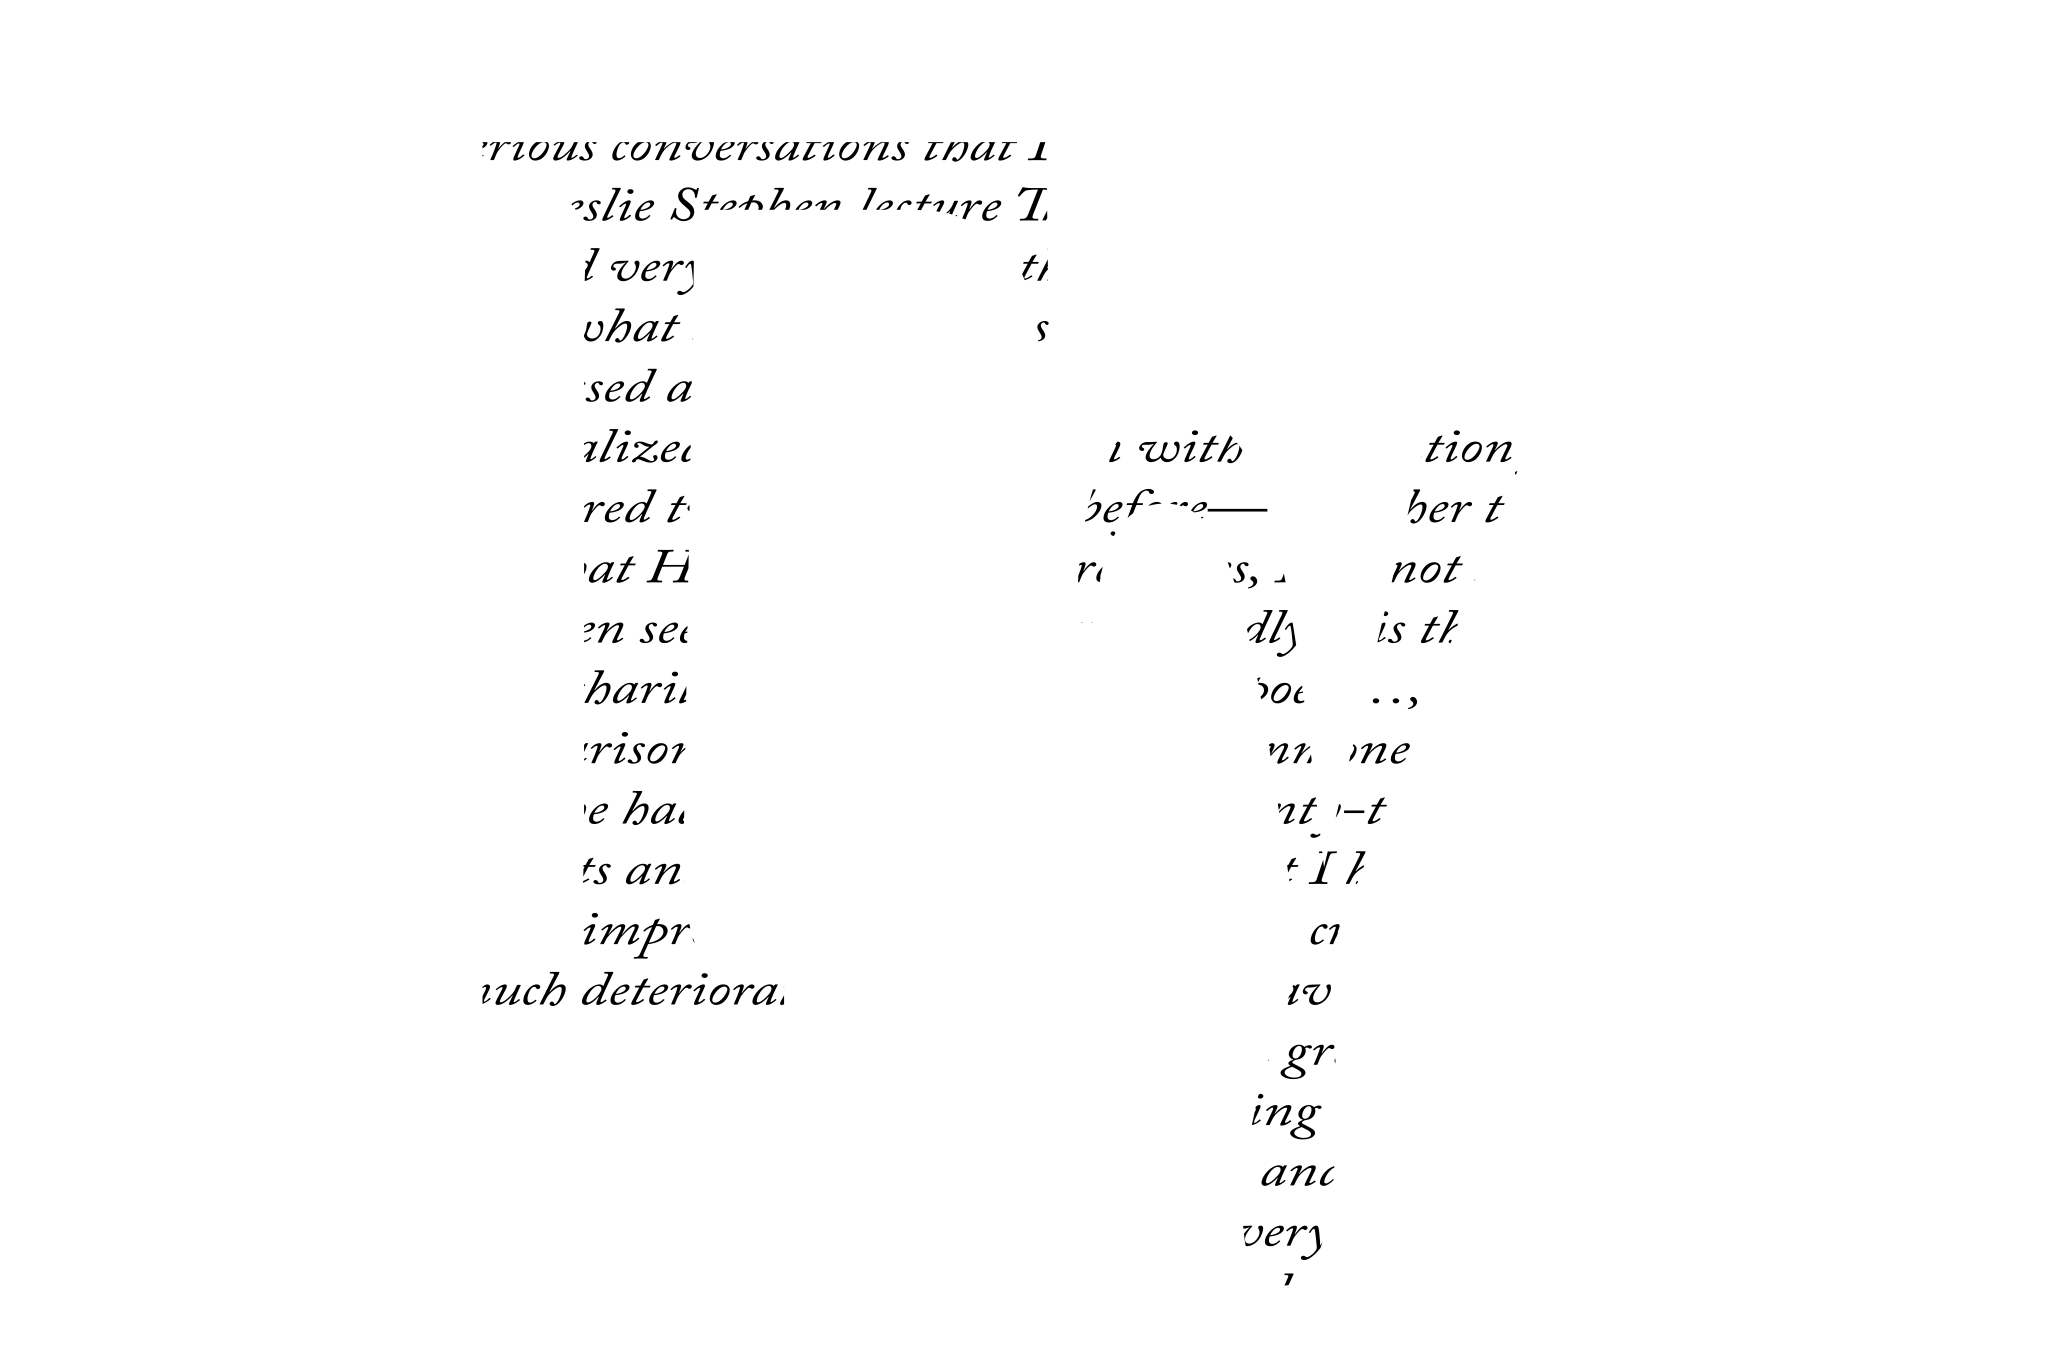
\includegraphics[scale=0.25]{immagini/gamma_illustrata.png}
	\end{figure}
	\vspace*{\fill}
\pagestyle{fancy}
	\begin{appendices}
		\chapter{Notazione multi-indice}

La notazione multi-indice è una notazione matematica che consente di semplificare enormemente la scrittura di formule matematiche. Ciò è possibile \emph{generalizzando} il concetto di indice che passa dall'essere
un semplice "numero" ad una $n-$upla ordinata di indici. Consideriamo $\alpha \in \mathbb{N}^n$, ovvero $\alpha = (\alpha_1, \ldots, \alpha_n)$ come nostro multi-indice, allora possiamo definire una serie di operazioni: la più semplice di tutti, data la natura di spazio vettoriale di cui gode $\mathbb{N}^n$, è sicuramente la somma dei multi-indici:
$$
\forall \alpha, \beta \in \mathbb{N}^n, \alpha \pm \beta = (\alpha_1 \pm \beta_1, \ldots, \alpha_n \pm \beta_n).
$$
Per quanto riguarda i nostri scopi, è utile definire la \emph{norma multi-indice}, il \emph{fattoriale multi-indice} e il \emph{coefficiente multinomiale}:
\begin{definition}[norma multi-indice]
	Sia $\alpha \in \mathbb{N}^n$ allora definiamo la norma multi-indice come
	$$
	|\alpha| = \sum_{i=1}^n \alpha_i
	$$
\end{definition}
\begin{definition}[fattoriale multi-indice]
	Sia $\alpha \in \mathbb{N}^n$, definiamo il fattoriale multi-indice di $\alpha$ come
	$$
	\alpha! = \alpha_1 ! \alpha_2 ! \ldots \alpha_n !
	$$
\end{definition}
\begin{definition}[coefficiente multinomiale]
	Sia $\alpha \in \mathbb{N}^n$ tale che $|\alpha| = k$, allora definiamo il coefficiente multinomiale come
	$$
	\binom{k}{\bm{\alpha}} = \frac{k!}{\alpha!} = \frac{k!}{\alpha_1 ! \alpha_2 ! \ldots \alpha_n !}
	$$
\end{definition}
\textbf{Notazione}: per distinguerlo dal normale coefficiente binomiale, nel caso del coefficiente multinomiale, metterò in grassetto il multi-indice.
\begin{remark}
	Potremmo pensino introdurre un ordinamento parziale (ma non è di grande interesse) dicendo che $\alpha \leq \beta \iff \alpha_i \leq \beta_i \, \, \forall i \in \{1, \ldots, n \}$. Si vede subito che, così come è stato definito, questo non può essere un ordinamento totale
\end{remark}
Vediamo come questa notazione può agevolarci la scrittura del polinomio di Taylor e la scrittura dei polinomi in $n$-variabili. Innanzitutto definiamo
\begin{definition}[potenza multi-indice]
	Sia $x \in \mathbb{R}^n$ allora
	\begin{align*}
		x^{\alpha} = x_1^{\alpha_1} x_2^{\alpha_2} \ldots x_n^{\alpha_n}
	\end{align*}
\end{definition}
Questa notazione facilita enormemente la scrittura dei polinomi in $n-$variabili, infatti
\begin{definition}[polinomio in $n-$variabili]
	$P: \mathbb{R}^n \to \mathbb{R}$ è un polinomio in $n-$variabili di grado $k \geq 0$ se
	$$
	\exists C = \{c_\alpha : |\alpha| \leq k, \alpha \in \mathbb{N}^n \} \subset \mathbb{R} 
	$$
	dove $0 \neq c_\beta \in C$ e $|\beta| = k$. Allora
	$$
	P(x) = \sum_{|\alpha| \leq k} c_\alpha x^{\alpha}
	$$
\end{definition}
Oltre a questo possiamo definire la derivata multi-indice
\begin{definition}[derivata multi-indice]
	Sia $\alpha \in \mathbb{N}^n$ allora 
	$$
	\partial^{\alpha}_x = \partial_{x_1}^{\alpha_1} \ldots \partial_{x_n}^{\alpha_n}
	$$
	dove, naturalmente, poniamo che $\partial_{x_j}^0 = 1$
\end{definition}
Riprendiamo il polinomio di Taylor: da quanto visto nella sezione \ref{sec:polinomio_taylor} abbiamo visto che possiamo scrivere il polinomio di Taylor di una funzione $f: \mathbb{R}^n \to \mathbb{R}$ come
$$
P_k(f, \xi)\sum_{i_1, \ldots, i_k=1}^k \partial_{x_{i_1}} \ldots \partial_{x_{i_k}} f(\xi) (x_{i_1} - \xi_{i_1}) \ldots (x_{i_k} - \xi_{i_k}).
$$
Osserviamo che possiamo allora usare la potenza multi-indice per scrivere i termini $(x_{i_j} - \xi_{i_j})$, considerando $\alpha \in \mathbb{N}^n$ e osservando che $\alpha_{j_1}, \ldots, \alpha_{j_m} \geq 1$ e $1 \leq j_1, \ldots, j_m \leq n$ tali che $\alpha_{j_1} + \ldots + \alpha_{j_m} = k$. In altre parole avremo solamente le derivate di ordine superiore
$$
\partial_{x_{j_1}}^{\alpha_{j_1}} \partial_{x_{j_2}}^{\alpha_{j_2}} \ldots \partial_{x_{j_m}}^{\alpha_{j_m}} f(\xi)
$$
e $\alpha_i = 0$ se $i \neq j_1, \ldots, j_m$. \\
Adesso ricordiamo che il teorema di Schwarz ci assicura che la derivata di una funzione di ordine $C^k$ rispetto agli indici $\alpha_{j_1}, \ldots, \alpha_{j_m}$ (rispetto, naturalmente, in ordine a $x_{j_1}, \ldots, x_{j_m}$) è pari a quella ottenuta con una permutazione $\sigma$ degli indici $\alpha_{j_1}, \ldots, \alpha_{j_m}$, dunque dobbiamo moltiplicare i termini della serie di Taylor per un termine che ci "tronca" i termini uguali (si ricordi la dimostrazione della proposizione \ref{prop:caratterizzazione_taylor}, dove compariva il termine $l!$). La possibilità di avere $\alpha_{j_1}$ derivate rispetto a $x_{j_1}$ sulle $k$ possibili è pari a $\binom{k}{\alpha_{j_1}}$ (non siamo interessati all'ordine, dunque usiamo per questo il coefficiente binomiale) e la stessa cosa vale per tutti gli altri termini, infatti
le possibilità di avere $\alpha_{j_2}$ derivate rispetto a $x_{j_2}$ sulle $k-\alpha_{j_1}$ rimanenti è pari a $\binom{k - \alpha_{j_1}}{\alpha_{j_2}}$ e così via. In generale, il numero di modi in cui possiamo distribuire le derivate è pari a
\begin{flalign*}
&\binom{k}{\alpha_{j_1}} \binom{k - \alpha_{j_1}}{\alpha_{j_2}} \ldots \binom{k - \alpha_{j_1} - \ldots - \alpha_{j_{m-1}}}{\alpha_{j_m}} = \\
& = \frac{k!}{\alpha_{j_1}! \cancel{(k - \alpha_{j_1})!}} \frac{\cancel{(k-\alpha_{j_1})!}}{\alpha_{j_2}!\cancel{(k - \alpha_{j_1} - \alpha_{j_2})!}} \frac{\cancel{(k - \alpha_{j_1} - \alpha_{j_2})!}}{\alpha_{j_3}! \cancel{(k - \alpha_{j_1} - \alpha_{j_2} - \alpha_{j_3})!}} \ldots \frac{\cancel{\alpha_{j_m}}}{\alpha_{j_m}! 0!} = \\
&= \frac{k!}{\alpha_{j_1}! \alpha_{j_2}! \ldots \alpha_{j_m}!} = \binom{k}{\bm{\alpha}}
\end{flalign*}
Con gli argomenti precedenti in combinazione con il teorema di Schwarz di ordine superiore, possiamo dunque dimostrare il seguente lemma
\begin{lemma}
	Sia $f \in C^k(\Omega)$ e $\xi \in \Omega$, allora abbiamo
	$$
	d^l f(\xi)(x - \xi) = \sum_{|\alpha|=l} \binom{l}{\bm{\alpha}} \partial^{\alpha} f(\xi) (x - \xi)^{\alpha}.
	$$
\end{lemma}
\begin{prop}
	Se $f \in C^k(\Omega), \Omega \subseteq \mathbb{R}^n$ aperto e $\xi \in \Omega$, allora abbiamo che
	$$
	P_k(f, \xi)(x) = \sum_{|\alpha| \leq k} \frac{1}{\alpha!} \partial^{\alpha} f(\xi) (x - \xi)^{\alpha}
	$$
\end{prop}
\begin{proof}
	Sappiamo che per $0 \leq j \leq k$ abbiamo che
	$$
	d^j f(\xi)(h) = \sum_{|\alpha| = j} \binom{j}{\bm{\alpha}} \partial^{\alpha} f(\xi) h^{\alpha}
	$$
	e ciò implica, per quanto visto nel capitolo 3, che
	\begin{align*}
	&P_k(f, \xi) = \sum_{j=0}^k \frac{1}{j!} d^j f(\xi)(x - \xi) = \sum_{j=0}^k \frac{1}{j!} \sum_{|\alpha| = j} \binom{j}{\bm{\alpha}} \partial^{\alpha}_x f(\xi) (x - \xi)^{\alpha} \stackrel{\binom{j}{\bm{\alpha}} = \frac{j!}{\bm{\alpha}!}}{=} \\
	&\stackrel{\binom{j}{\bm{\alpha}} = \frac{j!}{\bm{\alpha}!}}{=} \sum_{j=0}^k \sum_{|\alpha| = j} \frac{1}{\alpha!} \partial^{\alpha}_x f(\xi) (x - \xi)^{\alpha} = \sum_{0 \leq |\alpha| \leq k} \frac{1}{\alpha!} \partial^{\alpha}_x f(\xi) (x - \xi)^{\alpha}
	\end{align*}
\end{proof}
\begin{theorem}[formula di Taylor coi multi-indici]
	Se $f \in C^k(\Omega), \xi \in \Omega, \Omega \subseteq \mathbb{R}^n$ aperto, allora abbiamo che
	$$
	f(x) = \sum_{0 \leq |\alpha| \leq k} \frac{1}{\alpha!} \partial_x^{\alpha} f(\xi) (x - \xi)^{\alpha} + o(|x-\xi|^{\alpha})
	$$
\end{theorem}
\begin{proof}
	La dimostrazione segue dalla precedente proposizione e dalla formula di Taylor che abbiamo visto nel capitolo 3.
\end{proof}
	\end{appendices}
	\cleardoublepage
	\addcontentsline{toc}{chapter}{Bibliografia}
	\bibliographystyle{unsrt}
	\bibliography{bibliography.bib}
\end{document}